\documentclass[a4paper]{book}
\usepackage{makeidx}
\usepackage{graphicx}
\usepackage{multicol}
\usepackage{float}
\usepackage{listings}
\usepackage{color}
\usepackage{ifthen}
\usepackage[table]{xcolor}
\usepackage{textcomp}
\usepackage{alltt}
\usepackage{ifpdf}
\ifpdf
\usepackage[pdftex,
            pagebackref=true,
            colorlinks=true,
            linkcolor=blue,
            unicode
           ]{hyperref}
\else
\usepackage[ps2pdf,
            pagebackref=true,
            colorlinks=true,
            linkcolor=blue,
            unicode
           ]{hyperref}
\usepackage{pspicture}
\fi
\usepackage[utf8]{inputenc}
\usepackage{mathptmx}
\usepackage[scaled=.90]{helvet}
\usepackage{courier}
\usepackage{doxygen}
\lstset{language=C++,inputencoding=utf8,basicstyle=\footnotesize,breaklines=true,breakatwhitespace=true,tabsize=8,numbers=left }
\makeindex
\setcounter{tocdepth}{3}
\renewcommand{\footrulewidth}{0.4pt}
\begin{document}
\hypersetup{pageanchor=false}
\begin{titlepage}
\vspace*{7cm}
\begin{center}
{\Large Kinect-\/RGBD-\/GraphSLAM6D }\\
\vspace*{1cm}
{\large Generated by Doxygen 1.7.3}\\
\vspace*{0.5cm}
{\small Sun Feb 12 2012 11:52:03}\\
\end{center}
\end{titlepage}
\clearemptydoublepage
\pagenumbering{roman}
\tableofcontents
\clearemptydoublepage
\pagenumbering{arabic}
\hypersetup{pageanchor=true}
\chapter{Documentation Overview}
\label{index}\hypertarget{index}{}\hypertarget{index_intro_sec}{}\section{Introduction}\label{index_intro_sec}
This is the documentation of the Kinect-\/RGBD-\/GraphSLAM6D Final Year Project. This project integrates state-\/of-\/the-\/art algorithms to generate 3D maps using a hand-\/held Kinect sensor. The provided solution is intended to take advantage of the two main sensors that the Microsoft Kinect device contains, which are the RGB camera and the range sensor. A first approximation to the trajectory of the sensor is estimated using a pairwise alignment approach using consecutive point clouds. To avoid cummulative error this project uses a GraphSLAM approach, that mitigates the drift in the trajectory and therefore, inconsistencies in the map. \hypertarget{index_dependencies_sec}{}\section{Dependencies}\label{index_dependencies_sec}
This project integrates several open-\/source libraries to build the whole solution. The main dependencies are:
\begin{DoxyItemize}
\item OpenCV: \href{http://opencv.willowgarage.com/wiki/}{\tt http://opencv.willowgarage.com/wiki/}
\item PCL: \href{http://pointclouds.org/}{\tt http://pointclouds.org/}
\item MRPT: \href{http://www.mrpt.org/}{\tt http://www.mrpt.org/}
\item GICP: \href{http://www.stanford.edu/~avsegal/generalized_icp.html}{\tt http://www.stanford.edu/$\sim$avsegal/generalized\_\-icp.html}
\item G2O: \href{http://openslam.org/g2o}{\tt http://openslam.org/g2o}
\item Eigen: \href{http://eigen.tuxfamily.org}{\tt http://eigen.tuxfamily.org}
\item Auxiliary libraries
\begin{DoxyEnumerate}
\item FLANN
\item ANN
\item GSL
\item SuiteSparse
\item OpenNI
\item libfreenect
\item Boost
\item VTK
\item CUDA
\end{DoxyEnumerate}
\end{DoxyItemize}\hypertarget{index_install_sec}{}\section{Installation}\label{index_install_sec}
This project has been implemented and tested in Ubuntu 11.04. To compile the source code you need to install the dependencies first. After that, follow the following steps to compile the project.
\begin{DoxyItemize}
\item Compile the GICP library.
\begin{DoxyEnumerate}
\item Download the GICP library inside the KinectSLAM6D root directory. The source code of the GICP library can be found in the following link. \par
 \href{http://www.stanford.edu/~avsegal/generalized_icp.html}{\tt http://www.stanford.edu/$\sim$avsegal/generalized\_\-icp.html}
\item Compile ANN library using the following commands: \par
 \begin{DoxyVerb}
cd KinectSLAM6D/gicp/ann_1.1.1
make linux-g++
\end{DoxyVerb}

\item Compile the GICP library using the following commands: \par
 \begin{DoxyVerb}
cd KinectSLAM6D/gicp
make
\end{DoxyVerb}

\end{DoxyEnumerate}
\end{DoxyItemize}


\begin{DoxyItemize}
\item Get the G2O library (tested with revision 23).
\begin{DoxyEnumerate}
\item Download the g2o library inside the KinectSLAM6D root directory using the following commands. \begin{DoxyVerb}
cd KinectSLAM6D
svn co https://svn.openslam.org/data/svn/g2o
\end{DoxyVerb}

\end{DoxyEnumerate}
\end{DoxyItemize}


\begin{DoxyItemize}
\item Generate the Code::Blocks project.
\begin{DoxyEnumerate}
\item Open CMake.
\item Set the source directory to KinectSLAM6D and the build directory to KinectSLAM6D/build.
\item Set OpenCV\_\-DIR and MRPT\_\-DIR to the OpenCV and MRPT build directories respectively.
\item Configure.
\item Generate.
\end{DoxyEnumerate}
\end{DoxyItemize}


\begin{DoxyItemize}
\item Compile the KinectSLAM6D project.
\begin{DoxyEnumerate}
\item Open the KinectSLAM6D/build/KinectSLAM6D.cbp project.
\item Compile.
\end{DoxyEnumerate}
\end{DoxyItemize}


\begin{DoxyItemize}
\item Install CVPR tools (optional).
\begin{DoxyEnumerate}
\item Install the CVPR tools dependencies.
\item Download the CVPR tools in the KinectSLAM6D/tools directory. The set of tools can be found in the following link. \par
 \href{https://cvpr.in.tum.de/data/datasets/rgbd-dataset/tools}{\tt https://cvpr.in.tum.de/data/datasets/rgbd-\/dataset/tools} \begin{DoxyVerb}
cd KinectSLAM6D/tools
svn co https://svncvpr.in.tum.de/cvpr-ros-pkg/trunk/rgbd_benchmark/rgbd_benchmark_tools/src/rgbd_benchmark_tools
\end{DoxyVerb}

\end{DoxyEnumerate}
\end{DoxyItemize}\hypertarget{index_usage_sec}{}\section{Software usage}\label{index_usage_sec}
After compiling the project, two executables should appear in the KinectSLAM6D/build directory. The program PairwiseAlignmentSteps shows visually the steps performed in the stage of Pairwise Alignment. The program Kinect6DSLAM generates 3D maps from the provided RGB-\/D data. The RGB-\/D data can be provided using three different interfaces: two of them grabs RGB-\/D frames directly from the Kinect sensor (online). These two interfaces use the MRPT or PCL libraries to access the Kinect data. The last interface grabs RGB-\/D frames from .rawlog datasets using the MRPT library. In the following link there are some RGB-\/D datasets (.rawlog) that can be used to test the programs. To change between different configurations, set the proper \#define's in the kinect6DSLAM.cpp and PairwiseAlignmentSteps.cpp files.

\href{http://www.mrpt.org/robotic_datasets}{\tt http://www.mrpt.org/robotic\_\-datasets}

The original datasets can be found in the following link. However they are not prepared to be used in this sofware.

\href{http://cvpr.in.tum.de/data/datasets/rgbd-dataset}{\tt http://cvpr.in.tum.de/data/datasets/rgbd-\/dataset}

These RGB-\/D datasets also contain a very precise ground-\/truth that can be very useful to evaluate different configurations. In the previous link, the CVPR group also provides a set of tools to measure the error between the estimated trajectory and the real trajectory of the ground-\/truth.\hypertarget{index_PairwiseAlignmentSteps}{}\subsection{PairwiseAlignmentSteps}\label{index_PairwiseAlignmentSteps}
This program performs Pairwise Alignment between two RGB-\/D frames selected by the user. This program aims to show visually the different steps that occur during the Pairwise Alignment process. This program requires the user to select two RGB-\/D frames of the sequence data. Press \char`\"{}enter\char`\"{} in the OpenCV window to select an RGB-\/D frame. The program stores the results of the alignment in the KinectSLAM6D/results directory.

\begin{DoxyVerb}
cd KinectSLAM6D/build
./PairwiseAlignmentSteps [* <rgbd_dataset>.rawlog]
\end{DoxyVerb}
 \mbox{[}$\ast$\mbox{]} Optional parameter to provide a RGB-\/D dataset.

   \hypertarget{index_Kinect6DSLAM}{}\subsection{Kinect6DSLAM}\label{index_Kinect6DSLAM}
This program generates a 3D map from the provided secuence of RGB-\/D frames. This program requires the user to press enter to stop grabbing RGB-\/D frames. The program stores the results of the alignment in the KinectSLAM6D/results directory. The program generates .pcd files that contain a global point cloud representing the 3D map. These files are generated in the KinectSLAM6D/results/pcd\_\-files directory. The estimated trajectory files and GraphSLAM graphs are generated in the KinectSLAM6D/results/graphs directory.

\begin{DoxyVerb}
cd KinectSLAM6D/build
./KinectSLAM6D [* <rgbd_dataset>.rawlog] [** <grount_truth>.txt]
\end{DoxyVerb}
 \mbox{[}$\ast$\mbox{]} Optional parameter to provide a RGB-\/D dataset. \par
 \mbox{[}$\ast$$\ast$\mbox{]} Optional parameter to provide the ground-\/truth of the RGB-\/D dataset. (requires the CVPR tools and depencencies installed)

   \begin{DoxyAuthor}{Author}
Miguel Algaba Borrego \par
 \href{http://thecomputervision.blogspot.com/}{\tt http://thecomputervision.blogspot.com/} 
\end{DoxyAuthor}

\chapter{Data Structure Index}
\section{Class Hierarchy}
This inheritance list is sorted roughly, but not completely, alphabetically:\begin{DoxyCompactList}
\item \contentsline{section}{FrameRGBD}{\pageref{class_frame_r_g_b_d}}{}
\item \contentsline{section}{GraphOptimizer}{\pageref{class_graph_optimizer}}{}
\begin{DoxyCompactList}
\item \contentsline{section}{GraphOptimizer\_\-G2O}{\pageref{class_graph_optimizer___g2_o}}{}
\item \contentsline{section}{GraphOptimizer\_\-MRPT}{\pageref{class_graph_optimizer___m_r_p_t}}{}
\end{DoxyCompactList}
\item \contentsline{section}{ICPPoseRefiner}{\pageref{class_i_c_p_pose_refiner}}{}
\begin{DoxyCompactList}
\item \contentsline{section}{ICPPoseRefiner\_\-PCL}{\pageref{class_i_c_p_pose_refiner___p_c_l}}{}
\item \contentsline{section}{ICPPoseRefiner\_\-StanfordGICP}{\pageref{class_i_c_p_pose_refiner___stanford_g_i_c_p}}{}
\end{DoxyCompactList}
\item \contentsline{section}{KeyframeLoopDetector}{\pageref{class_keyframe_loop_detector}}{}
\item \contentsline{section}{KinectGrabber}{\pageref{class_kinect_grabber}}{}
\begin{DoxyCompactList}
\item \contentsline{section}{KinectGrabber\_\-MRPT}{\pageref{class_kinect_grabber___m_r_p_t}}{}
\item \contentsline{section}{KinectGrabber\_\-OpenNI}{\pageref{class_kinect_grabber___open_n_i}}{}
\item \contentsline{section}{KinectGrabber\_\-Rawlog}{\pageref{class_kinect_grabber___rawlog}}{}
\end{DoxyCompactList}
\item \contentsline{section}{PointCloudDownsampler}{\pageref{class_point_cloud_downsampler}}{}
\item \contentsline{section}{PointCloudViewer}{\pageref{class_point_cloud_viewer}}{}
\begin{DoxyCompactList}
\item \contentsline{section}{PointCloudViewer\_\-MRPT}{\pageref{class_point_cloud_viewer___m_r_p_t}}{}
\end{DoxyCompactList}
\item \contentsline{section}{KinectGrabber\_\-MRPT::TThreadParam}{\pageref{struct_kinect_grabber___m_r_p_t_1_1_t_thread_param}}{}
\item \contentsline{section}{KinectGrabber\_\-Rawlog::TThreadParam}{\pageref{struct_kinect_grabber___rawlog_1_1_t_thread_param}}{}
\item \contentsline{section}{Visual3DRigidTransformationEstimator}{\pageref{class_visual3_d_rigid_transformation_estimator}}{}
\begin{DoxyCompactList}
\item \contentsline{section}{Visual3DRigidTransformationEstimator\_\-RANSAC}{\pageref{class_visual3_d_rigid_transformation_estimator___r_a_n_s_a_c}}{}
\item \contentsline{section}{Visual3DRigidTransformationEstimator\_\-SVD}{\pageref{class_visual3_d_rigid_transformation_estimator___s_v_d}}{}
\end{DoxyCompactList}
\item \contentsline{section}{VisualFeatureDescriptorExtractor}{\pageref{class_visual_feature_descriptor_extractor}}{}
\begin{DoxyCompactList}
\item \contentsline{section}{VisualFeatureDescriptorExtractor\_\-Generic}{\pageref{class_visual_feature_descriptor_extractor___generic}}{}
\item \contentsline{section}{VisualFeatureDescriptorExtractor\_\-ORB}{\pageref{class_visual_feature_descriptor_extractor___o_r_b}}{}
\item \contentsline{section}{VisualFeatureDescriptorExtractor\_\-SURF\_\-GPU}{\pageref{class_visual_feature_descriptor_extractor___s_u_r_f___g_p_u}}{}
\end{DoxyCompactList}
\item \contentsline{section}{VisualFeatureMatcher}{\pageref{class_visual_feature_matcher}}{}
\begin{DoxyCompactList}
\item \contentsline{section}{VisualFeatureMatcher\_\-Generic}{\pageref{class_visual_feature_matcher___generic}}{}
\end{DoxyCompactList}
\end{DoxyCompactList}

\chapter{Data Structure Index}
\section{Data Structures}
Here are the data structures with brief descriptions:\begin{DoxyCompactList}
\item\contentsline{section}{\hyperlink{class_frame_r_g_b_d}{FrameRGBD} }{\pageref{class_frame_r_g_b_d}}{}
\item\contentsline{section}{\hyperlink{class_graph_optimizer}{GraphOptimizer} }{\pageref{class_graph_optimizer}}{}
\item\contentsline{section}{\hyperlink{class_graph_optimizer___g2_o}{GraphOptimizer\_\-G2O} }{\pageref{class_graph_optimizer___g2_o}}{}
\item\contentsline{section}{\hyperlink{class_graph_optimizer___m_r_p_t}{GraphOptimizer\_\-MRPT} }{\pageref{class_graph_optimizer___m_r_p_t}}{}
\item\contentsline{section}{\hyperlink{class_i_c_p_pose_refiner}{ICPPoseRefiner} }{\pageref{class_i_c_p_pose_refiner}}{}
\item\contentsline{section}{\hyperlink{class_i_c_p_pose_refiner___p_c_l}{ICPPoseRefiner\_\-PCL} }{\pageref{class_i_c_p_pose_refiner___p_c_l}}{}
\item\contentsline{section}{\hyperlink{class_i_c_p_pose_refiner___stanford_g_i_c_p}{ICPPoseRefiner\_\-StanfordGICP} }{\pageref{class_i_c_p_pose_refiner___stanford_g_i_c_p}}{}
\item\contentsline{section}{\hyperlink{class_keyframe_loop_detector}{KeyframeLoopDetector} }{\pageref{class_keyframe_loop_detector}}{}
\item\contentsline{section}{\hyperlink{class_kinect_grabber}{KinectGrabber} }{\pageref{class_kinect_grabber}}{}
\item\contentsline{section}{\hyperlink{class_kinect_grabber___m_r_p_t}{KinectGrabber\_\-MRPT} }{\pageref{class_kinect_grabber___m_r_p_t}}{}
\item\contentsline{section}{\hyperlink{class_kinect_grabber___open_n_i}{KinectGrabber\_\-OpenNI} }{\pageref{class_kinect_grabber___open_n_i}}{}
\item\contentsline{section}{\hyperlink{class_kinect_grabber___rawlog}{KinectGrabber\_\-Rawlog} }{\pageref{class_kinect_grabber___rawlog}}{}
\item\contentsline{section}{\hyperlink{class_point_cloud_downsampler}{PointCloudDownsampler} }{\pageref{class_point_cloud_downsampler}}{}
\item\contentsline{section}{\hyperlink{class_point_cloud_viewer}{PointCloudViewer} }{\pageref{class_point_cloud_viewer}}{}
\item\contentsline{section}{\hyperlink{class_point_cloud_viewer___m_r_p_t}{PointCloudViewer\_\-MRPT} }{\pageref{class_point_cloud_viewer___m_r_p_t}}{}
\item\contentsline{section}{\hyperlink{struct_kinect_grabber___m_r_p_t_1_1_t_thread_param}{KinectGrabber\_\-MRPT::TThreadParam} }{\pageref{struct_kinect_grabber___m_r_p_t_1_1_t_thread_param}}{}
\item\contentsline{section}{\hyperlink{struct_kinect_grabber___rawlog_1_1_t_thread_param}{KinectGrabber\_\-Rawlog::TThreadParam} }{\pageref{struct_kinect_grabber___rawlog_1_1_t_thread_param}}{}
\item\contentsline{section}{\hyperlink{class_visual3_d_rigid_transformation_estimator}{Visual3DRigidTransformationEstimator} }{\pageref{class_visual3_d_rigid_transformation_estimator}}{}
\item\contentsline{section}{\hyperlink{class_visual3_d_rigid_transformation_estimator___r_a_n_s_a_c}{Visual3DRigidTransformationEstimator\_\-RANSAC} }{\pageref{class_visual3_d_rigid_transformation_estimator___r_a_n_s_a_c}}{}
\item\contentsline{section}{\hyperlink{class_visual3_d_rigid_transformation_estimator___s_v_d}{Visual3DRigidTransformationEstimator\_\-SVD} }{\pageref{class_visual3_d_rigid_transformation_estimator___s_v_d}}{}
\item\contentsline{section}{\hyperlink{class_visual_feature_descriptor_extractor}{VisualFeatureDescriptorExtractor} }{\pageref{class_visual_feature_descriptor_extractor}}{}
\item\contentsline{section}{\hyperlink{class_visual_feature_descriptor_extractor___generic}{VisualFeatureDescriptorExtractor\_\-Generic} }{\pageref{class_visual_feature_descriptor_extractor___generic}}{}
\item\contentsline{section}{\hyperlink{class_visual_feature_descriptor_extractor___o_r_b}{VisualFeatureDescriptorExtractor\_\-ORB} }{\pageref{class_visual_feature_descriptor_extractor___o_r_b}}{}
\item\contentsline{section}{\hyperlink{class_visual_feature_descriptor_extractor___s_u_r_f___g_p_u}{VisualFeatureDescriptorExtractor\_\-SURF\_\-GPU} }{\pageref{class_visual_feature_descriptor_extractor___s_u_r_f___g_p_u}}{}
\item\contentsline{section}{\hyperlink{class_visual_feature_matcher}{VisualFeatureMatcher} }{\pageref{class_visual_feature_matcher}}{}
\item\contentsline{section}{\hyperlink{class_visual_feature_matcher___generic}{VisualFeatureMatcher\_\-Generic} }{\pageref{class_visual_feature_matcher___generic}}{}
\end{DoxyCompactList}

\chapter{Data Structure Documentation}
\hypertarget{class_frame_r_g_b_d}{
\section{FrameRGBD Class Reference}
\label{class_frame_r_g_b_d}\index{FrameRGBD@{FrameRGBD}}
}


{\ttfamily \#include $<$FrameRGBD.h$>$}

\subsection*{Public Member Functions}
\begin{DoxyCompactItemize}
\item 
void \hyperlink{class_frame_r_g_b_d_ac3f882e82c847c18e817c988f1f47e6f}{computeGICPNormalMatrices} (const double=1e-\/3)
\end{DoxyCompactItemize}
\subsection*{Data Fields}
\begin{DoxyCompactItemize}
\item 
pcl::PointCloud$<$ pcl::PointXYZRGB $>$::Ptr \hyperlink{class_frame_r_g_b_d_a03899f04e6597201e13fb2e046fd0983}{pointCloudPtr}
\item 
pcl::PointCloud$<$ pcl::PointXYZRGB $>$::Ptr \hyperlink{class_frame_r_g_b_d_a7c5a9dcf60d9ee1ac6d4d707257e965f}{downsampledPointCloudPtr}
\item 
cv::Mat \hyperlink{class_frame_r_g_b_d_a198aed26e98378616a1aee67f1e32182}{intensityImage}
\item 
dgc::gicp::GICPPointSet \hyperlink{class_frame_r_g_b_d_aeadd4cb8c9658d6b995ce72d9bef200d}{gicpPointSet}
\item 
\hypertarget{class_frame_r_g_b_d_a76abacf5326b11709d9f90a9dcd09817}{
uint64\_\-t {\bfseries timeStamp}}
\label{class_frame_r_g_b_d_a76abacf5326b11709d9f90a9dcd09817}

\end{DoxyCompactItemize}


\subsection{Detailed Description}
The class \hyperlink{class_frame_r_g_b_d}{FrameRGBD} encapsulates the RGB and 3D data of a certain frame. It contains the intensity image provided by the RGB camera, the 3D coloured point cloud reconstructed from the depth and RGB images. It also contains a downsampled version of the 3D point cloud. 

\subsection{Member Function Documentation}
\hypertarget{class_frame_r_g_b_d_ac3f882e82c847c18e817c988f1f47e6f}{
\index{FrameRGBD@{FrameRGBD}!computeGICPNormalMatrices@{computeGICPNormalMatrices}}
\index{computeGICPNormalMatrices@{computeGICPNormalMatrices}!FrameRGBD@{FrameRGBD}}
\subsubsection[{computeGICPNormalMatrices}]{\setlength{\rightskip}{0pt plus 5cm}void FrameRGBD::computeGICPNormalMatrices (
\begin{DoxyParamCaption}
\item[{const double}]{ = {\ttfamily 1e-\/3}}
\end{DoxyParamCaption}
)}}
\label{class_frame_r_g_b_d_ac3f882e82c847c18e817c988f1f47e6f}
Compute the point cloud normals and covariance matrices for GICP 

\subsection{Field Documentation}
\hypertarget{class_frame_r_g_b_d_a7c5a9dcf60d9ee1ac6d4d707257e965f}{
\index{FrameRGBD@{FrameRGBD}!downsampledPointCloudPtr@{downsampledPointCloudPtr}}
\index{downsampledPointCloudPtr@{downsampledPointCloudPtr}!FrameRGBD@{FrameRGBD}}
\subsubsection[{downsampledPointCloudPtr}]{\setlength{\rightskip}{0pt plus 5cm}pcl::PointCloud$<$pcl::PointXYZRGB$>$::Ptr {\bf FrameRGBD::downsampledPointCloudPtr}}}
\label{class_frame_r_g_b_d_a7c5a9dcf60d9ee1ac6d4d707257e965f}
Pointer to the downsampled version of the point cloud \hypertarget{class_frame_r_g_b_d_aeadd4cb8c9658d6b995ce72d9bef200d}{
\index{FrameRGBD@{FrameRGBD}!gicpPointSet@{gicpPointSet}}
\index{gicpPointSet@{gicpPointSet}!FrameRGBD@{FrameRGBD}}
\subsubsection[{gicpPointSet}]{\setlength{\rightskip}{0pt plus 5cm}dgc::gicp::GICPPointSet {\bf FrameRGBD::gicpPointSet}}}
\label{class_frame_r_g_b_d_aeadd4cb8c9658d6b995ce72d9bef200d}
Downsampled point cloud with normals for the GICP algorithm \hypertarget{class_frame_r_g_b_d_a198aed26e98378616a1aee67f1e32182}{
\index{FrameRGBD@{FrameRGBD}!intensityImage@{intensityImage}}
\index{intensityImage@{intensityImage}!FrameRGBD@{FrameRGBD}}
\subsubsection[{intensityImage}]{\setlength{\rightskip}{0pt plus 5cm}cv::Mat {\bf FrameRGBD::intensityImage}}}
\label{class_frame_r_g_b_d_a198aed26e98378616a1aee67f1e32182}
Grayscale intensity image \hypertarget{class_frame_r_g_b_d_a03899f04e6597201e13fb2e046fd0983}{
\index{FrameRGBD@{FrameRGBD}!pointCloudPtr@{pointCloudPtr}}
\index{pointCloudPtr@{pointCloudPtr}!FrameRGBD@{FrameRGBD}}
\subsubsection[{pointCloudPtr}]{\setlength{\rightskip}{0pt plus 5cm}pcl::PointCloud$<$pcl::PointXYZRGB$>$::Ptr {\bf FrameRGBD::pointCloudPtr}}}
\label{class_frame_r_g_b_d_a03899f04e6597201e13fb2e046fd0983}
Pointer to the coloured 3D point cloud 

The documentation for this class was generated from the following file:\begin{DoxyCompactItemize}
\item 
FrameRGBD.h\end{DoxyCompactItemize}

\hypertarget{class_graph_optimizer}{
\section{GraphOptimizer Class Reference}
\label{class_graph_optimizer}\index{GraphOptimizer@{GraphOptimizer}}
}


{\ttfamily \#include $<$GraphOptimizer.h$>$}

Inheritance diagram for GraphOptimizer:\begin{figure}[H]
\begin{center}
\leavevmode
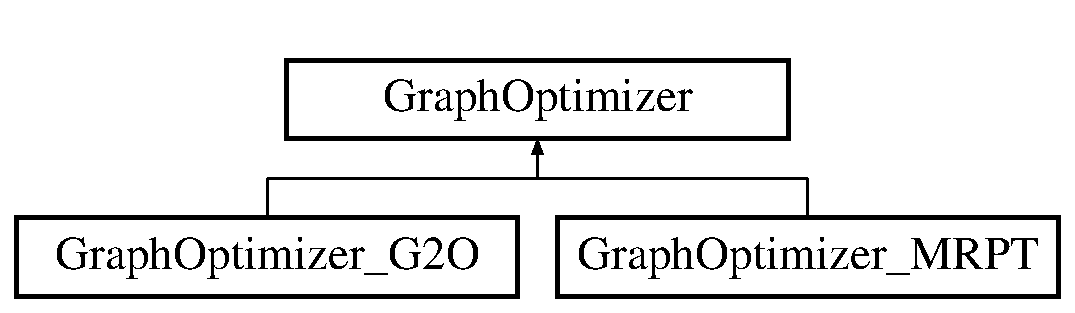
\includegraphics[height=2.000000cm]{class_graph_optimizer}
\end{center}
\end{figure}
\subsection*{Public Member Functions}
\begin{DoxyCompactItemize}
\item 
virtual int \hyperlink{class_graph_optimizer_a2acd85307e0c0a006a2360f9d7e29bce}{addVertex} (Eigen::Matrix4f \&pose)=0
\item 
virtual void \hyperlink{class_graph_optimizer_a7bf9e4c2d3376bf8af5b15c86398950e}{addEdge} (const int fromIdx, const int toIdx, Eigen::Matrix4f \&relPose, Eigen::Matrix$<$ double, 6, 6 $>$ \&infMatrix)=0
\item 
virtual void \hyperlink{class_graph_optimizer_ad1e8ac7c0aa9c90f3035c1d29036eedb}{optimizeGraph} ()=0
\item 
virtual void \hyperlink{class_graph_optimizer_a914f6c37de8dc6437122b3f563cce9a5}{getPoses} (std::vector$<$ Eigen::Matrix4f, Eigen::aligned\_\-allocator$<$ Eigen::Matrix4f $>$ $>$ \&)=0
\item 
virtual void \hyperlink{class_graph_optimizer_a303a1e4e96fa44433ef48aa4051fab32}{saveGraph} (std::string fileName)=0
\end{DoxyCompactItemize}


\subsection{Detailed Description}
Abstract class that defines the mandatory methods that a 6D GraphSLAM optimizer must implement. 

\subsection{Member Function Documentation}
\hypertarget{class_graph_optimizer_a7bf9e4c2d3376bf8af5b15c86398950e}{
\index{GraphOptimizer@{GraphOptimizer}!addEdge@{addEdge}}
\index{addEdge@{addEdge}!GraphOptimizer@{GraphOptimizer}}
\subsubsection[{addEdge}]{\setlength{\rightskip}{0pt plus 5cm}virtual void GraphOptimizer::addEdge (
\begin{DoxyParamCaption}
\item[{const int}]{fromIdx, }
\item[{const int}]{toIdx, }
\item[{Eigen::Matrix4f \&}]{relPose, }
\item[{Eigen::Matrix$<$ double, 6, 6 $>$ \&}]{infMatrix}
\end{DoxyParamCaption}
)\hspace{0.3cm}{\ttfamily  \mbox{[}pure virtual\mbox{]}}}}
\label{class_graph_optimizer_a7bf9e4c2d3376bf8af5b15c86398950e}
Adds an edge that defines a spatial constraint between the vertices \char`\"{}fromIdx\char`\"{} and \char`\"{}toIdx\char`\"{} with information matrix that determines the weight of the added edge. 

Implemented in \hyperlink{class_graph_optimizer___g2_o_a53c3edc42e43fef29e4a945141654391}{GraphOptimizer\_\-G2O}, and \hyperlink{class_graph_optimizer___m_r_p_t_a593e4c3752d6e3b6340145e5fd03ad92}{GraphOptimizer\_\-MRPT}.

\hypertarget{class_graph_optimizer_a2acd85307e0c0a006a2360f9d7e29bce}{
\index{GraphOptimizer@{GraphOptimizer}!addVertex@{addVertex}}
\index{addVertex@{addVertex}!GraphOptimizer@{GraphOptimizer}}
\subsubsection[{addVertex}]{\setlength{\rightskip}{0pt plus 5cm}virtual int GraphOptimizer::addVertex (
\begin{DoxyParamCaption}
\item[{Eigen::Matrix4f \&}]{pose}
\end{DoxyParamCaption}
)\hspace{0.3cm}{\ttfamily  \mbox{[}pure virtual\mbox{]}}}}
\label{class_graph_optimizer_a2acd85307e0c0a006a2360f9d7e29bce}
Adds a new vertex to the graph. The provided 4x4 matrix will be considered as the pose of the new added vertex. It returns the index of the added vertex. 

Implemented in \hyperlink{class_graph_optimizer___g2_o_ad1c9376f78767de3063170221e43859a}{GraphOptimizer\_\-G2O}, and \hyperlink{class_graph_optimizer___m_r_p_t_a2c5a89fce928859445d3ec2627a0ed3e}{GraphOptimizer\_\-MRPT}.

\hypertarget{class_graph_optimizer_a914f6c37de8dc6437122b3f563cce9a5}{
\index{GraphOptimizer@{GraphOptimizer}!getPoses@{getPoses}}
\index{getPoses@{getPoses}!GraphOptimizer@{GraphOptimizer}}
\subsubsection[{getPoses}]{\setlength{\rightskip}{0pt plus 5cm}virtual void GraphOptimizer::getPoses (
\begin{DoxyParamCaption}
\item[{std::vector$<$ Eigen::Matrix4f, Eigen::aligned\_\-allocator$<$ Eigen::Matrix4f $>$ $>$ \&}]{}
\end{DoxyParamCaption}
)\hspace{0.3cm}{\ttfamily  \mbox{[}pure virtual\mbox{]}}}}
\label{class_graph_optimizer_a914f6c37de8dc6437122b3f563cce9a5}
Returns a vector with all the optimized poses of the graph. 

Implemented in \hyperlink{class_graph_optimizer___g2_o_ad30f6cd46b424482a7b26e41fb442f50}{GraphOptimizer\_\-G2O}, and \hyperlink{class_graph_optimizer___m_r_p_t_a40f1548815f2830a950bb682782793b7}{GraphOptimizer\_\-MRPT}.

\hypertarget{class_graph_optimizer_ad1e8ac7c0aa9c90f3035c1d29036eedb}{
\index{GraphOptimizer@{GraphOptimizer}!optimizeGraph@{optimizeGraph}}
\index{optimizeGraph@{optimizeGraph}!GraphOptimizer@{GraphOptimizer}}
\subsubsection[{optimizeGraph}]{\setlength{\rightskip}{0pt plus 5cm}virtual void GraphOptimizer::optimizeGraph (
\begin{DoxyParamCaption}
{}
\end{DoxyParamCaption}
)\hspace{0.3cm}{\ttfamily  \mbox{[}pure virtual\mbox{]}}}}
\label{class_graph_optimizer_ad1e8ac7c0aa9c90f3035c1d29036eedb}
Calls the graph optimization process to determine the pose configuration that best satisfies the constraints defined by the edges. 

Implemented in \hyperlink{class_graph_optimizer___g2_o_a78dac310c50fdd61bcbcc64855fe6565}{GraphOptimizer\_\-G2O}, and \hyperlink{class_graph_optimizer___m_r_p_t_aa60e33c3028018515f01aaae20ec9bd5}{GraphOptimizer\_\-MRPT}.

\hypertarget{class_graph_optimizer_a303a1e4e96fa44433ef48aa4051fab32}{
\index{GraphOptimizer@{GraphOptimizer}!saveGraph@{saveGraph}}
\index{saveGraph@{saveGraph}!GraphOptimizer@{GraphOptimizer}}
\subsubsection[{saveGraph}]{\setlength{\rightskip}{0pt plus 5cm}virtual void GraphOptimizer::saveGraph (
\begin{DoxyParamCaption}
\item[{std::string}]{fileName}
\end{DoxyParamCaption}
)\hspace{0.3cm}{\ttfamily  \mbox{[}pure virtual\mbox{]}}}}
\label{class_graph_optimizer_a303a1e4e96fa44433ef48aa4051fab32}
Saves the graph to file. 

Implemented in \hyperlink{class_graph_optimizer___g2_o_ae0aff0bbd454803fb4a32fc5bdae1a2a}{GraphOptimizer\_\-G2O}, and \hyperlink{class_graph_optimizer___m_r_p_t_a5456297ea1d91e7cafc55e3a46ee7ad6}{GraphOptimizer\_\-MRPT}.



The documentation for this class was generated from the following file:\begin{DoxyCompactItemize}
\item 
GraphOptimizer.h\end{DoxyCompactItemize}

\hypertarget{class_graph_optimizer___g2_o}{
\section{GraphOptimizer\_\-G2O Class Reference}
\label{class_graph_optimizer___g2_o}\index{GraphOptimizer\_\-G2O@{GraphOptimizer\_\-G2O}}
}


{\ttfamily \#include $<$GraphOptimizer\_\-G2O.h$>$}

Inheritance diagram for GraphOptimizer\_\-G2O:\begin{figure}[H]
\begin{center}
\leavevmode
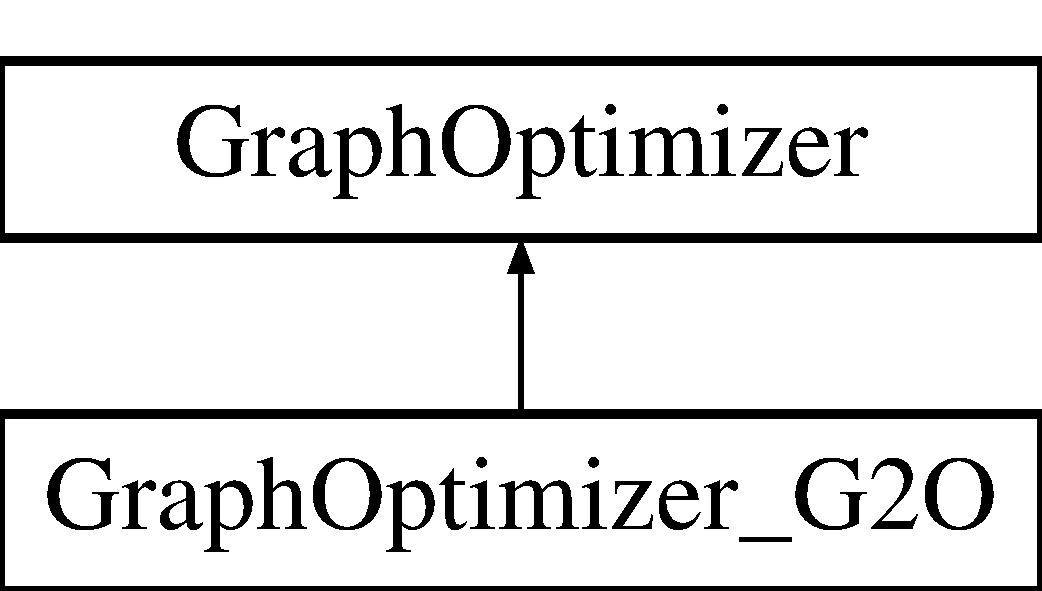
\includegraphics[height=2.000000cm]{class_graph_optimizer___g2_o}
\end{center}
\end{figure}
\subsection*{Public Member Functions}
\begin{DoxyCompactItemize}
\item 
int \hyperlink{class_graph_optimizer___g2_o_ad1c9376f78767de3063170221e43859a}{addVertex} (Eigen::Matrix4f \&pose)
\item 
void \hyperlink{class_graph_optimizer___g2_o_a53c3edc42e43fef29e4a945141654391}{addEdge} (const int fromIdx, const int toIdx, Eigen::Matrix4f \&relPose, Eigen::Matrix$<$ double, 6, 6 $>$ \&infMatrix)
\item 
void \hyperlink{class_graph_optimizer___g2_o_a78dac310c50fdd61bcbcc64855fe6565}{optimizeGraph} ()
\item 
void \hyperlink{class_graph_optimizer___g2_o_ad30f6cd46b424482a7b26e41fb442f50}{getPoses} (std::vector$<$ Eigen::Matrix4f, Eigen::aligned\_\-allocator$<$ Eigen::Matrix4f $>$ $>$ \&)
\item 
void \hyperlink{class_graph_optimizer___g2_o_ae0aff0bbd454803fb4a32fc5bdae1a2a}{saveGraph} (std::string fileName)
\end{DoxyCompactItemize}
\subsection*{Private Attributes}
\begin{DoxyCompactItemize}
\item 
\hypertarget{class_graph_optimizer___g2_o_a0663a4b590a88e4191699283ec285a66}{
int {\bfseries vertexIdx}}
\label{class_graph_optimizer___g2_o_a0663a4b590a88e4191699283ec285a66}

\item 
\hypertarget{class_graph_optimizer___g2_o_a0ad18bf592cfd85ffb981773895672bb}{
g2o::SparseOptimizer {\bfseries optimizer}}
\label{class_graph_optimizer___g2_o_a0ad18bf592cfd85ffb981773895672bb}

\item 
\hypertarget{class_graph_optimizer___g2_o_a2e15c63ca4c846615b225c0de43cb02a}{
g2o::BlockSolverX::LinearSolverType $\ast$ {\bfseries linearSolver}}
\label{class_graph_optimizer___g2_o_a2e15c63ca4c846615b225c0de43cb02a}

\item 
\hypertarget{class_graph_optimizer___g2_o_a449d9cb7982ca7728b9e6703e8e99aac}{
g2o::BlockSolverX $\ast$ {\bfseries solver\_\-ptr}}
\label{class_graph_optimizer___g2_o_a449d9cb7982ca7728b9e6703e8e99aac}

\end{DoxyCompactItemize}


\subsection{Detailed Description}
This class encapsulates the functionality of the G2O library to perform 6D graph optimization. 

\subsection{Member Function Documentation}
\hypertarget{class_graph_optimizer___g2_o_a53c3edc42e43fef29e4a945141654391}{
\index{GraphOptimizer\_\-G2O@{GraphOptimizer\_\-G2O}!addEdge@{addEdge}}
\index{addEdge@{addEdge}!GraphOptimizer_G2O@{GraphOptimizer\_\-G2O}}
\subsubsection[{addEdge}]{\setlength{\rightskip}{0pt plus 5cm}void GraphOptimizer\_\-G2O::addEdge (
\begin{DoxyParamCaption}
\item[{const int}]{fromIdx, }
\item[{const int}]{toIdx, }
\item[{Eigen::Matrix4f \&}]{relPose, }
\item[{Eigen::Matrix$<$ double, 6, 6 $>$ \&}]{infMatrix}
\end{DoxyParamCaption}
)\hspace{0.3cm}{\ttfamily  \mbox{[}virtual\mbox{]}}}}
\label{class_graph_optimizer___g2_o_a53c3edc42e43fef29e4a945141654391}
Adds an edge that defines a spatial constraint between the vertices \char`\"{}fromIdx\char`\"{} and \char`\"{}toIdx\char`\"{} with information matrix that determines the weight of the added edge. 

Implements \hyperlink{class_graph_optimizer_a7bf9e4c2d3376bf8af5b15c86398950e}{GraphOptimizer}.

\hypertarget{class_graph_optimizer___g2_o_ad1c9376f78767de3063170221e43859a}{
\index{GraphOptimizer\_\-G2O@{GraphOptimizer\_\-G2O}!addVertex@{addVertex}}
\index{addVertex@{addVertex}!GraphOptimizer_G2O@{GraphOptimizer\_\-G2O}}
\subsubsection[{addVertex}]{\setlength{\rightskip}{0pt plus 5cm}int GraphOptimizer\_\-G2O::addVertex (
\begin{DoxyParamCaption}
\item[{Eigen::Matrix4f \&}]{pose}
\end{DoxyParamCaption}
)\hspace{0.3cm}{\ttfamily  \mbox{[}virtual\mbox{]}}}}
\label{class_graph_optimizer___g2_o_ad1c9376f78767de3063170221e43859a}
Adds a new vertex to the graph. The provided 4x4 matrix will be considered as the pose of the new added vertex. It returns the index of the added vertex. 

Implements \hyperlink{class_graph_optimizer_a2acd85307e0c0a006a2360f9d7e29bce}{GraphOptimizer}.

\hypertarget{class_graph_optimizer___g2_o_ad30f6cd46b424482a7b26e41fb442f50}{
\index{GraphOptimizer\_\-G2O@{GraphOptimizer\_\-G2O}!getPoses@{getPoses}}
\index{getPoses@{getPoses}!GraphOptimizer_G2O@{GraphOptimizer\_\-G2O}}
\subsubsection[{getPoses}]{\setlength{\rightskip}{0pt plus 5cm}void GraphOptimizer\_\-G2O::getPoses (
\begin{DoxyParamCaption}
\item[{std::vector$<$ Eigen::Matrix4f, Eigen::aligned\_\-allocator$<$ Eigen::Matrix4f $>$ $>$ \&}]{}
\end{DoxyParamCaption}
)\hspace{0.3cm}{\ttfamily  \mbox{[}virtual\mbox{]}}}}
\label{class_graph_optimizer___g2_o_ad30f6cd46b424482a7b26e41fb442f50}
Returns a vector with all the optimized poses of the graph. 

Implements \hyperlink{class_graph_optimizer_a914f6c37de8dc6437122b3f563cce9a5}{GraphOptimizer}.

\hypertarget{class_graph_optimizer___g2_o_a78dac310c50fdd61bcbcc64855fe6565}{
\index{GraphOptimizer\_\-G2O@{GraphOptimizer\_\-G2O}!optimizeGraph@{optimizeGraph}}
\index{optimizeGraph@{optimizeGraph}!GraphOptimizer_G2O@{GraphOptimizer\_\-G2O}}
\subsubsection[{optimizeGraph}]{\setlength{\rightskip}{0pt plus 5cm}void GraphOptimizer\_\-G2O::optimizeGraph (
\begin{DoxyParamCaption}
{}
\end{DoxyParamCaption}
)\hspace{0.3cm}{\ttfamily  \mbox{[}virtual\mbox{]}}}}
\label{class_graph_optimizer___g2_o_a78dac310c50fdd61bcbcc64855fe6565}
Calls the graph optimization process to determine the pose configuration that best satisfies the constraints defined by the edges. 

Implements \hyperlink{class_graph_optimizer_ad1e8ac7c0aa9c90f3035c1d29036eedb}{GraphOptimizer}.

\hypertarget{class_graph_optimizer___g2_o_ae0aff0bbd454803fb4a32fc5bdae1a2a}{
\index{GraphOptimizer\_\-G2O@{GraphOptimizer\_\-G2O}!saveGraph@{saveGraph}}
\index{saveGraph@{saveGraph}!GraphOptimizer_G2O@{GraphOptimizer\_\-G2O}}
\subsubsection[{saveGraph}]{\setlength{\rightskip}{0pt plus 5cm}void GraphOptimizer\_\-G2O::saveGraph (
\begin{DoxyParamCaption}
\item[{std::string}]{fileName}
\end{DoxyParamCaption}
)\hspace{0.3cm}{\ttfamily  \mbox{[}virtual\mbox{]}}}}
\label{class_graph_optimizer___g2_o_ae0aff0bbd454803fb4a32fc5bdae1a2a}
Saves the graph to file. 

Implements \hyperlink{class_graph_optimizer_a303a1e4e96fa44433ef48aa4051fab32}{GraphOptimizer}.



The documentation for this class was generated from the following file:\begin{DoxyCompactItemize}
\item 
GraphOptimizer\_\-G2O.h\end{DoxyCompactItemize}

\hypertarget{class_graph_optimizer___m_r_p_t}{
\section{GraphOptimizer\_\-MRPT Class Reference}
\label{class_graph_optimizer___m_r_p_t}\index{GraphOptimizer\_\-MRPT@{GraphOptimizer\_\-MRPT}}
}


{\ttfamily \#include $<$GraphOptimizer\_\-MRPT.h$>$}

Inheritance diagram for GraphOptimizer\_\-MRPT:\begin{figure}[H]
\begin{center}
\leavevmode
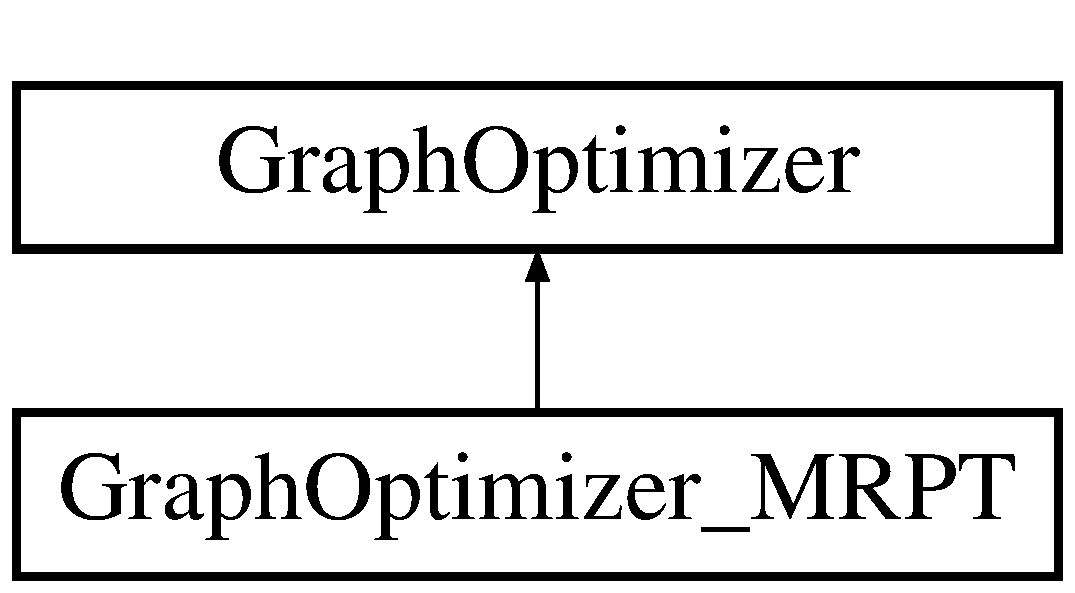
\includegraphics[height=2.000000cm]{class_graph_optimizer___m_r_p_t}
\end{center}
\end{figure}
\subsection*{Public Member Functions}
\begin{DoxyCompactItemize}
\item 
int \hyperlink{class_graph_optimizer___m_r_p_t_a2c5a89fce928859445d3ec2627a0ed3e}{addVertex} (Eigen::Matrix4f \&pose)
\item 
void \hyperlink{class_graph_optimizer___m_r_p_t_a593e4c3752d6e3b6340145e5fd03ad92}{addEdge} (const int fromIdx, const int toIdx, Eigen::Matrix4f \&relPose, Eigen::Matrix$<$ double, 6, 6 $>$ \&infMatrix)
\item 
void \hyperlink{class_graph_optimizer___m_r_p_t_aa60e33c3028018515f01aaae20ec9bd5}{optimizeGraph} ()
\item 
void \hyperlink{class_graph_optimizer___m_r_p_t_a40f1548815f2830a950bb682782793b7}{getPoses} (std::vector$<$ Eigen::Matrix4f, Eigen::aligned\_\-allocator$<$ Eigen::Matrix4f $>$ $>$ \&)
\item 
void \hyperlink{class_graph_optimizer___m_r_p_t_a5456297ea1d91e7cafc55e3a46ee7ad6}{saveGraph} (std::string fileName)
\end{DoxyCompactItemize}
\subsection*{Private Attributes}
\begin{DoxyCompactItemize}
\item 
\hypertarget{class_graph_optimizer___m_r_p_t_af1f16e6edcf0bff4861e940c3ab5987b}{
int {\bfseries vertexIdx}}
\label{class_graph_optimizer___m_r_p_t_af1f16e6edcf0bff4861e940c3ab5987b}

\item 
\hypertarget{class_graph_optimizer___m_r_p_t_aa0edf72c3742a01b7fc87130346a349b}{
mrpt::graphs::CNetworkOfPoses3DInf {\bfseries graph}}
\label{class_graph_optimizer___m_r_p_t_aa0edf72c3742a01b7fc87130346a349b}

\end{DoxyCompactItemize}


\subsection{Detailed Description}
This class encapsulates the functionality of the MRPT graph-\/slam module to perform 6D graph optimization. 

\subsection{Member Function Documentation}
\hypertarget{class_graph_optimizer___m_r_p_t_a593e4c3752d6e3b6340145e5fd03ad92}{
\index{GraphOptimizer\_\-MRPT@{GraphOptimizer\_\-MRPT}!addEdge@{addEdge}}
\index{addEdge@{addEdge}!GraphOptimizer_MRPT@{GraphOptimizer\_\-MRPT}}
\subsubsection[{addEdge}]{\setlength{\rightskip}{0pt plus 5cm}void GraphOptimizer\_\-MRPT::addEdge (
\begin{DoxyParamCaption}
\item[{const int}]{fromIdx, }
\item[{const int}]{toIdx, }
\item[{Eigen::Matrix4f \&}]{relPose, }
\item[{Eigen::Matrix$<$ double, 6, 6 $>$ \&}]{infMatrix}
\end{DoxyParamCaption}
)\hspace{0.3cm}{\ttfamily  \mbox{[}virtual\mbox{]}}}}
\label{class_graph_optimizer___m_r_p_t_a593e4c3752d6e3b6340145e5fd03ad92}
Adds an edge that defines a spatial constraint between the vertices \char`\"{}fromIdx\char`\"{} and \char`\"{}toIdx\char`\"{} with information matrix that determines the weight of the added edge. 

Implements \hyperlink{class_graph_optimizer_a7bf9e4c2d3376bf8af5b15c86398950e}{GraphOptimizer}.

\hypertarget{class_graph_optimizer___m_r_p_t_a2c5a89fce928859445d3ec2627a0ed3e}{
\index{GraphOptimizer\_\-MRPT@{GraphOptimizer\_\-MRPT}!addVertex@{addVertex}}
\index{addVertex@{addVertex}!GraphOptimizer_MRPT@{GraphOptimizer\_\-MRPT}}
\subsubsection[{addVertex}]{\setlength{\rightskip}{0pt plus 5cm}int GraphOptimizer\_\-MRPT::addVertex (
\begin{DoxyParamCaption}
\item[{Eigen::Matrix4f \&}]{pose}
\end{DoxyParamCaption}
)\hspace{0.3cm}{\ttfamily  \mbox{[}virtual\mbox{]}}}}
\label{class_graph_optimizer___m_r_p_t_a2c5a89fce928859445d3ec2627a0ed3e}
Adds a new vertex to the graph. The provided 4x4 matrix will be considered as the pose of the new added vertex. It returns the index of the added vertex. 

Implements \hyperlink{class_graph_optimizer_a2acd85307e0c0a006a2360f9d7e29bce}{GraphOptimizer}.

\hypertarget{class_graph_optimizer___m_r_p_t_a40f1548815f2830a950bb682782793b7}{
\index{GraphOptimizer\_\-MRPT@{GraphOptimizer\_\-MRPT}!getPoses@{getPoses}}
\index{getPoses@{getPoses}!GraphOptimizer_MRPT@{GraphOptimizer\_\-MRPT}}
\subsubsection[{getPoses}]{\setlength{\rightskip}{0pt plus 5cm}void GraphOptimizer\_\-MRPT::getPoses (
\begin{DoxyParamCaption}
\item[{std::vector$<$ Eigen::Matrix4f, Eigen::aligned\_\-allocator$<$ Eigen::Matrix4f $>$ $>$ \&}]{}
\end{DoxyParamCaption}
)\hspace{0.3cm}{\ttfamily  \mbox{[}virtual\mbox{]}}}}
\label{class_graph_optimizer___m_r_p_t_a40f1548815f2830a950bb682782793b7}
Returns a vector with all the optimized poses of the graph. 

Implements \hyperlink{class_graph_optimizer_a914f6c37de8dc6437122b3f563cce9a5}{GraphOptimizer}.

\hypertarget{class_graph_optimizer___m_r_p_t_aa60e33c3028018515f01aaae20ec9bd5}{
\index{GraphOptimizer\_\-MRPT@{GraphOptimizer\_\-MRPT}!optimizeGraph@{optimizeGraph}}
\index{optimizeGraph@{optimizeGraph}!GraphOptimizer_MRPT@{GraphOptimizer\_\-MRPT}}
\subsubsection[{optimizeGraph}]{\setlength{\rightskip}{0pt plus 5cm}void GraphOptimizer\_\-MRPT::optimizeGraph (
\begin{DoxyParamCaption}
{}
\end{DoxyParamCaption}
)\hspace{0.3cm}{\ttfamily  \mbox{[}virtual\mbox{]}}}}
\label{class_graph_optimizer___m_r_p_t_aa60e33c3028018515f01aaae20ec9bd5}
Calls the graph optimization process to determine the pose configuration that best satisfies the constraints defined by the edges. 

Implements \hyperlink{class_graph_optimizer_ad1e8ac7c0aa9c90f3035c1d29036eedb}{GraphOptimizer}.

\hypertarget{class_graph_optimizer___m_r_p_t_a5456297ea1d91e7cafc55e3a46ee7ad6}{
\index{GraphOptimizer\_\-MRPT@{GraphOptimizer\_\-MRPT}!saveGraph@{saveGraph}}
\index{saveGraph@{saveGraph}!GraphOptimizer_MRPT@{GraphOptimizer\_\-MRPT}}
\subsubsection[{saveGraph}]{\setlength{\rightskip}{0pt plus 5cm}void GraphOptimizer\_\-MRPT::saveGraph (
\begin{DoxyParamCaption}
\item[{std::string}]{fileName}
\end{DoxyParamCaption}
)\hspace{0.3cm}{\ttfamily  \mbox{[}virtual\mbox{]}}}}
\label{class_graph_optimizer___m_r_p_t_a5456297ea1d91e7cafc55e3a46ee7ad6}
Saves the graph to file. 

Implements \hyperlink{class_graph_optimizer_a303a1e4e96fa44433ef48aa4051fab32}{GraphOptimizer}.



The documentation for this class was generated from the following file:\begin{DoxyCompactItemize}
\item 
GraphOptimizer\_\-MRPT.h\end{DoxyCompactItemize}

\hypertarget{class_i_c_p_pose_refiner}{
\section{ICPPoseRefiner Class Reference}
\label{class_i_c_p_pose_refiner}\index{ICPPoseRefiner@{ICPPoseRefiner}}
}


{\ttfamily \#include $<$ICPPoseRefiner.h$>$}

Inheritance diagram for ICPPoseRefiner:\begin{figure}[H]
\begin{center}
\leavevmode
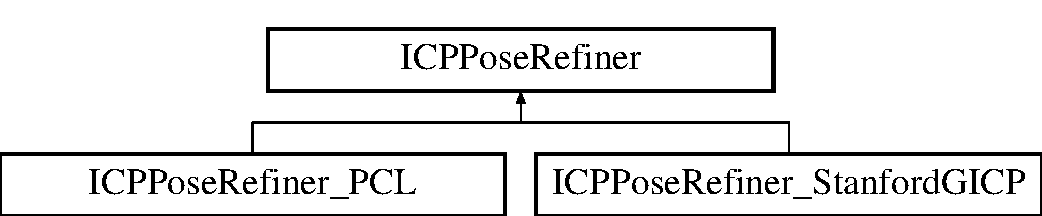
\includegraphics[height=2.000000cm]{class_i_c_p_pose_refiner}
\end{center}
\end{figure}
\subsection*{Public Member Functions}
\begin{DoxyCompactItemize}
\item 
virtual void \hyperlink{class_i_c_p_pose_refiner_ad359ab15346aa343a51bd8ae71cd3ea1}{refinePose} (\hyperlink{class_frame_r_g_b_d}{FrameRGBD} \&frame1, \hyperlink{class_frame_r_g_b_d}{FrameRGBD} \&frame2, Eigen::Matrix4f \&H)=0
\end{DoxyCompactItemize}


\subsection{Detailed Description}
Abstract class that defines a method to refine the rigid transformation between two RGBD frames using an ICP approach. 

\subsection{Member Function Documentation}
\hypertarget{class_i_c_p_pose_refiner_ad359ab15346aa343a51bd8ae71cd3ea1}{
\index{ICPPoseRefiner@{ICPPoseRefiner}!refinePose@{refinePose}}
\index{refinePose@{refinePose}!ICPPoseRefiner@{ICPPoseRefiner}}
\subsubsection[{refinePose}]{\setlength{\rightskip}{0pt plus 5cm}virtual void ICPPoseRefiner::refinePose (
\begin{DoxyParamCaption}
\item[{{\bf FrameRGBD} \&}]{frame1, }
\item[{{\bf FrameRGBD} \&}]{frame2, }
\item[{Eigen::Matrix4f \&}]{H}
\end{DoxyParamCaption}
)\hspace{0.3cm}{\ttfamily  \mbox{[}pure virtual\mbox{]}}}}
\label{class_i_c_p_pose_refiner_ad359ab15346aa343a51bd8ae71cd3ea1}
This method refines the 3D rigid transformation between frame1 and frame2 giving H as an initial guess. The refined rigid transformation will be returned in H. 

Implemented in \hyperlink{class_i_c_p_pose_refiner___p_c_l_a0efdc4657c30bf0a171b0a012f4f0d8d}{ICPPoseRefiner\_\-PCL}, and \hyperlink{class_i_c_p_pose_refiner___stanford_g_i_c_p_a943bad0b2578cf87723ce968e8c52580}{ICPPoseRefiner\_\-StanfordGICP}.



The documentation for this class was generated from the following file:\begin{DoxyCompactItemize}
\item 
ICPPoseRefiner.h\end{DoxyCompactItemize}

\hypertarget{class_i_c_p_pose_refiner___p_c_l}{
\section{ICPPoseRefiner\_\-PCL Class Reference}
\label{class_i_c_p_pose_refiner___p_c_l}\index{ICPPoseRefiner\_\-PCL@{ICPPoseRefiner\_\-PCL}}
}


{\ttfamily \#include $<$ICPPoseRefiner\_\-PCL.h$>$}

Inheritance diagram for ICPPoseRefiner\_\-PCL:\begin{figure}[H]
\begin{center}
\leavevmode
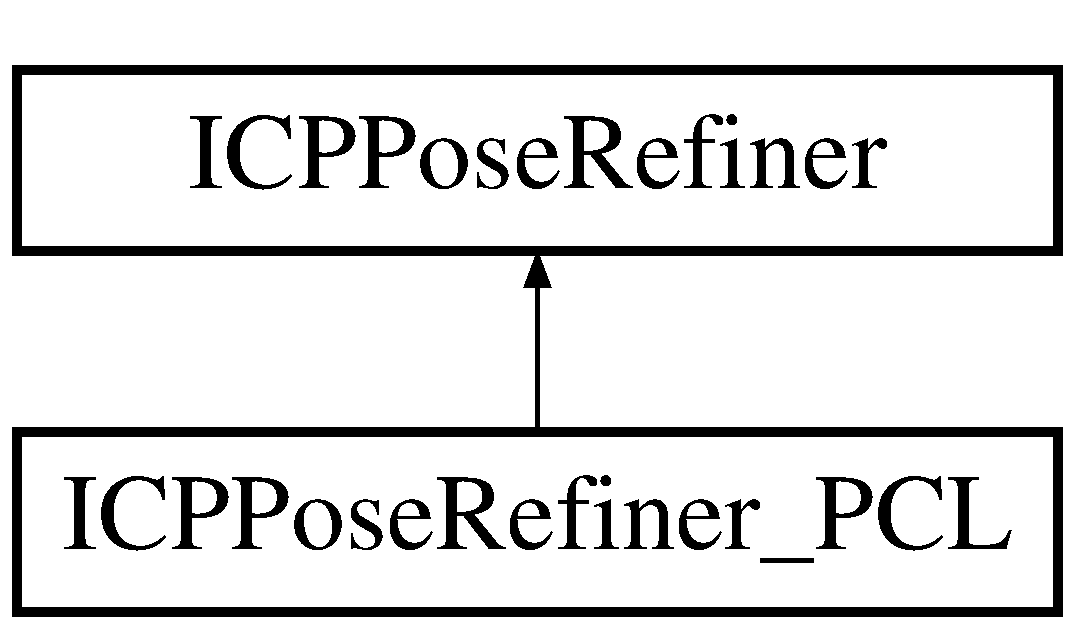
\includegraphics[height=2.000000cm]{class_i_c_p_pose_refiner___p_c_l}
\end{center}
\end{figure}
\subsection*{Public Member Functions}
\begin{DoxyCompactItemize}
\item 
void \hyperlink{class_i_c_p_pose_refiner___p_c_l_a0efdc4657c30bf0a171b0a012f4f0d8d}{refinePose} (\hyperlink{class_frame_r_g_b_d}{FrameRGBD} \&frame1, \hyperlink{class_frame_r_g_b_d}{FrameRGBD} \&frame2, Eigen::Matrix4f \&H)
\end{DoxyCompactItemize}
\subsection*{Private Attributes}
\begin{DoxyCompactItemize}
\item 
\hypertarget{class_i_c_p_pose_refiner___p_c_l_a18dee09c2029e84f6a1e72910c528662}{
pcl::IterativeClosestPoint$<$ pcl::PointXYZRGB, pcl::PointXYZRGB $>$ {\bfseries icp}}
\label{class_i_c_p_pose_refiner___p_c_l_a18dee09c2029e84f6a1e72910c528662}

\item 
\hypertarget{class_i_c_p_pose_refiner___p_c_l_a25d56d3d98d851da532f29215d9c930e}{
pcl::PointCloud$<$ pcl::PointXYZRGB $>$ {\bfseries alignedCloudPtr}}
\label{class_i_c_p_pose_refiner___p_c_l_a25d56d3d98d851da532f29215d9c930e}

\item 
\hypertarget{class_i_c_p_pose_refiner___p_c_l_acab3758cb1d71c76f5868fdef2e53f5a}{
float {\bfseries maxCorrespondenceDistance}}
\label{class_i_c_p_pose_refiner___p_c_l_acab3758cb1d71c76f5868fdef2e53f5a}

\item 
\hypertarget{class_i_c_p_pose_refiner___p_c_l_ac50c9d45d78f75561e8d978f0b297502}{
int {\bfseries maximumIterations}}
\label{class_i_c_p_pose_refiner___p_c_l_ac50c9d45d78f75561e8d978f0b297502}

\item 
\hypertarget{class_i_c_p_pose_refiner___p_c_l_a640d703fc7c39b86287e37b555b1db9b}{
float {\bfseries transformationEpsilon}}
\label{class_i_c_p_pose_refiner___p_c_l_a640d703fc7c39b86287e37b555b1db9b}

\end{DoxyCompactItemize}


\subsection{Detailed Description}
This class encapsulates the functionality of a 3D rigid transformation refiner using the standard ICP algorithm implemented in the PCL library. 

\subsection{Member Function Documentation}
\hypertarget{class_i_c_p_pose_refiner___p_c_l_a0efdc4657c30bf0a171b0a012f4f0d8d}{
\index{ICPPoseRefiner\_\-PCL@{ICPPoseRefiner\_\-PCL}!refinePose@{refinePose}}
\index{refinePose@{refinePose}!ICPPoseRefiner_PCL@{ICPPoseRefiner\_\-PCL}}
\subsubsection[{refinePose}]{\setlength{\rightskip}{0pt plus 5cm}void ICPPoseRefiner\_\-PCL::refinePose (
\begin{DoxyParamCaption}
\item[{{\bf FrameRGBD} \&}]{frame1, }
\item[{{\bf FrameRGBD} \&}]{frame2, }
\item[{Eigen::Matrix4f \&}]{H}
\end{DoxyParamCaption}
)\hspace{0.3cm}{\ttfamily  \mbox{[}virtual\mbox{]}}}}
\label{class_i_c_p_pose_refiner___p_c_l_a0efdc4657c30bf0a171b0a012f4f0d8d}
This method refines the 3D rigid transformation between frame1 and frame2 giving H as an initial guess. The refined rigid transformation will be returned in H. 

Implements \hyperlink{class_i_c_p_pose_refiner_ad359ab15346aa343a51bd8ae71cd3ea1}{ICPPoseRefiner}.



The documentation for this class was generated from the following file:\begin{DoxyCompactItemize}
\item 
ICPPoseRefiner\_\-PCL.h\end{DoxyCompactItemize}

\hypertarget{class_i_c_p_pose_refiner___stanford_g_i_c_p}{
\section{ICPPoseRefiner\_\-StanfordGICP Class Reference}
\label{class_i_c_p_pose_refiner___stanford_g_i_c_p}\index{ICPPoseRefiner\_\-StanfordGICP@{ICPPoseRefiner\_\-StanfordGICP}}
}


{\ttfamily \#include $<$ICPPoseRefiner\_\-StanfordGICP.h$>$}

Inheritance diagram for ICPPoseRefiner\_\-StanfordGICP:\begin{figure}[H]
\begin{center}
\leavevmode
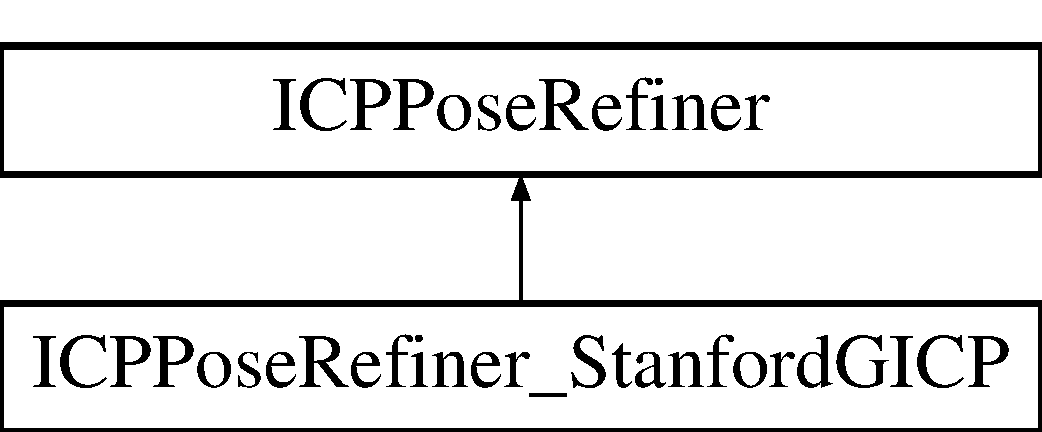
\includegraphics[height=2.000000cm]{class_i_c_p_pose_refiner___stanford_g_i_c_p}
\end{center}
\end{figure}
\subsection*{Public Member Functions}
\begin{DoxyCompactItemize}
\item 
void \hyperlink{class_i_c_p_pose_refiner___stanford_g_i_c_p_a943bad0b2578cf87723ce968e8c52580}{refinePose} (\hyperlink{class_frame_r_g_b_d}{FrameRGBD} \&frame1, \hyperlink{class_frame_r_g_b_d}{FrameRGBD} \&frame2, Eigen::Matrix4f \&H)
\end{DoxyCompactItemize}
\subsection*{Private Attributes}
\begin{DoxyCompactItemize}
\item 
\hypertarget{class_i_c_p_pose_refiner___stanford_g_i_c_p_a89681c536d6d4907cdaa8ab0d30f5728}{
bool {\bfseries debug}}
\label{class_i_c_p_pose_refiner___stanford_g_i_c_p_a89681c536d6d4907cdaa8ab0d30f5728}

\item 
\hypertarget{class_i_c_p_pose_refiner___stanford_g_i_c_p_a8e42ad076b05c36552d0e704ee156976}{
double {\bfseries gicp\_\-epsilon}}
\label{class_i_c_p_pose_refiner___stanford_g_i_c_p_a8e42ad076b05c36552d0e704ee156976}

\item 
\hypertarget{class_i_c_p_pose_refiner___stanford_g_i_c_p_ac4efce272acf7630f58e60d3b6629cea}{
double {\bfseries max\_\-distance}}
\label{class_i_c_p_pose_refiner___stanford_g_i_c_p_ac4efce272acf7630f58e60d3b6629cea}

\item 
\hypertarget{class_i_c_p_pose_refiner___stanford_g_i_c_p_a415c953f2b86d6b4433322d4ac57bf3a}{
GICPPointSet {\bfseries gicpPointSet1}}
\label{class_i_c_p_pose_refiner___stanford_g_i_c_p_a415c953f2b86d6b4433322d4ac57bf3a}

\item 
\hypertarget{class_i_c_p_pose_refiner___stanford_g_i_c_p_a894be0011b387374fa6f50ce5706d81e}{
GICPPointSet {\bfseries gicpPointSet2}}
\label{class_i_c_p_pose_refiner___stanford_g_i_c_p_a894be0011b387374fa6f50ce5706d81e}

\end{DoxyCompactItemize}


\subsection{Detailed Description}
This class encapsulates the functionality of a 3D rigid transformation refiner using the Generalized ICP algorithm implemented in the Stanford GICP library. The source code of the GICP library could be found here: \href{http://www.stanford.edu/~avsegal/generalized_icp.html}{\tt http://www.stanford.edu/$\sim$avsegal/generalized\_\-icp.html} 

\subsection{Member Function Documentation}
\hypertarget{class_i_c_p_pose_refiner___stanford_g_i_c_p_a943bad0b2578cf87723ce968e8c52580}{
\index{ICPPoseRefiner\_\-StanfordGICP@{ICPPoseRefiner\_\-StanfordGICP}!refinePose@{refinePose}}
\index{refinePose@{refinePose}!ICPPoseRefiner_StanfordGICP@{ICPPoseRefiner\_\-StanfordGICP}}
\subsubsection[{refinePose}]{\setlength{\rightskip}{0pt plus 5cm}void ICPPoseRefiner\_\-StanfordGICP::refinePose (
\begin{DoxyParamCaption}
\item[{{\bf FrameRGBD} \&}]{frame1, }
\item[{{\bf FrameRGBD} \&}]{frame2, }
\item[{Eigen::Matrix4f \&}]{H}
\end{DoxyParamCaption}
)\hspace{0.3cm}{\ttfamily  \mbox{[}virtual\mbox{]}}}}
\label{class_i_c_p_pose_refiner___stanford_g_i_c_p_a943bad0b2578cf87723ce968e8c52580}
This method refines the 3D rigid transformation between frame1 and frame2 giving H as an initial guess. The refined rigid transformation will be returned in H. 

Implements \hyperlink{class_i_c_p_pose_refiner_ad359ab15346aa343a51bd8ae71cd3ea1}{ICPPoseRefiner}.



The documentation for this class was generated from the following file:\begin{DoxyCompactItemize}
\item 
ICPPoseRefiner\_\-StanfordGICP.h\end{DoxyCompactItemize}

\hypertarget{class_keyframe_loop_detector}{
\section{KeyframeLoopDetector Class Reference}
\label{class_keyframe_loop_detector}\index{KeyframeLoopDetector@{KeyframeLoopDetector}}
}


{\ttfamily \#include $<$KeyframeLoopDetector.h$>$}

\subsection*{Public Member Functions}
\begin{DoxyCompactItemize}
\item 
\hypertarget{class_keyframe_loop_detector_a2b059bd8fa4faab0af9c4b6af835ec7b}{
{\bfseries KeyframeLoopDetector} (const int=30)}
\label{class_keyframe_loop_detector_a2b059bd8fa4faab0af9c4b6af835ec7b}

\item 
void \hyperlink{class_keyframe_loop_detector_a5ef5a7ee9dde3e1dd875a5c952dee85b}{addKeyframe} (\hyperlink{class_frame_r_g_b_d}{FrameRGBD} $\ast$keyframe)
\item 
void \hyperlink{class_keyframe_loop_detector_af3d4e5a2dfb91c1f461952fb32b0c366}{addPose} (Eigen::Matrix4f \&pose)
\item 
void \hyperlink{class_keyframe_loop_detector_ac5c7855ada4a3660902f535a309b5394}{addKeypoints} (std::vector$<$ cv::KeyPoint $>$ \&keypoints)
\item 
void \hyperlink{class_keyframe_loop_detector_adad3db780d35efdb3c27bf3bc92c12eb}{addDescriptors} (cv::Mat \&descriptors)
\item 
void \hyperlink{class_keyframe_loop_detector_a9f171abd08e32c09d0db76725f027261}{detectLoop} (\hyperlink{class_visual_feature_matcher___generic}{VisualFeatureMatcher\_\-Generic} \&matcher, \hyperlink{class_visual3_d_rigid_transformation_estimator}{Visual3DRigidTransformationEstimator} \&rigidTransformEstimator, \hyperlink{class_i_c_p_pose_refiner}{ICPPoseRefiner} \&poseRefiner, std::vector$<$ Eigen::Matrix4f, Eigen::aligned\_\-allocator$<$ Eigen::Matrix4f $>$ $>$ \&relativePoses, std::vector$<$ Eigen::Matrix$<$ double, 6, 6 $>$, Eigen::aligned\_\-allocator$<$ Eigen::Matrix$<$ double, 6, 6 $>$ $>$ $>$ \&infMatrices, std::vector$<$ int $>$ \&fromIndexes, int \&toIndex)
\item 
void \hyperlink{class_keyframe_loop_detector_a5b5a6c7378ab3846693c9d0025b7aa37}{getPoses} (std::vector$<$ Eigen::Matrix4f, Eigen::aligned\_\-allocator$<$ Eigen::Matrix4f $>$ $>$ \&)
\item 
void \hyperlink{class_keyframe_loop_detector_a7043fa83b96b7407d4b4d31610574afe}{getKeyframes} (std::vector$<$ \hyperlink{class_frame_r_g_b_d}{FrameRGBD} $\ast$ $>$ \&)
\item 
void \hyperlink{class_keyframe_loop_detector_aa9b5a576a6c1a696840b3aeb208f2e40}{accumulateRelativePose} (Eigen::Matrix4f \&relPose)
\item 
void \hyperlink{class_keyframe_loop_detector_afce6712ebcfabb34d34b7917b7f18ea9}{getCurrentPose} (Eigen::Matrix4f \&pose)
\item 
void \hyperlink{class_keyframe_loop_detector_af4d7c5e2e9404d63197077c67fca0662}{setPoses} (std::vector$<$ Eigen::Matrix4f, Eigen::aligned\_\-allocator$<$ Eigen::Matrix4f $>$ $>$ \&)
\item 
void \hyperlink{class_keyframe_loop_detector_af4cdff4bb98bd31b5a16347cff2da072}{saveLoopProfiling} (std::string fileName)
\end{DoxyCompactItemize}
\subsection*{Private Attributes}
\begin{DoxyCompactItemize}
\item 
std::vector$<$ \hyperlink{class_frame_r_g_b_d}{FrameRGBD} $\ast$ $>$ \hyperlink{class_keyframe_loop_detector_a9fc839f91a21d9666dbf40610d2be7df}{keyframes}
\item 
std::vector$<$ Eigen::Matrix4f, Eigen::aligned\_\-allocator$<$ Eigen::Matrix4f $>$ $>$ \hyperlink{class_keyframe_loop_detector_a486f9714c66706b85febede7f3653676}{poses}
\item 
std::vector$<$ std::vector$<$ cv::KeyPoint $>$ $>$ \hyperlink{class_keyframe_loop_detector_aed3185bed2b9c9c1e342d155f370bc60}{keypointsList}
\item 
std::vector$<$ cv::Mat $>$ \hyperlink{class_keyframe_loop_detector_a523e7cacd0a93ce8bc5a55100c571bed}{descriptorsList}
\item 
int \hyperlink{class_keyframe_loop_detector_a88bfa794730e06898b2f9aede72f22ca}{numberInliersThreshold}
\item 
\hypertarget{class_keyframe_loop_detector_a86cd4a82b86a5ebdce90bccda946bcc2}{
Eigen::Matrix4f {\bfseries relativePose}}
\label{class_keyframe_loop_detector_a86cd4a82b86a5ebdce90bccda946bcc2}

\item 
\hypertarget{class_keyframe_loop_detector_a8b48f2156c77ecb7822365016454fb16}{
mrpt::utils::CTimeLogger {\bfseries profiler}}
\label{class_keyframe_loop_detector_a8b48f2156c77ecb7822365016454fb16}

\end{DoxyCompactItemize}


\subsection{Detailed Description}
This class implements a very straightforward approach for loop detection. It is based on the resulting number of inliers from the feature matching process. This implementation matches the last added keyframe against all the previous keyframes to find the ones that best match. If the number of inliers are greater than a certain threshold, then it considers that both the matched previous keyframe and the current keyframe belongs to the same place (loop detection). This class returns not only the loops between keyframes, but also the spatial constraints between keyframes. 

\subsection{Member Function Documentation}
\hypertarget{class_keyframe_loop_detector_aa9b5a576a6c1a696840b3aeb208f2e40}{
\index{KeyframeLoopDetector@{KeyframeLoopDetector}!accumulateRelativePose@{accumulateRelativePose}}
\index{accumulateRelativePose@{accumulateRelativePose}!KeyframeLoopDetector@{KeyframeLoopDetector}}
\subsubsection[{accumulateRelativePose}]{\setlength{\rightskip}{0pt plus 5cm}void KeyframeLoopDetector::accumulateRelativePose (
\begin{DoxyParamCaption}
\item[{Eigen::Matrix4f \&}]{relPose}
\end{DoxyParamCaption}
)}}
\label{class_keyframe_loop_detector_aa9b5a576a6c1a696840b3aeb208f2e40}
Adds a new pose accumulating the provided relative pose. \hypertarget{class_keyframe_loop_detector_adad3db780d35efdb3c27bf3bc92c12eb}{
\index{KeyframeLoopDetector@{KeyframeLoopDetector}!addDescriptors@{addDescriptors}}
\index{addDescriptors@{addDescriptors}!KeyframeLoopDetector@{KeyframeLoopDetector}}
\subsubsection[{addDescriptors}]{\setlength{\rightskip}{0pt plus 5cm}void KeyframeLoopDetector::addDescriptors (
\begin{DoxyParamCaption}
\item[{cv::Mat \&}]{descriptors}
\end{DoxyParamCaption}
)}}
\label{class_keyframe_loop_detector_adad3db780d35efdb3c27bf3bc92c12eb}
Adds the descriptors corresponding to the keypoints of the added keyframe. \hypertarget{class_keyframe_loop_detector_a5ef5a7ee9dde3e1dd875a5c952dee85b}{
\index{KeyframeLoopDetector@{KeyframeLoopDetector}!addKeyframe@{addKeyframe}}
\index{addKeyframe@{addKeyframe}!KeyframeLoopDetector@{KeyframeLoopDetector}}
\subsubsection[{addKeyframe}]{\setlength{\rightskip}{0pt plus 5cm}void KeyframeLoopDetector::addKeyframe (
\begin{DoxyParamCaption}
\item[{{\bf FrameRGBD} $\ast$}]{keyframe}
\end{DoxyParamCaption}
)}}
\label{class_keyframe_loop_detector_a5ef5a7ee9dde3e1dd875a5c952dee85b}
Adds a new keyframe to the loop detector. \hypertarget{class_keyframe_loop_detector_ac5c7855ada4a3660902f535a309b5394}{
\index{KeyframeLoopDetector@{KeyframeLoopDetector}!addKeypoints@{addKeypoints}}
\index{addKeypoints@{addKeypoints}!KeyframeLoopDetector@{KeyframeLoopDetector}}
\subsubsection[{addKeypoints}]{\setlength{\rightskip}{0pt plus 5cm}void KeyframeLoopDetector::addKeypoints (
\begin{DoxyParamCaption}
\item[{std::vector$<$ cv::KeyPoint $>$ \&}]{keypoints}
\end{DoxyParamCaption}
)}}
\label{class_keyframe_loop_detector_ac5c7855ada4a3660902f535a309b5394}
Adds the keypoints corresponding the intensity image of the added keyframe. \hypertarget{class_keyframe_loop_detector_af3d4e5a2dfb91c1f461952fb32b0c366}{
\index{KeyframeLoopDetector@{KeyframeLoopDetector}!addPose@{addPose}}
\index{addPose@{addPose}!KeyframeLoopDetector@{KeyframeLoopDetector}}
\subsubsection[{addPose}]{\setlength{\rightskip}{0pt plus 5cm}void KeyframeLoopDetector::addPose (
\begin{DoxyParamCaption}
\item[{Eigen::Matrix4f \&}]{pose}
\end{DoxyParamCaption}
)}}
\label{class_keyframe_loop_detector_af3d4e5a2dfb91c1f461952fb32b0c366}
Adds a 6D pose that specifies the position and orientation of the camera from which the keyframe has been grabbed. \hypertarget{class_keyframe_loop_detector_a9f171abd08e32c09d0db76725f027261}{
\index{KeyframeLoopDetector@{KeyframeLoopDetector}!detectLoop@{detectLoop}}
\index{detectLoop@{detectLoop}!KeyframeLoopDetector@{KeyframeLoopDetector}}
\subsubsection[{detectLoop}]{\setlength{\rightskip}{0pt plus 5cm}void KeyframeLoopDetector::detectLoop (
\begin{DoxyParamCaption}
\item[{{\bf VisualFeatureMatcher\_\-Generic} \&}]{matcher, }
\item[{{\bf Visual3DRigidTransformationEstimator} \&}]{rigidTransformEstimator, }
\item[{{\bf ICPPoseRefiner} \&}]{poseRefiner, }
\item[{std::vector$<$ Eigen::Matrix4f, Eigen::aligned\_\-allocator$<$ Eigen::Matrix4f $>$ $>$ \&}]{relativePoses, }
\item[{std::vector$<$ Eigen::Matrix$<$ double, 6, 6 $>$, Eigen::aligned\_\-allocator$<$ Eigen::Matrix$<$ double, 6, 6 $>$ $>$ $>$ \&}]{infMatrices, }
\item[{std::vector$<$ int $>$ \&}]{fromIndexes, }
\item[{int \&}]{toIndex}
\end{DoxyParamCaption}
)}}
\label{class_keyframe_loop_detector_a9f171abd08e32c09d0db76725f027261}
Performs the loop detection process matching the added keyframe against previous keyframes. It returns a vector of 6D relatives poses that defines spatial constraints between keyframes, a vector of 6x6 information matrices that represents the goodness of the matches. It also returns a vector of keyframe indexes and a keyframe index that determines the \char`\"{}origins\char`\"{} and \char`\"{}end\char`\"{} of each loop. \hypertarget{class_keyframe_loop_detector_afce6712ebcfabb34d34b7917b7f18ea9}{
\index{KeyframeLoopDetector@{KeyframeLoopDetector}!getCurrentPose@{getCurrentPose}}
\index{getCurrentPose@{getCurrentPose}!KeyframeLoopDetector@{KeyframeLoopDetector}}
\subsubsection[{getCurrentPose}]{\setlength{\rightskip}{0pt plus 5cm}void KeyframeLoopDetector::getCurrentPose (
\begin{DoxyParamCaption}
\item[{Eigen::Matrix4f \&}]{pose}
\end{DoxyParamCaption}
)}}
\label{class_keyframe_loop_detector_afce6712ebcfabb34d34b7917b7f18ea9}
Returns the current keyframe pose. \hypertarget{class_keyframe_loop_detector_a7043fa83b96b7407d4b4d31610574afe}{
\index{KeyframeLoopDetector@{KeyframeLoopDetector}!getKeyframes@{getKeyframes}}
\index{getKeyframes@{getKeyframes}!KeyframeLoopDetector@{KeyframeLoopDetector}}
\subsubsection[{getKeyframes}]{\setlength{\rightskip}{0pt plus 5cm}void KeyframeLoopDetector::getKeyframes (
\begin{DoxyParamCaption}
\item[{std::vector$<$ {\bf FrameRGBD} $\ast$ $>$ \&}]{}
\end{DoxyParamCaption}
)}}
\label{class_keyframe_loop_detector_a7043fa83b96b7407d4b4d31610574afe}
Returns a vector of all the keyframes \hypertarget{class_keyframe_loop_detector_a5b5a6c7378ab3846693c9d0025b7aa37}{
\index{KeyframeLoopDetector@{KeyframeLoopDetector}!getPoses@{getPoses}}
\index{getPoses@{getPoses}!KeyframeLoopDetector@{KeyframeLoopDetector}}
\subsubsection[{getPoses}]{\setlength{\rightskip}{0pt plus 5cm}void KeyframeLoopDetector::getPoses (
\begin{DoxyParamCaption}
\item[{std::vector$<$ Eigen::Matrix4f, Eigen::aligned\_\-allocator$<$ Eigen::Matrix4f $>$ $>$ \&}]{}
\end{DoxyParamCaption}
)}}
\label{class_keyframe_loop_detector_a5b5a6c7378ab3846693c9d0025b7aa37}
Returns a vector of all the keyframe poses. \hypertarget{class_keyframe_loop_detector_af4cdff4bb98bd31b5a16347cff2da072}{
\index{KeyframeLoopDetector@{KeyframeLoopDetector}!saveLoopProfiling@{saveLoopProfiling}}
\index{saveLoopProfiling@{saveLoopProfiling}!KeyframeLoopDetector@{KeyframeLoopDetector}}
\subsubsection[{saveLoopProfiling}]{\setlength{\rightskip}{0pt plus 5cm}void KeyframeLoopDetector::saveLoopProfiling (
\begin{DoxyParamCaption}
\item[{std::string}]{fileName}
\end{DoxyParamCaption}
)}}
\label{class_keyframe_loop_detector_af4cdff4bb98bd31b5a16347cff2da072}
Save profiling results for loop detection \hypertarget{class_keyframe_loop_detector_af4d7c5e2e9404d63197077c67fca0662}{
\index{KeyframeLoopDetector@{KeyframeLoopDetector}!setPoses@{setPoses}}
\index{setPoses@{setPoses}!KeyframeLoopDetector@{KeyframeLoopDetector}}
\subsubsection[{setPoses}]{\setlength{\rightskip}{0pt plus 5cm}void KeyframeLoopDetector::setPoses (
\begin{DoxyParamCaption}
\item[{std::vector$<$ Eigen::Matrix4f, Eigen::aligned\_\-allocator$<$ Eigen::Matrix4f $>$ $>$ \&}]{}
\end{DoxyParamCaption}
)}}
\label{class_keyframe_loop_detector_af4d7c5e2e9404d63197077c67fca0662}
Sets the vector of keyframe poses with the provided vector of poses. 

\subsection{Field Documentation}
\hypertarget{class_keyframe_loop_detector_a523e7cacd0a93ce8bc5a55100c571bed}{
\index{KeyframeLoopDetector@{KeyframeLoopDetector}!descriptorsList@{descriptorsList}}
\index{descriptorsList@{descriptorsList}!KeyframeLoopDetector@{KeyframeLoopDetector}}
\subsubsection[{descriptorsList}]{\setlength{\rightskip}{0pt plus 5cm}std::vector$<$cv::Mat$>$ {\bf KeyframeLoopDetector::descriptorsList}\hspace{0.3cm}{\ttfamily  \mbox{[}private\mbox{]}}}}
\label{class_keyframe_loop_detector_a523e7cacd0a93ce8bc5a55100c571bed}
Vector of the decriptors corresponding to the 2D keypoints of each keyframe. \hypertarget{class_keyframe_loop_detector_a9fc839f91a21d9666dbf40610d2be7df}{
\index{KeyframeLoopDetector@{KeyframeLoopDetector}!keyframes@{keyframes}}
\index{keyframes@{keyframes}!KeyframeLoopDetector@{KeyframeLoopDetector}}
\subsubsection[{keyframes}]{\setlength{\rightskip}{0pt plus 5cm}std::vector$<${\bf FrameRGBD}$\ast$$>$ {\bf KeyframeLoopDetector::keyframes}\hspace{0.3cm}{\ttfamily  \mbox{[}private\mbox{]}}}}
\label{class_keyframe_loop_detector_a9fc839f91a21d9666dbf40610d2be7df}
Vector of all the added keyframes. \hypertarget{class_keyframe_loop_detector_aed3185bed2b9c9c1e342d155f370bc60}{
\index{KeyframeLoopDetector@{KeyframeLoopDetector}!keypointsList@{keypointsList}}
\index{keypointsList@{keypointsList}!KeyframeLoopDetector@{KeyframeLoopDetector}}
\subsubsection[{keypointsList}]{\setlength{\rightskip}{0pt plus 5cm}std::vector$<$std::vector$<$cv::KeyPoint$>$ $>$ {\bf KeyframeLoopDetector::keypointsList}\hspace{0.3cm}{\ttfamily  \mbox{[}private\mbox{]}}}}
\label{class_keyframe_loop_detector_aed3185bed2b9c9c1e342d155f370bc60}
Vector of the 2D keypoints corresponding to the intensity image of each keyframe. \hypertarget{class_keyframe_loop_detector_a88bfa794730e06898b2f9aede72f22ca}{
\index{KeyframeLoopDetector@{KeyframeLoopDetector}!numberInliersThreshold@{numberInliersThreshold}}
\index{numberInliersThreshold@{numberInliersThreshold}!KeyframeLoopDetector@{KeyframeLoopDetector}}
\subsubsection[{numberInliersThreshold}]{\setlength{\rightskip}{0pt plus 5cm}int {\bf KeyframeLoopDetector::numberInliersThreshold}\hspace{0.3cm}{\ttfamily  \mbox{[}private\mbox{]}}}}
\label{class_keyframe_loop_detector_a88bfa794730e06898b2f9aede72f22ca}
Threshold that specifies the minimum number of inliers needed to detect a loop. \hypertarget{class_keyframe_loop_detector_a486f9714c66706b85febede7f3653676}{
\index{KeyframeLoopDetector@{KeyframeLoopDetector}!poses@{poses}}
\index{poses@{poses}!KeyframeLoopDetector@{KeyframeLoopDetector}}
\subsubsection[{poses}]{\setlength{\rightskip}{0pt plus 5cm}std::vector$<$Eigen::Matrix4f, Eigen::aligned\_\-allocator$<$Eigen::Matrix4f $>$ $>$ {\bf KeyframeLoopDetector::poses}\hspace{0.3cm}{\ttfamily  \mbox{[}private\mbox{]}}}}
\label{class_keyframe_loop_detector_a486f9714c66706b85febede7f3653676}
Vector of the 6D poses corresponding to each keyframe. 

The documentation for this class was generated from the following file:\begin{DoxyCompactItemize}
\item 
KeyframeLoopDetector.h\end{DoxyCompactItemize}

\hypertarget{class_kinect_grabber}{
\section{KinectGrabber Class Reference}
\label{class_kinect_grabber}\index{KinectGrabber@{KinectGrabber}}
}


{\ttfamily \#include $<$KinectGrabber.h$>$}

Inheritance diagram for KinectGrabber:\begin{figure}[H]
\begin{center}
\leavevmode
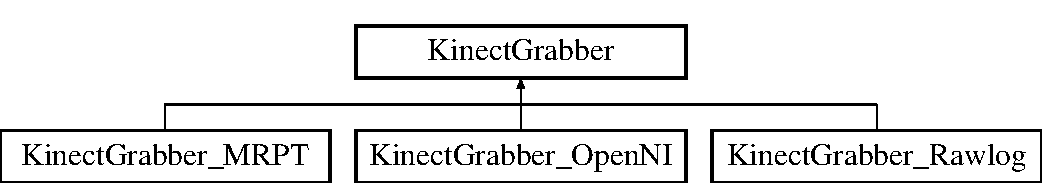
\includegraphics[height=2.000000cm]{class_kinect_grabber}
\end{center}
\end{figure}
\subsection*{Public Member Functions}
\begin{DoxyCompactItemize}
\item 
virtual void \hyperlink{class_kinect_grabber_a053e560dfd15e6123d19e4aa20b19585}{getCurrentColouredPointCloudPtr} (pcl::PointCloud$<$ pcl::PointXYZRGB $>$::Ptr \&colouredPointCloudPtr)=0
\item 
virtual void \hyperlink{class_kinect_grabber_a3faafcbdbb136dd2c6b51d51eed9e147}{filterPointCloud} (pcl::PointCloud$<$ pcl::PointXYZRGB $>$::Ptr \&colouredPointCloudPtr, pcl::PointCloud$<$ pcl::PointXYZRGB $>$::Ptr \&downsampledPointCloudPtr)=0
\item 
virtual void \hyperlink{class_kinect_grabber_a47a54afb0a188cdd02f3cf79d503b3dd}{getCurrentIntensityImage} (cv::Mat \&intensityImage)=0
\item 
virtual void \hyperlink{class_kinect_grabber_a0274f336f9aee07bca08bd673cf9377a}{grab} ()=0
\item 
virtual void \hyperlink{class_kinect_grabber_af7d0fcdc2f85f84cb38469095882d688}{stopGrabber} ()=0
\item 
virtual void \hyperlink{class_kinect_grabber_abca25bbc3ddc8bc99dc1c84df48ae9f2}{getCurrentFrameRGBD} (\hyperlink{class_frame_r_g_b_d}{FrameRGBD} \&)=0
\end{DoxyCompactItemize}
\subsection*{Protected Member Functions}
\begin{DoxyCompactItemize}
\item 
\hypertarget{class_kinect_grabber_aa3e6643ea33d0cbf53ed6b8b67689730}{
void {\bfseries initPointCloudDownsampler} ()}
\label{class_kinect_grabber_aa3e6643ea33d0cbf53ed6b8b67689730}

\end{DoxyCompactItemize}
\subsection*{Protected Attributes}
\begin{DoxyCompactItemize}
\item 
\hypertarget{class_kinect_grabber_aca653c8782e67efdbf7460892325546f}{
pcl::PointCloud$<$ pcl::PointXYZRGB $>$::Ptr {\bfseries currentColouredPointCloudPtr}}
\label{class_kinect_grabber_aca653c8782e67efdbf7460892325546f}

\item 
\hypertarget{class_kinect_grabber_a9b1dfc42f58f60187958dcddd26fb951}{
pcl::PointCloud$<$ pcl::PointXYZRGB $>$::Ptr {\bfseries currentDownsampledPointCloudPtr}}
\label{class_kinect_grabber_a9b1dfc42f58f60187958dcddd26fb951}

\item 
\hypertarget{class_kinect_grabber_a4d3713b372fe44cfbb3c0a6d05a82474}{
cv::Mat {\bfseries currentIntensityImage}}
\label{class_kinect_grabber_a4d3713b372fe44cfbb3c0a6d05a82474}

\item 
\hypertarget{class_kinect_grabber_a4008d163b78268910c6e1550eaeb7f8f}{
\hyperlink{class_point_cloud_downsampler}{PointCloudDownsampler} {\bfseries grid}}
\label{class_kinect_grabber_a4008d163b78268910c6e1550eaeb7f8f}

\end{DoxyCompactItemize}


\subsection{Detailed Description}
Abstract class \hyperlink{class_kinect_grabber}{KinectGrabber} that especifies the functionality of a generic RGBD grabber. This class especifies methods to grab a \hyperlink{class_frame_r_g_b_d}{FrameRGBD} and stop grabbing. 

\subsection{Member Function Documentation}
\hypertarget{class_kinect_grabber_a3faafcbdbb136dd2c6b51d51eed9e147}{
\index{KinectGrabber@{KinectGrabber}!filterPointCloud@{filterPointCloud}}
\index{filterPointCloud@{filterPointCloud}!KinectGrabber@{KinectGrabber}}
\subsubsection[{filterPointCloud}]{\setlength{\rightskip}{0pt plus 5cm}virtual void KinectGrabber::filterPointCloud (
\begin{DoxyParamCaption}
\item[{pcl::PointCloud$<$ pcl::PointXYZRGB $>$::Ptr \&}]{colouredPointCloudPtr, }
\item[{pcl::PointCloud$<$ pcl::PointXYZRGB $>$::Ptr \&}]{downsampledPointCloudPtr}
\end{DoxyParamCaption}
)\hspace{0.3cm}{\ttfamily  \mbox{[}pure virtual\mbox{]}}}}
\label{class_kinect_grabber_a3faafcbdbb136dd2c6b51d51eed9e147}
Returns a downsampled version of the provided 3D point cloud. 

Implemented in \hyperlink{class_kinect_grabber___m_r_p_t_acd8b9e162fa31c4f1940fbea6bdd9669}{KinectGrabber\_\-MRPT}, \hyperlink{class_kinect_grabber___open_n_i_a6f3449aae89913eaa1ce2f1d82f2e80c}{KinectGrabber\_\-OpenNI}, and \hyperlink{class_kinect_grabber___rawlog_a91322ecfdf2706e9fa160679e49c9960}{KinectGrabber\_\-Rawlog}.

\hypertarget{class_kinect_grabber_a053e560dfd15e6123d19e4aa20b19585}{
\index{KinectGrabber@{KinectGrabber}!getCurrentColouredPointCloudPtr@{getCurrentColouredPointCloudPtr}}
\index{getCurrentColouredPointCloudPtr@{getCurrentColouredPointCloudPtr}!KinectGrabber@{KinectGrabber}}
\subsubsection[{getCurrentColouredPointCloudPtr}]{\setlength{\rightskip}{0pt plus 5cm}virtual void KinectGrabber::getCurrentColouredPointCloudPtr (
\begin{DoxyParamCaption}
\item[{pcl::PointCloud$<$ pcl::PointXYZRGB $>$::Ptr \&}]{colouredPointCloudPtr}
\end{DoxyParamCaption}
)\hspace{0.3cm}{\ttfamily  \mbox{[}pure virtual\mbox{]}}}}
\label{class_kinect_grabber_a053e560dfd15e6123d19e4aa20b19585}
Returns the current 3D coloured point cloud. 

Implemented in \hyperlink{class_kinect_grabber___m_r_p_t_a11aee26f0e640ca8b43f629b838a43a9}{KinectGrabber\_\-MRPT}, \hyperlink{class_kinect_grabber___open_n_i_a49fcf8f7d6160a72cae3a8c69663412d}{KinectGrabber\_\-OpenNI}, and \hyperlink{class_kinect_grabber___rawlog_a111bd24662e2dcf4ab3ee82a26a089b6}{KinectGrabber\_\-Rawlog}.

\hypertarget{class_kinect_grabber_abca25bbc3ddc8bc99dc1c84df48ae9f2}{
\index{KinectGrabber@{KinectGrabber}!getCurrentFrameRGBD@{getCurrentFrameRGBD}}
\index{getCurrentFrameRGBD@{getCurrentFrameRGBD}!KinectGrabber@{KinectGrabber}}
\subsubsection[{getCurrentFrameRGBD}]{\setlength{\rightskip}{0pt plus 5cm}virtual void KinectGrabber::getCurrentFrameRGBD (
\begin{DoxyParamCaption}
\item[{{\bf FrameRGBD} \&}]{}
\end{DoxyParamCaption}
)\hspace{0.3cm}{\ttfamily  \mbox{[}pure virtual\mbox{]}}}}
\label{class_kinect_grabber_abca25bbc3ddc8bc99dc1c84df48ae9f2}
Returns a RGBD frame containing the intensity image and 3D point cloud. It also computes a downsampled version of the 3D point cloud and adds it to the returned RGBD frame. 

Implemented in \hyperlink{class_kinect_grabber___m_r_p_t_a64ec507059096493aa6c1c172b31b651}{KinectGrabber\_\-MRPT}, \hyperlink{class_kinect_grabber___open_n_i_ac85fcc37d21dcd74066af85bf055d66b}{KinectGrabber\_\-OpenNI}, and \hyperlink{class_kinect_grabber___rawlog_aa5633577a641a2f4f22dcc92bae059c3}{KinectGrabber\_\-Rawlog}.

\hypertarget{class_kinect_grabber_a47a54afb0a188cdd02f3cf79d503b3dd}{
\index{KinectGrabber@{KinectGrabber}!getCurrentIntensityImage@{getCurrentIntensityImage}}
\index{getCurrentIntensityImage@{getCurrentIntensityImage}!KinectGrabber@{KinectGrabber}}
\subsubsection[{getCurrentIntensityImage}]{\setlength{\rightskip}{0pt plus 5cm}virtual void KinectGrabber::getCurrentIntensityImage (
\begin{DoxyParamCaption}
\item[{cv::Mat \&}]{intensityImage}
\end{DoxyParamCaption}
)\hspace{0.3cm}{\ttfamily  \mbox{[}pure virtual\mbox{]}}}}
\label{class_kinect_grabber_a47a54afb0a188cdd02f3cf79d503b3dd}
Returns the current intensity image provided by the RGB camera. 

Implemented in \hyperlink{class_kinect_grabber___m_r_p_t_adf243a3557ff0347c7eee98c0c2a309b}{KinectGrabber\_\-MRPT}, \hyperlink{class_kinect_grabber___open_n_i_ab06b4b2825042c47facb5a10697b114e}{KinectGrabber\_\-OpenNI}, and \hyperlink{class_kinect_grabber___rawlog_aa3f3757bb08b3453661084e1439c73e6}{KinectGrabber\_\-Rawlog}.

\hypertarget{class_kinect_grabber_a0274f336f9aee07bca08bd673cf9377a}{
\index{KinectGrabber@{KinectGrabber}!grab@{grab}}
\index{grab@{grab}!KinectGrabber@{KinectGrabber}}
\subsubsection[{grab}]{\setlength{\rightskip}{0pt plus 5cm}virtual void KinectGrabber::grab (
\begin{DoxyParamCaption}
{}
\end{DoxyParamCaption}
)\hspace{0.3cm}{\ttfamily  \mbox{[}pure virtual\mbox{]}}}}
\label{class_kinect_grabber_a0274f336f9aee07bca08bd673cf9377a}
Retains the current intensity image and its corresponding 3D point cloud. 

Implemented in \hyperlink{class_kinect_grabber___m_r_p_t_ac5997c6197eed0f9bd0977f45a5d5928}{KinectGrabber\_\-MRPT}, \hyperlink{class_kinect_grabber___open_n_i_a75b04004b7cfa8a061fbadae7825ade4}{KinectGrabber\_\-OpenNI}, and \hyperlink{class_kinect_grabber___rawlog_a1eac54348c1963bd5823337b72e10583}{KinectGrabber\_\-Rawlog}.

\hypertarget{class_kinect_grabber_af7d0fcdc2f85f84cb38469095882d688}{
\index{KinectGrabber@{KinectGrabber}!stopGrabber@{stopGrabber}}
\index{stopGrabber@{stopGrabber}!KinectGrabber@{KinectGrabber}}
\subsubsection[{stopGrabber}]{\setlength{\rightskip}{0pt plus 5cm}virtual void KinectGrabber::stopGrabber (
\begin{DoxyParamCaption}
{}
\end{DoxyParamCaption}
)\hspace{0.3cm}{\ttfamily  \mbox{[}pure virtual\mbox{]}}}}
\label{class_kinect_grabber_af7d0fcdc2f85f84cb38469095882d688}
Stop grabing RGBD frames. 

Implemented in \hyperlink{class_kinect_grabber___m_r_p_t_a9fee110b324eab5a7e852509643a101f}{KinectGrabber\_\-MRPT}, \hyperlink{class_kinect_grabber___open_n_i_a5618f02db9a2b8e514bdee738c472ba3}{KinectGrabber\_\-OpenNI}, and \hyperlink{class_kinect_grabber___rawlog_a17b718e8d4142965a84f8bedad738834}{KinectGrabber\_\-Rawlog}.



The documentation for this class was generated from the following file:\begin{DoxyCompactItemize}
\item 
KinectGrabber.h\end{DoxyCompactItemize}

\hypertarget{class_kinect_grabber___m_r_p_t}{
\section{KinectGrabber\_\-MRPT Class Reference}
\label{class_kinect_grabber___m_r_p_t}\index{KinectGrabber\_\-MRPT@{KinectGrabber\_\-MRPT}}
}


{\ttfamily \#include $<$KinectGrabber\_\-MRPT.h$>$}

Inheritance diagram for KinectGrabber\_\-MRPT:\begin{figure}[H]
\begin{center}
\leavevmode
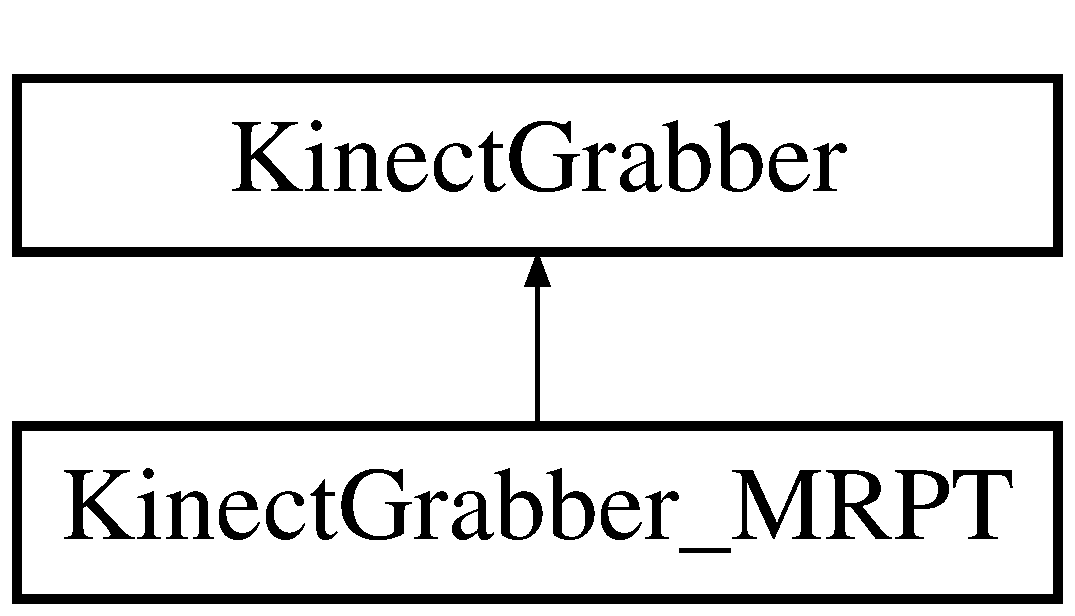
\includegraphics[height=2.000000cm]{class_kinect_grabber___m_r_p_t}
\end{center}
\end{figure}
\subsection*{Data Structures}
\begin{DoxyCompactItemize}
\item 
struct \hyperlink{struct_kinect_grabber___m_r_p_t_1_1_t_thread_param}{TThreadParam}
\end{DoxyCompactItemize}
\subsection*{Public Member Functions}
\begin{DoxyCompactItemize}
\item 
void \hyperlink{class_kinect_grabber___m_r_p_t_a11aee26f0e640ca8b43f629b838a43a9}{getCurrentColouredPointCloudPtr} (pcl::PointCloud$<$ pcl::PointXYZRGB $>$::Ptr \&colouredPointCloudPtr)
\item 
void \hyperlink{class_kinect_grabber___m_r_p_t_acd8b9e162fa31c4f1940fbea6bdd9669}{filterPointCloud} (pcl::PointCloud$<$ pcl::PointXYZRGB $>$::Ptr \&colouredPointCloudPtr, pcl::PointCloud$<$ pcl::PointXYZRGB $>$::Ptr \&downsampledPointCloudPtr)
\item 
void \hyperlink{class_kinect_grabber___m_r_p_t_adf243a3557ff0347c7eee98c0c2a309b}{getCurrentIntensityImage} (cv::Mat \&intensityImage)
\item 
void \hyperlink{class_kinect_grabber___m_r_p_t_ac5997c6197eed0f9bd0977f45a5d5928}{grab} ()
\item 
void \hyperlink{class_kinect_grabber___m_r_p_t_a9fee110b324eab5a7e852509643a101f}{stopGrabber} ()
\item 
void \hyperlink{class_kinect_grabber___m_r_p_t_a64ec507059096493aa6c1c172b31b651}{getCurrentFrameRGBD} (\hyperlink{class_frame_r_g_b_d}{FrameRGBD} \&)
\end{DoxyCompactItemize}
\subsection*{Data Fields}
\begin{DoxyCompactItemize}
\item 
\hypertarget{class_kinect_grabber___m_r_p_t_ac5c832a0409b5da3777f0266e84ef978}{
\hyperlink{struct_kinect_grabber___m_r_p_t_1_1_t_thread_param}{TThreadParam} $\ast$ {\bfseries thrParPtr}}
\label{class_kinect_grabber___m_r_p_t_ac5c832a0409b5da3777f0266e84ef978}

\end{DoxyCompactItemize}
\subsection*{Private Attributes}
\begin{DoxyCompactItemize}
\item 
\hypertarget{class_kinect_grabber___m_r_p_t_a6c0a144f3022d3a63d13dc96e3f4458d}{
CObservation3DRangeScanPtr {\bfseries currentObservationPtr}}
\label{class_kinect_grabber___m_r_p_t_a6c0a144f3022d3a63d13dc96e3f4458d}

\item 
\hypertarget{class_kinect_grabber___m_r_p_t_aea9a7c992f3236da3c3b35acca25fdba}{
mrpt::system::TThreadHandle {\bfseries thHandle}}
\label{class_kinect_grabber___m_r_p_t_aea9a7c992f3236da3c3b35acca25fdba}

\end{DoxyCompactItemize}


\subsection{Detailed Description}
This class captures RGBD frames from the Kinect sensor using the MRPT library to access the sensor data. It grabs the intensity image as well as its corresponding 3D point cloud. 

\subsection{Member Function Documentation}
\hypertarget{class_kinect_grabber___m_r_p_t_acd8b9e162fa31c4f1940fbea6bdd9669}{
\index{KinectGrabber\_\-MRPT@{KinectGrabber\_\-MRPT}!filterPointCloud@{filterPointCloud}}
\index{filterPointCloud@{filterPointCloud}!KinectGrabber_MRPT@{KinectGrabber\_\-MRPT}}
\subsubsection[{filterPointCloud}]{\setlength{\rightskip}{0pt plus 5cm}void KinectGrabber\_\-MRPT::filterPointCloud (
\begin{DoxyParamCaption}
\item[{pcl::PointCloud$<$ pcl::PointXYZRGB $>$::Ptr \&}]{colouredPointCloudPtr, }
\item[{pcl::PointCloud$<$ pcl::PointXYZRGB $>$::Ptr \&}]{downsampledPointCloudPtr}
\end{DoxyParamCaption}
)\hspace{0.3cm}{\ttfamily  \mbox{[}virtual\mbox{]}}}}
\label{class_kinect_grabber___m_r_p_t_acd8b9e162fa31c4f1940fbea6bdd9669}
Returns a downsampled version of the provided 3D point cloud. 

Implements \hyperlink{class_kinect_grabber_a3faafcbdbb136dd2c6b51d51eed9e147}{KinectGrabber}.

\hypertarget{class_kinect_grabber___m_r_p_t_a11aee26f0e640ca8b43f629b838a43a9}{
\index{KinectGrabber\_\-MRPT@{KinectGrabber\_\-MRPT}!getCurrentColouredPointCloudPtr@{getCurrentColouredPointCloudPtr}}
\index{getCurrentColouredPointCloudPtr@{getCurrentColouredPointCloudPtr}!KinectGrabber_MRPT@{KinectGrabber\_\-MRPT}}
\subsubsection[{getCurrentColouredPointCloudPtr}]{\setlength{\rightskip}{0pt plus 5cm}void KinectGrabber\_\-MRPT::getCurrentColouredPointCloudPtr (
\begin{DoxyParamCaption}
\item[{pcl::PointCloud$<$ pcl::PointXYZRGB $>$::Ptr \&}]{colouredPointCloudPtr}
\end{DoxyParamCaption}
)\hspace{0.3cm}{\ttfamily  \mbox{[}virtual\mbox{]}}}}
\label{class_kinect_grabber___m_r_p_t_a11aee26f0e640ca8b43f629b838a43a9}
Returns the current 3D coloured point cloud. 

Implements \hyperlink{class_kinect_grabber_a053e560dfd15e6123d19e4aa20b19585}{KinectGrabber}.

\hypertarget{class_kinect_grabber___m_r_p_t_a64ec507059096493aa6c1c172b31b651}{
\index{KinectGrabber\_\-MRPT@{KinectGrabber\_\-MRPT}!getCurrentFrameRGBD@{getCurrentFrameRGBD}}
\index{getCurrentFrameRGBD@{getCurrentFrameRGBD}!KinectGrabber_MRPT@{KinectGrabber\_\-MRPT}}
\subsubsection[{getCurrentFrameRGBD}]{\setlength{\rightskip}{0pt plus 5cm}void KinectGrabber\_\-MRPT::getCurrentFrameRGBD (
\begin{DoxyParamCaption}
\item[{{\bf FrameRGBD} \&}]{}
\end{DoxyParamCaption}
)\hspace{0.3cm}{\ttfamily  \mbox{[}virtual\mbox{]}}}}
\label{class_kinect_grabber___m_r_p_t_a64ec507059096493aa6c1c172b31b651}
Returns a RGBD frame containing the intensity image and 3D point cloud. It also computes a downsampled version of the 3D point cloud and adds it to the returned RGBD frame. 

Implements \hyperlink{class_kinect_grabber_abca25bbc3ddc8bc99dc1c84df48ae9f2}{KinectGrabber}.

\hypertarget{class_kinect_grabber___m_r_p_t_adf243a3557ff0347c7eee98c0c2a309b}{
\index{KinectGrabber\_\-MRPT@{KinectGrabber\_\-MRPT}!getCurrentIntensityImage@{getCurrentIntensityImage}}
\index{getCurrentIntensityImage@{getCurrentIntensityImage}!KinectGrabber_MRPT@{KinectGrabber\_\-MRPT}}
\subsubsection[{getCurrentIntensityImage}]{\setlength{\rightskip}{0pt plus 5cm}void KinectGrabber\_\-MRPT::getCurrentIntensityImage (
\begin{DoxyParamCaption}
\item[{cv::Mat \&}]{intensityImage}
\end{DoxyParamCaption}
)\hspace{0.3cm}{\ttfamily  \mbox{[}virtual\mbox{]}}}}
\label{class_kinect_grabber___m_r_p_t_adf243a3557ff0347c7eee98c0c2a309b}
Returns the current intensity image provided by the RGB camera. 

Implements \hyperlink{class_kinect_grabber_a47a54afb0a188cdd02f3cf79d503b3dd}{KinectGrabber}.

\hypertarget{class_kinect_grabber___m_r_p_t_ac5997c6197eed0f9bd0977f45a5d5928}{
\index{KinectGrabber\_\-MRPT@{KinectGrabber\_\-MRPT}!grab@{grab}}
\index{grab@{grab}!KinectGrabber_MRPT@{KinectGrabber\_\-MRPT}}
\subsubsection[{grab}]{\setlength{\rightskip}{0pt plus 5cm}void KinectGrabber\_\-MRPT::grab (
\begin{DoxyParamCaption}
{}
\end{DoxyParamCaption}
)\hspace{0.3cm}{\ttfamily  \mbox{[}virtual\mbox{]}}}}
\label{class_kinect_grabber___m_r_p_t_ac5997c6197eed0f9bd0977f45a5d5928}
Retains the current intensity image and its corresponding 3D point cloud. 

Implements \hyperlink{class_kinect_grabber_a0274f336f9aee07bca08bd673cf9377a}{KinectGrabber}.

\hypertarget{class_kinect_grabber___m_r_p_t_a9fee110b324eab5a7e852509643a101f}{
\index{KinectGrabber\_\-MRPT@{KinectGrabber\_\-MRPT}!stopGrabber@{stopGrabber}}
\index{stopGrabber@{stopGrabber}!KinectGrabber_MRPT@{KinectGrabber\_\-MRPT}}
\subsubsection[{stopGrabber}]{\setlength{\rightskip}{0pt plus 5cm}void KinectGrabber\_\-MRPT::stopGrabber (
\begin{DoxyParamCaption}
{}
\end{DoxyParamCaption}
)\hspace{0.3cm}{\ttfamily  \mbox{[}virtual\mbox{]}}}}
\label{class_kinect_grabber___m_r_p_t_a9fee110b324eab5a7e852509643a101f}
Stop grabing RGBD frames. 

Implements \hyperlink{class_kinect_grabber_af7d0fcdc2f85f84cb38469095882d688}{KinectGrabber}.



The documentation for this class was generated from the following file:\begin{DoxyCompactItemize}
\item 
KinectGrabber\_\-MRPT.h\end{DoxyCompactItemize}

\hypertarget{class_kinect_grabber___open_n_i}{
\section{KinectGrabber\_\-OpenNI Class Reference}
\label{class_kinect_grabber___open_n_i}\index{KinectGrabber\_\-OpenNI@{KinectGrabber\_\-OpenNI}}
}


{\ttfamily \#include $<$KinectGrabber\_\-OpenNI.h$>$}

Inheritance diagram for KinectGrabber\_\-OpenNI:\begin{figure}[H]
\begin{center}
\leavevmode
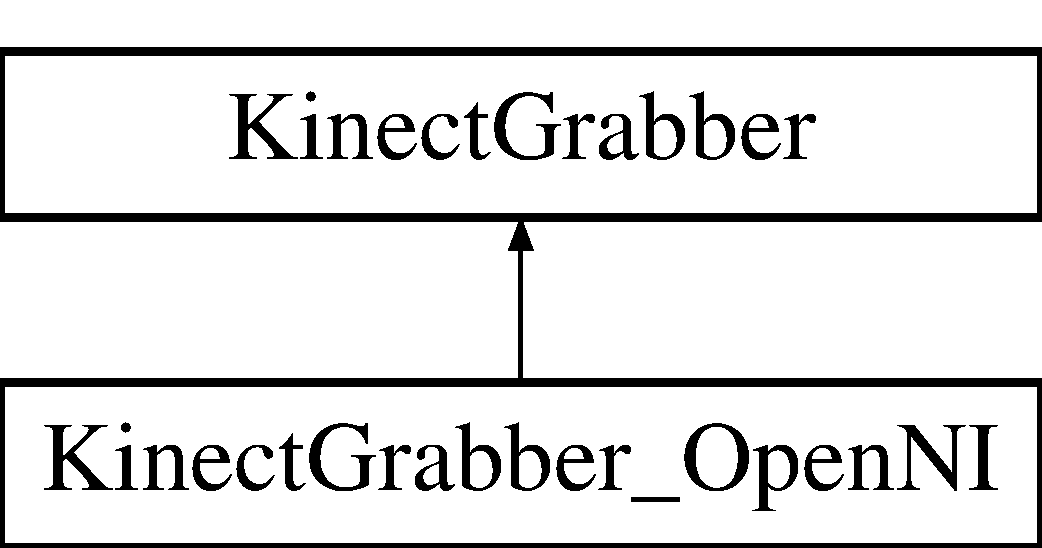
\includegraphics[height=2.000000cm]{class_kinect_grabber___open_n_i}
\end{center}
\end{figure}
\subsection*{Public Member Functions}
\begin{DoxyCompactItemize}
\item 
void \hyperlink{class_kinect_grabber___open_n_i_a49fcf8f7d6160a72cae3a8c69663412d}{getCurrentColouredPointCloudPtr} (pcl::PointCloud$<$ pcl::PointXYZRGB $>$::Ptr \&colouredPointCloudPtr)
\item 
void \hyperlink{class_kinect_grabber___open_n_i_a6f3449aae89913eaa1ce2f1d82f2e80c}{filterPointCloud} (pcl::PointCloud$<$ pcl::PointXYZRGB $>$::Ptr \&colouredPointCloudPtr, pcl::PointCloud$<$ pcl::PointXYZRGB $>$::Ptr \&downsampledPointCloudPtr)
\item 
void \hyperlink{class_kinect_grabber___open_n_i_ab06b4b2825042c47facb5a10697b114e}{getCurrentIntensityImage} (cv::Mat \&intensityImage)
\item 
void \hyperlink{class_kinect_grabber___open_n_i_a75b04004b7cfa8a061fbadae7825ade4}{grab} ()
\item 
void \hyperlink{class_kinect_grabber___open_n_i_a5618f02db9a2b8e514bdee738c472ba3}{stopGrabber} ()
\item 
void \hyperlink{class_kinect_grabber___open_n_i_ac85fcc37d21dcd74066af85bf055d66b}{getCurrentFrameRGBD} (\hyperlink{class_frame_r_g_b_d}{FrameRGBD} \&)
\end{DoxyCompactItemize}
\subsection*{Private Member Functions}
\begin{DoxyCompactItemize}
\item 
\hypertarget{class_kinect_grabber___open_n_i_a8ea8eb028145dab226c19ddaa0e154d4}{
void {\bfseries cloud\_\-cb\_\-} (const pcl::PointCloud$<$ pcl::PointXYZRGB $>$::ConstPtr \&cloud)}
\label{class_kinect_grabber___open_n_i_a8ea8eb028145dab226c19ddaa0e154d4}

\item 
\hypertarget{class_kinect_grabber___open_n_i_a13c87e25b183ff1d6d891fe771730ec5}{
void {\bfseries image\_\-cb\_\-} (const boost::shared\_\-ptr$<$ openni\_\-wrapper::Image $>$ \&img)}
\label{class_kinect_grabber___open_n_i_a13c87e25b183ff1d6d891fe771730ec5}

\end{DoxyCompactItemize}
\subsection*{Private Attributes}
\begin{DoxyCompactItemize}
\item 
\hypertarget{class_kinect_grabber___open_n_i_af9f188dc0939ceae194e99aec12a9e7b}{
cv::Mat {\bfseries currentRGBImg}}
\label{class_kinect_grabber___open_n_i_af9f188dc0939ceae194e99aec12a9e7b}

\item 
\hypertarget{class_kinect_grabber___open_n_i_a758bee0be65ad86d8f7c24d9fbb68cff}{
cv::Mat {\bfseries currentBGRImg}}
\label{class_kinect_grabber___open_n_i_a758bee0be65ad86d8f7c24d9fbb68cff}

\item 
\hypertarget{class_kinect_grabber___open_n_i_abaf74fe8bba94fab483e8b49745814dc}{
pcl::PointCloud$<$ pcl::PointXYZRGB $>$::ConstPtr {\bfseries pointCloudPtr\_\-aux}}
\label{class_kinect_grabber___open_n_i_abaf74fe8bba94fab483e8b49745814dc}

\item 
\hypertarget{class_kinect_grabber___open_n_i_a3a1075350645cea736211c6c34c136c8}{
pcl::OpenNIGrabber $\ast$ {\bfseries interface}}
\label{class_kinect_grabber___open_n_i_a3a1075350645cea736211c6c34c136c8}

\end{DoxyCompactItemize}


\subsection{Detailed Description}
This class captures RGBD frames from the Kinect sensor using the OpenNI interface provided by the PCL library to access the sensor data. It grabs the intensity image as well as its corresponding 3D point cloud. 

\subsection{Member Function Documentation}
\hypertarget{class_kinect_grabber___open_n_i_a6f3449aae89913eaa1ce2f1d82f2e80c}{
\index{KinectGrabber\_\-OpenNI@{KinectGrabber\_\-OpenNI}!filterPointCloud@{filterPointCloud}}
\index{filterPointCloud@{filterPointCloud}!KinectGrabber_OpenNI@{KinectGrabber\_\-OpenNI}}
\subsubsection[{filterPointCloud}]{\setlength{\rightskip}{0pt plus 5cm}void KinectGrabber\_\-OpenNI::filterPointCloud (
\begin{DoxyParamCaption}
\item[{pcl::PointCloud$<$ pcl::PointXYZRGB $>$::Ptr \&}]{colouredPointCloudPtr, }
\item[{pcl::PointCloud$<$ pcl::PointXYZRGB $>$::Ptr \&}]{downsampledPointCloudPtr}
\end{DoxyParamCaption}
)\hspace{0.3cm}{\ttfamily  \mbox{[}virtual\mbox{]}}}}
\label{class_kinect_grabber___open_n_i_a6f3449aae89913eaa1ce2f1d82f2e80c}
Returns a downsampled version of the provided 3D point cloud. 

Implements \hyperlink{class_kinect_grabber_a3faafcbdbb136dd2c6b51d51eed9e147}{KinectGrabber}.

\hypertarget{class_kinect_grabber___open_n_i_a49fcf8f7d6160a72cae3a8c69663412d}{
\index{KinectGrabber\_\-OpenNI@{KinectGrabber\_\-OpenNI}!getCurrentColouredPointCloudPtr@{getCurrentColouredPointCloudPtr}}
\index{getCurrentColouredPointCloudPtr@{getCurrentColouredPointCloudPtr}!KinectGrabber_OpenNI@{KinectGrabber\_\-OpenNI}}
\subsubsection[{getCurrentColouredPointCloudPtr}]{\setlength{\rightskip}{0pt plus 5cm}void KinectGrabber\_\-OpenNI::getCurrentColouredPointCloudPtr (
\begin{DoxyParamCaption}
\item[{pcl::PointCloud$<$ pcl::PointXYZRGB $>$::Ptr \&}]{colouredPointCloudPtr}
\end{DoxyParamCaption}
)\hspace{0.3cm}{\ttfamily  \mbox{[}virtual\mbox{]}}}}
\label{class_kinect_grabber___open_n_i_a49fcf8f7d6160a72cae3a8c69663412d}
Returns the current 3D coloured point cloud. 

Implements \hyperlink{class_kinect_grabber_a053e560dfd15e6123d19e4aa20b19585}{KinectGrabber}.

\hypertarget{class_kinect_grabber___open_n_i_ac85fcc37d21dcd74066af85bf055d66b}{
\index{KinectGrabber\_\-OpenNI@{KinectGrabber\_\-OpenNI}!getCurrentFrameRGBD@{getCurrentFrameRGBD}}
\index{getCurrentFrameRGBD@{getCurrentFrameRGBD}!KinectGrabber_OpenNI@{KinectGrabber\_\-OpenNI}}
\subsubsection[{getCurrentFrameRGBD}]{\setlength{\rightskip}{0pt plus 5cm}void KinectGrabber\_\-OpenNI::getCurrentFrameRGBD (
\begin{DoxyParamCaption}
\item[{{\bf FrameRGBD} \&}]{}
\end{DoxyParamCaption}
)\hspace{0.3cm}{\ttfamily  \mbox{[}virtual\mbox{]}}}}
\label{class_kinect_grabber___open_n_i_ac85fcc37d21dcd74066af85bf055d66b}
Returns a RGBD frame containing the intensity image and 3D point cloud. It also computes a downsampled version of the 3D point cloud and adds it to the returned RGBD frame. 

Implements \hyperlink{class_kinect_grabber_abca25bbc3ddc8bc99dc1c84df48ae9f2}{KinectGrabber}.

\hypertarget{class_kinect_grabber___open_n_i_ab06b4b2825042c47facb5a10697b114e}{
\index{KinectGrabber\_\-OpenNI@{KinectGrabber\_\-OpenNI}!getCurrentIntensityImage@{getCurrentIntensityImage}}
\index{getCurrentIntensityImage@{getCurrentIntensityImage}!KinectGrabber_OpenNI@{KinectGrabber\_\-OpenNI}}
\subsubsection[{getCurrentIntensityImage}]{\setlength{\rightskip}{0pt plus 5cm}void KinectGrabber\_\-OpenNI::getCurrentIntensityImage (
\begin{DoxyParamCaption}
\item[{cv::Mat \&}]{intensityImage}
\end{DoxyParamCaption}
)\hspace{0.3cm}{\ttfamily  \mbox{[}virtual\mbox{]}}}}
\label{class_kinect_grabber___open_n_i_ab06b4b2825042c47facb5a10697b114e}
Returns the current intensity image provided by the RGB camera. 

Implements \hyperlink{class_kinect_grabber_a47a54afb0a188cdd02f3cf79d503b3dd}{KinectGrabber}.

\hypertarget{class_kinect_grabber___open_n_i_a75b04004b7cfa8a061fbadae7825ade4}{
\index{KinectGrabber\_\-OpenNI@{KinectGrabber\_\-OpenNI}!grab@{grab}}
\index{grab@{grab}!KinectGrabber_OpenNI@{KinectGrabber\_\-OpenNI}}
\subsubsection[{grab}]{\setlength{\rightskip}{0pt plus 5cm}void KinectGrabber\_\-OpenNI::grab (
\begin{DoxyParamCaption}
{}
\end{DoxyParamCaption}
)\hspace{0.3cm}{\ttfamily  \mbox{[}virtual\mbox{]}}}}
\label{class_kinect_grabber___open_n_i_a75b04004b7cfa8a061fbadae7825ade4}
Retains the current intensity image and its corresponding 3D point cloud. 

Implements \hyperlink{class_kinect_grabber_a0274f336f9aee07bca08bd673cf9377a}{KinectGrabber}.

\hypertarget{class_kinect_grabber___open_n_i_a5618f02db9a2b8e514bdee738c472ba3}{
\index{KinectGrabber\_\-OpenNI@{KinectGrabber\_\-OpenNI}!stopGrabber@{stopGrabber}}
\index{stopGrabber@{stopGrabber}!KinectGrabber_OpenNI@{KinectGrabber\_\-OpenNI}}
\subsubsection[{stopGrabber}]{\setlength{\rightskip}{0pt plus 5cm}void KinectGrabber\_\-OpenNI::stopGrabber (
\begin{DoxyParamCaption}
{}
\end{DoxyParamCaption}
)\hspace{0.3cm}{\ttfamily  \mbox{[}virtual\mbox{]}}}}
\label{class_kinect_grabber___open_n_i_a5618f02db9a2b8e514bdee738c472ba3}
Stop grabing RGBD frames. 

Implements \hyperlink{class_kinect_grabber_af7d0fcdc2f85f84cb38469095882d688}{KinectGrabber}.



The documentation for this class was generated from the following file:\begin{DoxyCompactItemize}
\item 
KinectGrabber\_\-OpenNI.h\end{DoxyCompactItemize}

\hypertarget{class_kinect_grabber___rawlog}{
\section{KinectGrabber\_\-Rawlog Class Reference}
\label{class_kinect_grabber___rawlog}\index{KinectGrabber\_\-Rawlog@{KinectGrabber\_\-Rawlog}}
}


{\ttfamily \#include $<$KinectGrabber\_\-Rawlog.h$>$}

Inheritance diagram for KinectGrabber\_\-Rawlog:\begin{figure}[H]
\begin{center}
\leavevmode
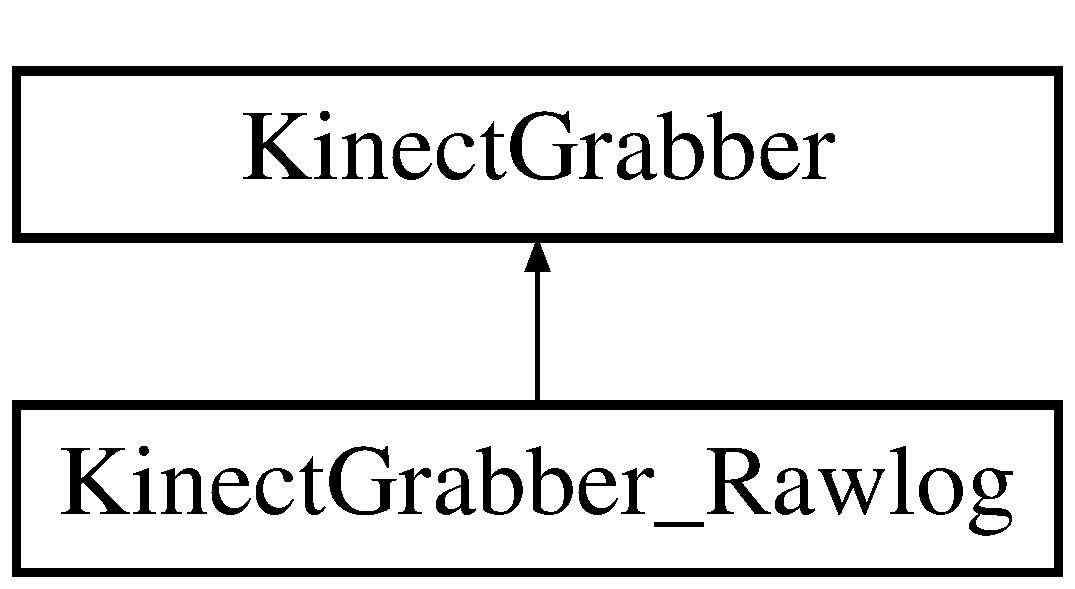
\includegraphics[height=2.000000cm]{class_kinect_grabber___rawlog}
\end{center}
\end{figure}
\subsection*{Data Structures}
\begin{DoxyCompactItemize}
\item 
struct \hyperlink{struct_kinect_grabber___rawlog_1_1_t_thread_param}{TThreadParam}
\end{DoxyCompactItemize}
\subsection*{Public Member Functions}
\begin{DoxyCompactItemize}
\item 
\hyperlink{class_kinect_grabber___rawlog_abd7e578bb31953eb6e2eb39543319f62}{KinectGrabber\_\-Rawlog} (const std::string \&rawlog\_\-file)
\item 
void \hyperlink{class_kinect_grabber___rawlog_a111bd24662e2dcf4ab3ee82a26a089b6}{getCurrentColouredPointCloudPtr} (pcl::PointCloud$<$ pcl::PointXYZRGB $>$::Ptr \&colouredPointCloudPtr)
\item 
void \hyperlink{class_kinect_grabber___rawlog_a91322ecfdf2706e9fa160679e49c9960}{filterPointCloud} (pcl::PointCloud$<$ pcl::PointXYZRGB $>$::Ptr \&colouredPointCloudPtr, pcl::PointCloud$<$ pcl::PointXYZRGB $>$::Ptr \&downsampledPointCloudPtr)
\item 
void \hyperlink{class_kinect_grabber___rawlog_aa3f3757bb08b3453661084e1439c73e6}{getCurrentIntensityImage} (cv::Mat \&intensityImage)
\item 
void \hyperlink{class_kinect_grabber___rawlog_a1eac54348c1963bd5823337b72e10583}{grab} ()
\item 
void \hyperlink{class_kinect_grabber___rawlog_a17b718e8d4142965a84f8bedad738834}{stopGrabber} ()
\item 
void \hyperlink{class_kinect_grabber___rawlog_aa5633577a641a2f4f22dcc92bae059c3}{getCurrentFrameRGBD} (\hyperlink{class_frame_r_g_b_d}{FrameRGBD} \&)
\end{DoxyCompactItemize}
\subsection*{Data Fields}
\begin{DoxyCompactItemize}
\item 
\hypertarget{class_kinect_grabber___rawlog_a7aa6e56a18c9090f2b3009ab691a4850}{
\hyperlink{struct_kinect_grabber___rawlog_1_1_t_thread_param}{TThreadParam} $\ast$ {\bfseries thrParPtr}}
\label{class_kinect_grabber___rawlog_a7aa6e56a18c9090f2b3009ab691a4850}

\end{DoxyCompactItemize}
\subsection*{Private Attributes}
\begin{DoxyCompactItemize}
\item 
\hypertarget{class_kinect_grabber___rawlog_a0f4c2d06f54de46bbe64df6435982b87}{
mrpt::slam::CObservation3DRangeScanPtr {\bfseries currentObservationPtr}}
\label{class_kinect_grabber___rawlog_a0f4c2d06f54de46bbe64df6435982b87}

\item 
\hypertarget{class_kinect_grabber___rawlog_acf419f440ab2a1c7e94a997004c066ff}{
mrpt::system::TThreadHandle {\bfseries thHandle}}
\label{class_kinect_grabber___rawlog_acf419f440ab2a1c7e94a997004c066ff}

\item 
\hypertarget{class_kinect_grabber___rawlog_a4b6bc22294bb13860292c0d5ddb7002e}{
mrpt::system::TTimeStamp {\bfseries timeStamp}}
\label{class_kinect_grabber___rawlog_a4b6bc22294bb13860292c0d5ddb7002e}

\end{DoxyCompactItemize}


\subsection{Detailed Description}
This class captures RGBD frames from rawlog sensor data using the MRPT library. It grabs the intensity image as well as its corresponding 3D point cloud. It also grabs the timestamp of each frame if provided in the rawlog. 

\subsection{Constructor \& Destructor Documentation}
\hypertarget{class_kinect_grabber___rawlog_abd7e578bb31953eb6e2eb39543319f62}{
\index{KinectGrabber\_\-Rawlog@{KinectGrabber\_\-Rawlog}!KinectGrabber\_\-Rawlog@{KinectGrabber\_\-Rawlog}}
\index{KinectGrabber\_\-Rawlog@{KinectGrabber\_\-Rawlog}!KinectGrabber_Rawlog@{KinectGrabber\_\-Rawlog}}
\subsubsection[{KinectGrabber\_\-Rawlog}]{\setlength{\rightskip}{0pt plus 5cm}KinectGrabber\_\-Rawlog::KinectGrabber\_\-Rawlog (
\begin{DoxyParamCaption}
\item[{const std::string \&}]{rawlog\_\-file}
\end{DoxyParamCaption}
)}}
\label{class_kinect_grabber___rawlog_abd7e578bb31953eb6e2eb39543319f62}
Creates a \hyperlink{class_kinect_grabber___rawlog}{KinectGrabber\_\-Rawlog} instance that grabs RGBD frames from the specified rawlog file. 

\subsection{Member Function Documentation}
\hypertarget{class_kinect_grabber___rawlog_a91322ecfdf2706e9fa160679e49c9960}{
\index{KinectGrabber\_\-Rawlog@{KinectGrabber\_\-Rawlog}!filterPointCloud@{filterPointCloud}}
\index{filterPointCloud@{filterPointCloud}!KinectGrabber_Rawlog@{KinectGrabber\_\-Rawlog}}
\subsubsection[{filterPointCloud}]{\setlength{\rightskip}{0pt plus 5cm}void KinectGrabber\_\-Rawlog::filterPointCloud (
\begin{DoxyParamCaption}
\item[{pcl::PointCloud$<$ pcl::PointXYZRGB $>$::Ptr \&}]{colouredPointCloudPtr, }
\item[{pcl::PointCloud$<$ pcl::PointXYZRGB $>$::Ptr \&}]{downsampledPointCloudPtr}
\end{DoxyParamCaption}
)\hspace{0.3cm}{\ttfamily  \mbox{[}virtual\mbox{]}}}}
\label{class_kinect_grabber___rawlog_a91322ecfdf2706e9fa160679e49c9960}
Returns a downsampled version of the provided 3D point cloud. 

Implements \hyperlink{class_kinect_grabber_a3faafcbdbb136dd2c6b51d51eed9e147}{KinectGrabber}.

\hypertarget{class_kinect_grabber___rawlog_a111bd24662e2dcf4ab3ee82a26a089b6}{
\index{KinectGrabber\_\-Rawlog@{KinectGrabber\_\-Rawlog}!getCurrentColouredPointCloudPtr@{getCurrentColouredPointCloudPtr}}
\index{getCurrentColouredPointCloudPtr@{getCurrentColouredPointCloudPtr}!KinectGrabber_Rawlog@{KinectGrabber\_\-Rawlog}}
\subsubsection[{getCurrentColouredPointCloudPtr}]{\setlength{\rightskip}{0pt plus 5cm}void KinectGrabber\_\-Rawlog::getCurrentColouredPointCloudPtr (
\begin{DoxyParamCaption}
\item[{pcl::PointCloud$<$ pcl::PointXYZRGB $>$::Ptr \&}]{colouredPointCloudPtr}
\end{DoxyParamCaption}
)\hspace{0.3cm}{\ttfamily  \mbox{[}virtual\mbox{]}}}}
\label{class_kinect_grabber___rawlog_a111bd24662e2dcf4ab3ee82a26a089b6}
Returns the current 3D coloured point cloud. 

Implements \hyperlink{class_kinect_grabber_a053e560dfd15e6123d19e4aa20b19585}{KinectGrabber}.

\hypertarget{class_kinect_grabber___rawlog_aa5633577a641a2f4f22dcc92bae059c3}{
\index{KinectGrabber\_\-Rawlog@{KinectGrabber\_\-Rawlog}!getCurrentFrameRGBD@{getCurrentFrameRGBD}}
\index{getCurrentFrameRGBD@{getCurrentFrameRGBD}!KinectGrabber_Rawlog@{KinectGrabber\_\-Rawlog}}
\subsubsection[{getCurrentFrameRGBD}]{\setlength{\rightskip}{0pt plus 5cm}void KinectGrabber\_\-Rawlog::getCurrentFrameRGBD (
\begin{DoxyParamCaption}
\item[{{\bf FrameRGBD} \&}]{}
\end{DoxyParamCaption}
)\hspace{0.3cm}{\ttfamily  \mbox{[}virtual\mbox{]}}}}
\label{class_kinect_grabber___rawlog_aa5633577a641a2f4f22dcc92bae059c3}
Returns a RGBD frame containing the intensity image and 3D point cloud. It also computes a downsampled version of the 3D point cloud and adds it to the returned RGBD frame. 

Implements \hyperlink{class_kinect_grabber_abca25bbc3ddc8bc99dc1c84df48ae9f2}{KinectGrabber}.

\hypertarget{class_kinect_grabber___rawlog_aa3f3757bb08b3453661084e1439c73e6}{
\index{KinectGrabber\_\-Rawlog@{KinectGrabber\_\-Rawlog}!getCurrentIntensityImage@{getCurrentIntensityImage}}
\index{getCurrentIntensityImage@{getCurrentIntensityImage}!KinectGrabber_Rawlog@{KinectGrabber\_\-Rawlog}}
\subsubsection[{getCurrentIntensityImage}]{\setlength{\rightskip}{0pt plus 5cm}void KinectGrabber\_\-Rawlog::getCurrentIntensityImage (
\begin{DoxyParamCaption}
\item[{cv::Mat \&}]{intensityImage}
\end{DoxyParamCaption}
)\hspace{0.3cm}{\ttfamily  \mbox{[}virtual\mbox{]}}}}
\label{class_kinect_grabber___rawlog_aa3f3757bb08b3453661084e1439c73e6}
Returns the current intensity image provided by the RGB camera. 

Implements \hyperlink{class_kinect_grabber_a47a54afb0a188cdd02f3cf79d503b3dd}{KinectGrabber}.

\hypertarget{class_kinect_grabber___rawlog_a1eac54348c1963bd5823337b72e10583}{
\index{KinectGrabber\_\-Rawlog@{KinectGrabber\_\-Rawlog}!grab@{grab}}
\index{grab@{grab}!KinectGrabber_Rawlog@{KinectGrabber\_\-Rawlog}}
\subsubsection[{grab}]{\setlength{\rightskip}{0pt plus 5cm}void KinectGrabber\_\-Rawlog::grab (
\begin{DoxyParamCaption}
{}
\end{DoxyParamCaption}
)\hspace{0.3cm}{\ttfamily  \mbox{[}virtual\mbox{]}}}}
\label{class_kinect_grabber___rawlog_a1eac54348c1963bd5823337b72e10583}
Retains the current intensity image and its corresponding 3D point cloud. 

Implements \hyperlink{class_kinect_grabber_a0274f336f9aee07bca08bd673cf9377a}{KinectGrabber}.

\hypertarget{class_kinect_grabber___rawlog_a17b718e8d4142965a84f8bedad738834}{
\index{KinectGrabber\_\-Rawlog@{KinectGrabber\_\-Rawlog}!stopGrabber@{stopGrabber}}
\index{stopGrabber@{stopGrabber}!KinectGrabber_Rawlog@{KinectGrabber\_\-Rawlog}}
\subsubsection[{stopGrabber}]{\setlength{\rightskip}{0pt plus 5cm}void KinectGrabber\_\-Rawlog::stopGrabber (
\begin{DoxyParamCaption}
{}
\end{DoxyParamCaption}
)\hspace{0.3cm}{\ttfamily  \mbox{[}virtual\mbox{]}}}}
\label{class_kinect_grabber___rawlog_a17b718e8d4142965a84f8bedad738834}
Stop grabing RGBD frames. 

Implements \hyperlink{class_kinect_grabber_af7d0fcdc2f85f84cb38469095882d688}{KinectGrabber}.



The documentation for this class was generated from the following file:\begin{DoxyCompactItemize}
\item 
KinectGrabber\_\-Rawlog.h\end{DoxyCompactItemize}

\hypertarget{class_point_cloud_downsampler}{
\section{PointCloudDownsampler Class Reference}
\label{class_point_cloud_downsampler}\index{PointCloudDownsampler@{PointCloudDownsampler}}
}


{\ttfamily \#include $<$PointCloudDownsampler.h$>$}

\subsection*{Public Member Functions}
\begin{DoxyCompactItemize}
\item 
\hyperlink{class_point_cloud_downsampler_a518e890b357eed74601e0fc940334343}{PointCloudDownsampler} (const int=8)
\item 
void \hyperlink{class_point_cloud_downsampler_aa59d5affe32288f96dd2ac1ff46aab35}{setDownsamplingStep} (const int)
\item 
void \hyperlink{class_point_cloud_downsampler_a0c868ad7dfe0c4e56b083312e91816af}{downsamplePointCloud} (pcl::PointCloud$<$ pcl::PointXYZRGB $>$::Ptr \&pointCloudPtr, pcl::PointCloud$<$ pcl::PointXYZRGB $>$::Ptr \&downsampledPointCloudPtr)
\item 
void \hyperlink{class_point_cloud_downsampler_ab47d1718a76090e2bc0b2d0a203f8e36}{downsamplePointCloudColor} (pcl::PointCloud$<$ pcl::PointXYZRGB $>$::Ptr \&, pcl::PointCloud$<$ pcl::PointXYZRGB $>$::Ptr \&)
\end{DoxyCompactItemize}
\subsection*{Private Attributes}
\begin{DoxyCompactItemize}
\item 
\hypertarget{class_point_cloud_downsampler_a74b48c9180a5d63ab550e26f07c24df0}{
int {\bfseries downsamplingStep}}
\label{class_point_cloud_downsampler_a74b48c9180a5d63ab550e26f07c24df0}

\end{DoxyCompactItemize}


\subsection{Detailed Description}
This class implements a fast and straightforward algorithm to downsample organized 3D point clouds. The algorithm takes the median point of a square region (downsamplingStep x downsamplingStep) of 3D points to mitigate the data noise. 

\subsection{Constructor \& Destructor Documentation}
\hypertarget{class_point_cloud_downsampler_a518e890b357eed74601e0fc940334343}{
\index{PointCloudDownsampler@{PointCloudDownsampler}!PointCloudDownsampler@{PointCloudDownsampler}}
\index{PointCloudDownsampler@{PointCloudDownsampler}!PointCloudDownsampler@{PointCloudDownsampler}}
\subsubsection[{PointCloudDownsampler}]{\setlength{\rightskip}{0pt plus 5cm}PointCloudDownsampler::PointCloudDownsampler (
\begin{DoxyParamCaption}
\item[{const int}]{ = {\ttfamily 8}}
\end{DoxyParamCaption}
)}}
\label{class_point_cloud_downsampler_a518e890b357eed74601e0fc940334343}
Constructor of an instance of \hyperlink{class_point_cloud_downsampler}{PointCloudDownsampler} given the downsamplingStep 

\subsection{Member Function Documentation}
\hypertarget{class_point_cloud_downsampler_a0c868ad7dfe0c4e56b083312e91816af}{
\index{PointCloudDownsampler@{PointCloudDownsampler}!downsamplePointCloud@{downsamplePointCloud}}
\index{downsamplePointCloud@{downsamplePointCloud}!PointCloudDownsampler@{PointCloudDownsampler}}
\subsubsection[{downsamplePointCloud}]{\setlength{\rightskip}{0pt plus 5cm}void PointCloudDownsampler::downsamplePointCloud (
\begin{DoxyParamCaption}
\item[{pcl::PointCloud$<$ pcl::PointXYZRGB $>$::Ptr \&}]{pointCloudPtr, }
\item[{pcl::PointCloud$<$ pcl::PointXYZRGB $>$::Ptr \&}]{downsampledPointCloudPtr}
\end{DoxyParamCaption}
)}}
\label{class_point_cloud_downsampler_a0c868ad7dfe0c4e56b083312e91816af}
Downsamples the point cloud given by pointCloudPtr skiping the RGB information. The resulting downsampled point cloud is returned in downsampledPointCloudPtr. \hypertarget{class_point_cloud_downsampler_ab47d1718a76090e2bc0b2d0a203f8e36}{
\index{PointCloudDownsampler@{PointCloudDownsampler}!downsamplePointCloudColor@{downsamplePointCloudColor}}
\index{downsamplePointCloudColor@{downsamplePointCloudColor}!PointCloudDownsampler@{PointCloudDownsampler}}
\subsubsection[{downsamplePointCloudColor}]{\setlength{\rightskip}{0pt plus 5cm}void PointCloudDownsampler::downsamplePointCloudColor (
\begin{DoxyParamCaption}
\item[{pcl::PointCloud$<$ pcl::PointXYZRGB $>$::Ptr \&}]{, }
\item[{pcl::PointCloud$<$ pcl::PointXYZRGB $>$::Ptr \&}]{}
\end{DoxyParamCaption}
)}}
\label{class_point_cloud_downsampler_ab47d1718a76090e2bc0b2d0a203f8e36}
Downsamples the point cloud given by pointCloudPtr. The color information will be computed by taking the median RGB value in the square region. The resulting downsampled point cloud is returned in downsampledPointCloudPtr. \hypertarget{class_point_cloud_downsampler_aa59d5affe32288f96dd2ac1ff46aab35}{
\index{PointCloudDownsampler@{PointCloudDownsampler}!setDownsamplingStep@{setDownsamplingStep}}
\index{setDownsamplingStep@{setDownsamplingStep}!PointCloudDownsampler@{PointCloudDownsampler}}
\subsubsection[{setDownsamplingStep}]{\setlength{\rightskip}{0pt plus 5cm}void PointCloudDownsampler::setDownsamplingStep (
\begin{DoxyParamCaption}
\item[{const int}]{}
\end{DoxyParamCaption}
)}}
\label{class_point_cloud_downsampler_aa59d5affe32288f96dd2ac1ff46aab35}
Sets the desired downsamplingStep to the given value 

The documentation for this class was generated from the following file:\begin{DoxyCompactItemize}
\item 
PointCloudDownsampler.h\end{DoxyCompactItemize}

\hypertarget{class_point_cloud_viewer}{
\section{PointCloudViewer Class Reference}
\label{class_point_cloud_viewer}\index{PointCloudViewer@{PointCloudViewer}}
}


{\ttfamily \#include $<$PointCloudViewer.h$>$}

Inheritance diagram for PointCloudViewer:\begin{figure}[H]
\begin{center}
\leavevmode
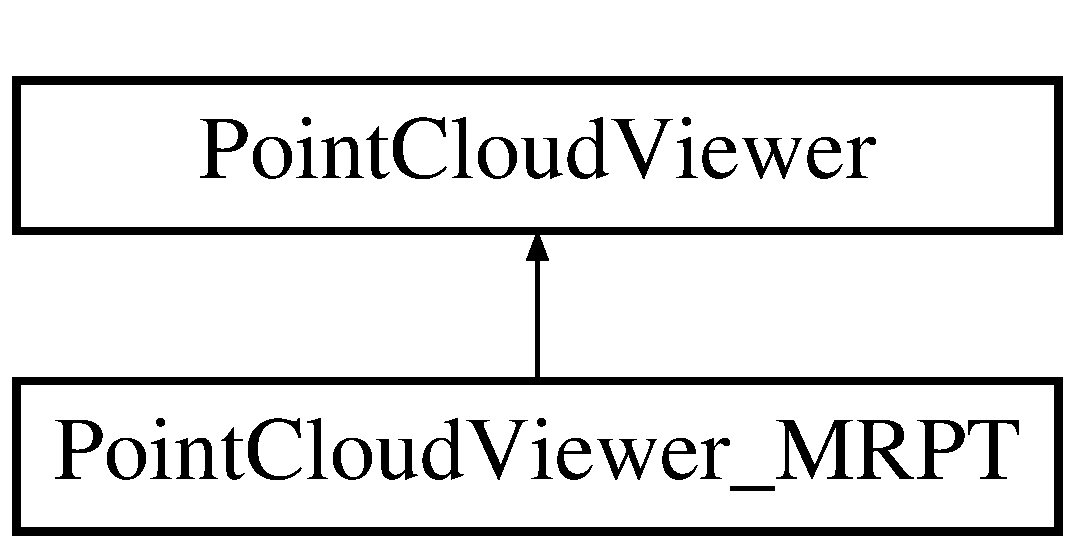
\includegraphics[height=2.000000cm]{class_point_cloud_viewer}
\end{center}
\end{figure}
\subsection*{Public Member Functions}
\begin{DoxyCompactItemize}
\item 
\hypertarget{class_point_cloud_viewer_a815f222fe31422c9230a1ecb1c306f15}{
virtual void {\bfseries showPointCloud} (pcl::PointCloud$<$ pcl::PointXYZRGB $>$ \&)=0}
\label{class_point_cloud_viewer_a815f222fe31422c9230a1ecb1c306f15}

\item 
\hypertarget{class_point_cloud_viewer_a10f36af1f2c77cdc68911c0b76fb1125}{
virtual bool {\bfseries isOpen} ()=0}
\label{class_point_cloud_viewer_a10f36af1f2c77cdc68911c0b76fb1125}

\end{DoxyCompactItemize}


\subsection{Detailed Description}
Abstract class \hyperlink{class_point_cloud_viewer}{PointCloudViewer} 

The documentation for this class was generated from the following file:\begin{DoxyCompactItemize}
\item 
PointCloudViewer.h\end{DoxyCompactItemize}

\hypertarget{class_point_cloud_viewer___m_r_p_t}{
\section{PointCloudViewer\_\-MRPT Class Reference}
\label{class_point_cloud_viewer___m_r_p_t}\index{PointCloudViewer\_\-MRPT@{PointCloudViewer\_\-MRPT}}
}
Inheritance diagram for PointCloudViewer\_\-MRPT:\begin{figure}[H]
\begin{center}
\leavevmode
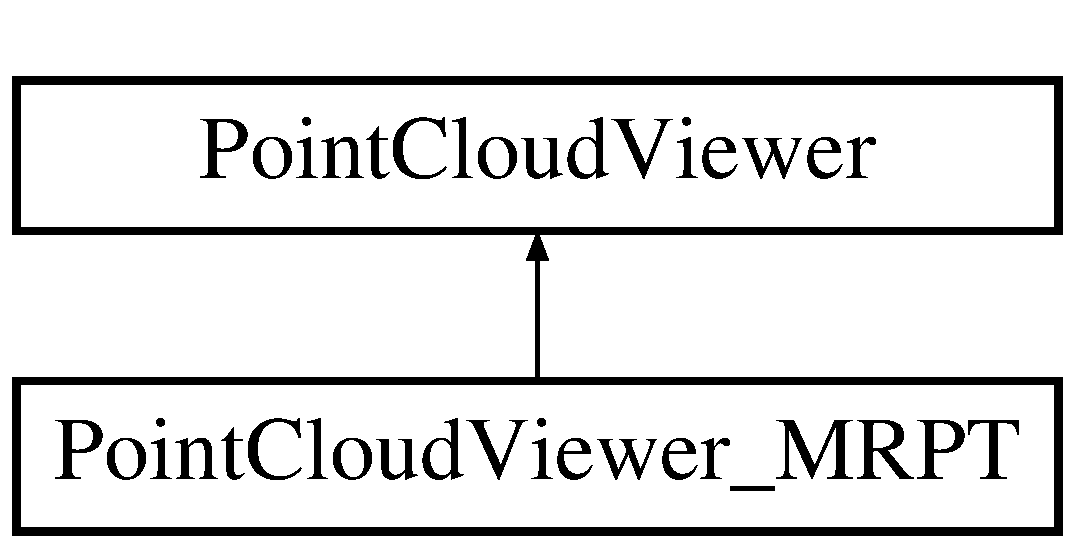
\includegraphics[height=2.000000cm]{class_point_cloud_viewer___m_r_p_t}
\end{center}
\end{figure}
\subsection*{Public Member Functions}
\begin{DoxyCompactItemize}
\item 
\hypertarget{class_point_cloud_viewer___m_r_p_t_a8c804b0f876740a8c1ad816250eb1bde}{
{\bfseries PointCloudViewer\_\-MRPT} (const std::string \&)}
\label{class_point_cloud_viewer___m_r_p_t_a8c804b0f876740a8c1ad816250eb1bde}

\item 
\hypertarget{class_point_cloud_viewer___m_r_p_t_a0d075bd0649fece16c544ff29ab8bfea}{
void {\bfseries showPointCloud} (pcl::PointCloud$<$ pcl::PointXYZRGB $>$ \&)}
\label{class_point_cloud_viewer___m_r_p_t_a0d075bd0649fece16c544ff29ab8bfea}

\item 
\hypertarget{class_point_cloud_viewer___m_r_p_t_ae531a413cdb4ed13e0e68d380dec6bad}{
bool {\bfseries isOpen} ()}
\label{class_point_cloud_viewer___m_r_p_t_ae531a413cdb4ed13e0e68d380dec6bad}

\end{DoxyCompactItemize}
\subsection*{Private Attributes}
\begin{DoxyCompactItemize}
\item 
\hypertarget{class_point_cloud_viewer___m_r_p_t_a63ec254507d94ddbf015f971f9eb3394}{
mrpt::gui::CDisplayWindow3D {\bfseries win3D}}
\label{class_point_cloud_viewer___m_r_p_t_a63ec254507d94ddbf015f971f9eb3394}

\item 
\hypertarget{class_point_cloud_viewer___m_r_p_t_a283adbfa64f409aaa12e0722e94accc4}{
mrpt::opengl::CPointCloudColouredPtr {\bfseries gl\_\-points}}
\label{class_point_cloud_viewer___m_r_p_t_a283adbfa64f409aaa12e0722e94accc4}

\item 
\hypertarget{class_point_cloud_viewer___m_r_p_t_a8a6762489cce8534892b073aa957a371}{
mrpt::opengl::COpenGLViewportPtr {\bfseries viewInt}}
\label{class_point_cloud_viewer___m_r_p_t_a8a6762489cce8534892b073aa957a371}

\item 
\hypertarget{class_point_cloud_viewer___m_r_p_t_a34c427f74ea251956fa06735add96034}{
bool {\bfseries escPressed}}
\label{class_point_cloud_viewer___m_r_p_t_a34c427f74ea251956fa06735add96034}

\end{DoxyCompactItemize}


The documentation for this class was generated from the following file:\begin{DoxyCompactItemize}
\item 
PointCloudViewer\_\-MRPT.h\end{DoxyCompactItemize}

\hypertarget{struct_kinect_grabber___m_r_p_t_1_1_t_thread_param}{
\section{KinectGrabber\_\-MRPT::TThreadParam Struct Reference}
\label{struct_kinect_grabber___m_r_p_t_1_1_t_thread_param}\index{KinectGrabber\_\-MRPT::TThreadParam@{KinectGrabber\_\-MRPT::TThreadParam}}
}
\subsection*{Data Fields}
\begin{DoxyCompactItemize}
\item 
\hypertarget{struct_kinect_grabber___m_r_p_t_1_1_t_thread_param_a498162673751ccf387f5c9ddcf4d9812}{
volatile bool {\bfseries quit}}
\label{struct_kinect_grabber___m_r_p_t_1_1_t_thread_param_a498162673751ccf387f5c9ddcf4d9812}

\item 
\hypertarget{struct_kinect_grabber___m_r_p_t_1_1_t_thread_param_a9ef42273f5f6ac0e1b8741d7b9875a38}{
volatile int {\bfseries pushed\_\-key}}
\label{struct_kinect_grabber___m_r_p_t_1_1_t_thread_param_a9ef42273f5f6ac0e1b8741d7b9875a38}

\item 
\hypertarget{struct_kinect_grabber___m_r_p_t_1_1_t_thread_param_a30eb58aadbfa1a861955776e37e6b509}{
volatile double {\bfseries tilt\_\-ang\_\-deg}}
\label{struct_kinect_grabber___m_r_p_t_1_1_t_thread_param_a30eb58aadbfa1a861955776e37e6b509}

\item 
\hypertarget{struct_kinect_grabber___m_r_p_t_1_1_t_thread_param_a0a01691754dd95a575b7eaa614a33498}{
volatile double {\bfseries Hz}}
\label{struct_kinect_grabber___m_r_p_t_1_1_t_thread_param_a0a01691754dd95a575b7eaa614a33498}

\item 
\hypertarget{struct_kinect_grabber___m_r_p_t_1_1_t_thread_param_abb407ff1abba227249f6efea5adc78aa}{
mrpt::synch::CThreadSafeVariable$<$ CObservation3DRangeScanPtr $>$ {\bfseries new\_\-obs}}
\label{struct_kinect_grabber___m_r_p_t_1_1_t_thread_param_abb407ff1abba227249f6efea5adc78aa}

\item 
\hypertarget{struct_kinect_grabber___m_r_p_t_1_1_t_thread_param_a020c5c2516b0731ba2f7604642bcba65}{
mrpt::synch::CThreadSafeVariable$<$ CObservationIMUPtr $>$ {\bfseries new\_\-obs\_\-imu}}
\label{struct_kinect_grabber___m_r_p_t_1_1_t_thread_param_a020c5c2516b0731ba2f7604642bcba65}

\end{DoxyCompactItemize}


The documentation for this struct was generated from the following file:\begin{DoxyCompactItemize}
\item 
KinectGrabber\_\-MRPT.h\end{DoxyCompactItemize}

\hypertarget{struct_kinect_grabber___rawlog_1_1_t_thread_param}{
\section{KinectGrabber\_\-Rawlog::TThreadParam Struct Reference}
\label{struct_kinect_grabber___rawlog_1_1_t_thread_param}\index{KinectGrabber\_\-Rawlog::TThreadParam@{KinectGrabber\_\-Rawlog::TThreadParam}}
}
\subsection*{Public Member Functions}
\begin{DoxyCompactItemize}
\item 
\hypertarget{struct_kinect_grabber___rawlog_1_1_t_thread_param_ad74f52ed635f96eccd143d0d82975342}{
{\bfseries TThreadParam} (const std::string \&\_\-rawlog\_\-file=std::string(), bool \_\-generate\_\-3D\_\-pointcloud\_\-in\_\-this\_\-thread=false)}
\label{struct_kinect_grabber___rawlog_1_1_t_thread_param_ad74f52ed635f96eccd143d0d82975342}

\end{DoxyCompactItemize}
\subsection*{Data Fields}
\begin{DoxyCompactItemize}
\item 
\hypertarget{struct_kinect_grabber___rawlog_1_1_t_thread_param_a8e14ab7dafc94eb16a4db364fd6a0c37}{
const std::string \hyperlink{struct_kinect_grabber___rawlog_1_1_t_thread_param_a8e14ab7dafc94eb16a4db364fd6a0c37}{rawlog\_\-file}}
\label{struct_kinect_grabber___rawlog_1_1_t_thread_param_a8e14ab7dafc94eb16a4db364fd6a0c37}

\begin{DoxyCompactList}\small\item\em Only when is\_\-online==false. \item\end{DoxyCompactList}\item 
\hypertarget{struct_kinect_grabber___rawlog_1_1_t_thread_param_a4647b7cc25bc1963cc0d175de116f30f}{
const bool \hyperlink{struct_kinect_grabber___rawlog_1_1_t_thread_param_a4647b7cc25bc1963cc0d175de116f30f}{generate\_\-3D\_\-pointcloud\_\-in\_\-this\_\-thread}}
\label{struct_kinect_grabber___rawlog_1_1_t_thread_param_a4647b7cc25bc1963cc0d175de116f30f}

\begin{DoxyCompactList}\small\item\em true: populate the 3D point fields in the output observation; false: only RGB and Depth images. \item\end{DoxyCompactList}\item 
\hypertarget{struct_kinect_grabber___rawlog_1_1_t_thread_param_a32ec19b416203aebb2993d6466a86a15}{
volatile bool \hyperlink{struct_kinect_grabber___rawlog_1_1_t_thread_param_a32ec19b416203aebb2993d6466a86a15}{quit}}
\label{struct_kinect_grabber___rawlog_1_1_t_thread_param_a32ec19b416203aebb2993d6466a86a15}

\begin{DoxyCompactList}\small\item\em In/Out variable: Forces the thread to exit or indicates an error in the thread that caused it to end. \item\end{DoxyCompactList}\item 
\hypertarget{struct_kinect_grabber___rawlog_1_1_t_thread_param_aac0203113ffaad5599395431050ac37a}{
volatile double \hyperlink{struct_kinect_grabber___rawlog_1_1_t_thread_param_aac0203113ffaad5599395431050ac37a}{Hz}}
\label{struct_kinect_grabber___rawlog_1_1_t_thread_param_aac0203113ffaad5599395431050ac37a}

\begin{DoxyCompactList}\small\item\em Out variable: Approx. capturing rate from the thread. \item\end{DoxyCompactList}\item 
\hypertarget{struct_kinect_grabber___rawlog_1_1_t_thread_param_a8cf656cbaab31b17e8794674706efa50}{
mrpt::synch::CThreadSafeVariable$<$ mrpt::slam::CObservation3DRangeScanPtr $>$ \hyperlink{struct_kinect_grabber___rawlog_1_1_t_thread_param_a8cf656cbaab31b17e8794674706efa50}{new\_\-obs}}
\label{struct_kinect_grabber___rawlog_1_1_t_thread_param_a8cf656cbaab31b17e8794674706efa50}

\begin{DoxyCompactList}\small\item\em RGB+D (+ optionally, 3D point cloud) \item\end{DoxyCompactList}\end{DoxyCompactItemize}


The documentation for this struct was generated from the following file:\begin{DoxyCompactItemize}
\item 
KinectGrabber\_\-Rawlog.h\end{DoxyCompactItemize}

\hypertarget{class_visual3_d_rigid_transformation_estimator}{
\section{Visual3DRigidTransformationEstimator Class Reference}
\label{class_visual3_d_rigid_transformation_estimator}\index{Visual3DRigidTransformationEstimator@{Visual3DRigidTransformationEstimator}}
}


{\ttfamily \#include $<$Visual3DRigidTransformationEstimator.h$>$}

Inheritance diagram for Visual3DRigidTransformationEstimator:\begin{figure}[H]
\begin{center}
\leavevmode
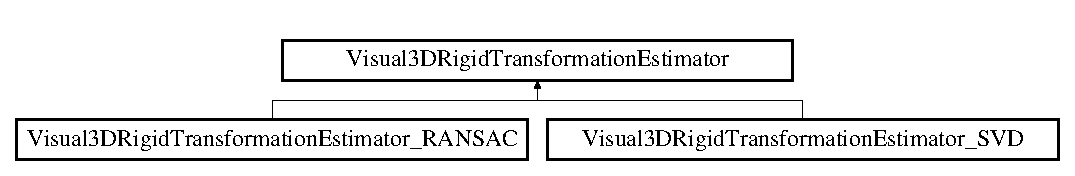
\includegraphics[height=1.911263cm]{class_visual3_d_rigid_transformation_estimator}
\end{center}
\end{figure}
\subsection*{Public Member Functions}
\begin{DoxyCompactItemize}
\item 
virtual int \hyperlink{class_visual3_d_rigid_transformation_estimator_a2f431dce774df16f4950840ec1d1f37c}{estimateVisual3DRigidTransformation} (const std::vector$<$ cv::Point2f $>$ \&points1, const std::vector$<$ cv::Point2f $>$ \&points2, const pcl::PointCloud$<$ pcl::PointXYZRGB $>$::Ptr \&pointCloudPtr1, const pcl::PointCloud$<$ pcl::PointXYZRGB $>$::Ptr \&pointCloudPtr2, Eigen::Matrix4f \&rigidTransformation)=0
\end{DoxyCompactItemize}


\subsection{Detailed Description}
Abstract class that specifies a method to estimate the 3D rigid transformation that best align a pair of 3D correspondences of two given point clouds. 

\subsection{Member Function Documentation}
\hypertarget{class_visual3_d_rigid_transformation_estimator_a2f431dce774df16f4950840ec1d1f37c}{
\index{Visual3DRigidTransformationEstimator@{Visual3DRigidTransformationEstimator}!estimateVisual3DRigidTransformation@{estimateVisual3DRigidTransformation}}
\index{estimateVisual3DRigidTransformation@{estimateVisual3DRigidTransformation}!Visual3DRigidTransformationEstimator@{Visual3DRigidTransformationEstimator}}
\subsubsection[{estimateVisual3DRigidTransformation}]{\setlength{\rightskip}{0pt plus 5cm}virtual int Visual3DRigidTransformationEstimator::estimateVisual3DRigidTransformation (
\begin{DoxyParamCaption}
\item[{const std::vector$<$ cv::Point2f $>$ \&}]{points1, }
\item[{const std::vector$<$ cv::Point2f $>$ \&}]{points2, }
\item[{const pcl::PointCloud$<$ pcl::PointXYZRGB $>$::Ptr \&}]{pointCloudPtr1, }
\item[{const pcl::PointCloud$<$ pcl::PointXYZRGB $>$::Ptr \&}]{pointCloudPtr2, }
\item[{Eigen::Matrix4f \&}]{rigidTransformation}
\end{DoxyParamCaption}
)\hspace{0.3cm}{\ttfamily  \mbox{[}pure virtual\mbox{]}}}}
\label{class_visual3_d_rigid_transformation_estimator_a2f431dce774df16f4950840ec1d1f37c}
Estimates the 3D rigid transformation that best align a pair of 3D point correspondences of two given point clouds. The method takes two vectors of 2D points that determines the pairs of correspondences and two 3D point clouds. The algorithm then takes the 3D points corresponding to the 2D correspondences to estimate the 3D rigid transformation. 

Implemented in \hyperlink{class_visual3_d_rigid_transformation_estimator___r_a_n_s_a_c_a1e97ade711022e984566bbed9561a46a}{Visual3DRigidTransformationEstimator\_\-RANSAC}, and \hyperlink{class_visual3_d_rigid_transformation_estimator___s_v_d_a6033ab7c16772b318d7c951474f42047}{Visual3DRigidTransformationEstimator\_\-SVD}.



The documentation for this class was generated from the following file:\begin{DoxyCompactItemize}
\item 
Visual3DRigidTransformationEstimator.h\end{DoxyCompactItemize}

\hypertarget{class_visual3_d_rigid_transformation_estimator___r_a_n_s_a_c}{
\section{Visual3DRigidTransformationEstimator\_\-RANSAC Class Reference}
\label{class_visual3_d_rigid_transformation_estimator___r_a_n_s_a_c}\index{Visual3DRigidTransformationEstimator\_\-RANSAC@{Visual3DRigidTransformationEstimator\_\-RANSAC}}
}


{\ttfamily \#include $<$Visual3DRigidTransformationEstimator\_\-RANSAC.h$>$}

Inheritance diagram for Visual3DRigidTransformationEstimator\_\-RANSAC:\begin{figure}[H]
\begin{center}
\leavevmode
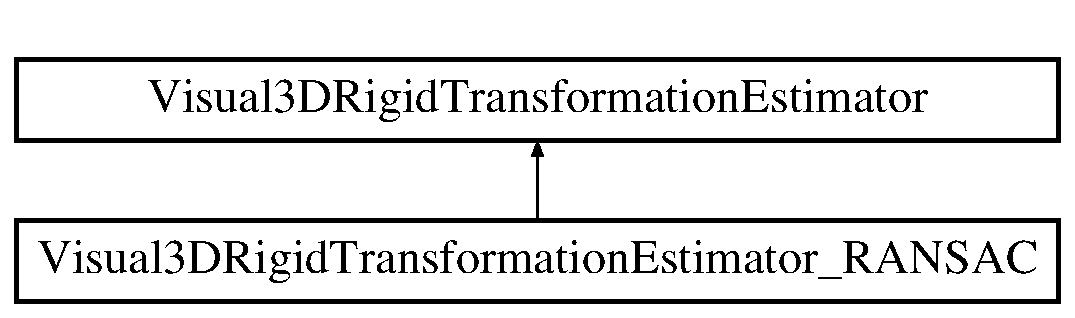
\includegraphics[height=2.000000cm]{class_visual3_d_rigid_transformation_estimator___r_a_n_s_a_c}
\end{center}
\end{figure}
\subsection*{Public Member Functions}
\begin{DoxyCompactItemize}
\item 
\hyperlink{class_visual3_d_rigid_transformation_estimator___r_a_n_s_a_c_a73fc605acb5765ffe6bef88b3c025625}{Visual3DRigidTransformationEstimator\_\-RANSAC} (const double=0.05, const double=10.0)
\item 
void \hyperlink{class_visual3_d_rigid_transformation_estimator___r_a_n_s_a_c_adc981ee0d2fc15c0c5273cfbc7a353b0}{setMinDepthValue} (const double)
\item 
void \hyperlink{class_visual3_d_rigid_transformation_estimator___r_a_n_s_a_c_af74500de40c35f98785de01a3baf5143}{setMaxDepthValue} (const double)
\item 
int \hyperlink{class_visual3_d_rigid_transformation_estimator___r_a_n_s_a_c_a1e97ade711022e984566bbed9561a46a}{estimateVisual3DRigidTransformation} (const std::vector$<$ cv::Point2f $>$ \&points1, const std::vector$<$ cv::Point2f $>$ \&points2, const pcl::PointCloud$<$ pcl::PointXYZRGB $>$::Ptr \&pointCloudPtr1, const pcl::PointCloud$<$ pcl::PointXYZRGB $>$::Ptr \&pointCloudPtr2, Eigen::Matrix4f \&rigidTransformation)
\end{DoxyCompactItemize}
\subsection*{Private Member Functions}
\begin{DoxyCompactItemize}
\item 
\hypertarget{class_visual3_d_rigid_transformation_estimator___r_a_n_s_a_c_aaee81e09d6622e1a5a69f9f1c341884a}{
void {\bfseries matchesWith3DValidData} (const std::vector$<$ cv::Point2f $>$ \&, const std::vector$<$ cv::Point2f $>$ \&, const pcl::PointCloud$<$ pcl::PointXYZRGB $>$::Ptr \&, const pcl::PointCloud$<$ pcl::PointXYZRGB $>$::Ptr \&)}
\label{class_visual3_d_rigid_transformation_estimator___r_a_n_s_a_c_aaee81e09d6622e1a5a69f9f1c341884a}

\end{DoxyCompactItemize}
\subsection*{Private Attributes}
\begin{DoxyCompactItemize}
\item 
\hypertarget{class_visual3_d_rigid_transformation_estimator___r_a_n_s_a_c_a213b24bc3de5c061791cedd48e5343fa}{
pcl::registration::CorrespondenceRejectorSampleConsensus$<$ pcl::PointXYZRGB $>$ {\bfseries corrsRejectorSAC}}
\label{class_visual3_d_rigid_transformation_estimator___r_a_n_s_a_c_a213b24bc3de5c061791cedd48e5343fa}

\item 
\hypertarget{class_visual3_d_rigid_transformation_estimator___r_a_n_s_a_c_aac560055af9973e994c79debbc39ae72}{
boost::shared\_\-ptr$<$ pcl::Correspondences $>$ {\bfseries correspondences}}
\label{class_visual3_d_rigid_transformation_estimator___r_a_n_s_a_c_aac560055af9973e994c79debbc39ae72}

\item 
\hypertarget{class_visual3_d_rigid_transformation_estimator___r_a_n_s_a_c_aed18e1b68f2b6cf19fc81af88b6fbe63}{
double {\bfseries minDepthValue}}
\label{class_visual3_d_rigid_transformation_estimator___r_a_n_s_a_c_aed18e1b68f2b6cf19fc81af88b6fbe63}

\item 
\hypertarget{class_visual3_d_rigid_transformation_estimator___r_a_n_s_a_c_afae1bb594a06159e76b9808d7d329655}{
double {\bfseries maxDepthValue}}
\label{class_visual3_d_rigid_transformation_estimator___r_a_n_s_a_c_afae1bb594a06159e76b9808d7d329655}

\end{DoxyCompactItemize}


\subsection{Detailed Description}
This class encapsulates the functionality of a 3D rigid transformation estimator to compute a rigid transformation robust to incorrect correspondences (RANSAC) using the PCL registration module. 

\subsection{Constructor \& Destructor Documentation}
\hypertarget{class_visual3_d_rigid_transformation_estimator___r_a_n_s_a_c_a73fc605acb5765ffe6bef88b3c025625}{
\index{Visual3DRigidTransformationEstimator\_\-RANSAC@{Visual3DRigidTransformationEstimator\_\-RANSAC}!Visual3DRigidTransformationEstimator\_\-RANSAC@{Visual3DRigidTransformationEstimator\_\-RANSAC}}
\index{Visual3DRigidTransformationEstimator\_\-RANSAC@{Visual3DRigidTransformationEstimator\_\-RANSAC}!Visual3DRigidTransformationEstimator_RANSAC@{Visual3DRigidTransformationEstimator\_\-RANSAC}}
\subsubsection[{Visual3DRigidTransformationEstimator\_\-RANSAC}]{\setlength{\rightskip}{0pt plus 5cm}Visual3DRigidTransformationEstimator\_\-RANSAC::Visual3DRigidTransformationEstimator\_\-RANSAC (
\begin{DoxyParamCaption}
\item[{const double}]{ = {\ttfamily 0.05}, }
\item[{const double}]{ = {\ttfamily 10.0}}
\end{DoxyParamCaption}
)}}
\label{class_visual3_d_rigid_transformation_estimator___r_a_n_s_a_c_a73fc605acb5765ffe6bef88b3c025625}
Constructor of an instance of \hyperlink{class_visual3_d_rigid_transformation_estimator___r_a_n_s_a_c}{Visual3DRigidTransformationEstimator\_\-RANSAC} with a given minDepthValue and maxDepthValue that specifies a valid range of 3D points (in meters). 

\subsection{Member Function Documentation}
\hypertarget{class_visual3_d_rigid_transformation_estimator___r_a_n_s_a_c_a1e97ade711022e984566bbed9561a46a}{
\index{Visual3DRigidTransformationEstimator\_\-RANSAC@{Visual3DRigidTransformationEstimator\_\-RANSAC}!estimateVisual3DRigidTransformation@{estimateVisual3DRigidTransformation}}
\index{estimateVisual3DRigidTransformation@{estimateVisual3DRigidTransformation}!Visual3DRigidTransformationEstimator_RANSAC@{Visual3DRigidTransformationEstimator\_\-RANSAC}}
\subsubsection[{estimateVisual3DRigidTransformation}]{\setlength{\rightskip}{0pt plus 5cm}int Visual3DRigidTransformationEstimator\_\-RANSAC::estimateVisual3DRigidTransformation (
\begin{DoxyParamCaption}
\item[{const std::vector$<$ cv::Point2f $>$ \&}]{points1, }
\item[{const std::vector$<$ cv::Point2f $>$ \&}]{points2, }
\item[{const pcl::PointCloud$<$ pcl::PointXYZRGB $>$::Ptr \&}]{pointCloudPtr1, }
\item[{const pcl::PointCloud$<$ pcl::PointXYZRGB $>$::Ptr \&}]{pointCloudPtr2, }
\item[{Eigen::Matrix4f \&}]{rigidTransformation}
\end{DoxyParamCaption}
)\hspace{0.3cm}{\ttfamily  \mbox{[}virtual\mbox{]}}}}
\label{class_visual3_d_rigid_transformation_estimator___r_a_n_s_a_c_a1e97ade711022e984566bbed9561a46a}
Estimates the 3D rigid transformation that best align a pair of 3D point correspondences of two given point clouds. The method takes two vectors of 2D points that determines the pairs of correspondences and two 3D point clouds. The algorithm then takes the 3D points corresponding to the 2D correspondences to estimate the 3D rigid transformation. The algorithm uses RANSAC to make the method robust to outliers. 

Implements \hyperlink{class_visual3_d_rigid_transformation_estimator_a2f431dce774df16f4950840ec1d1f37c}{Visual3DRigidTransformationEstimator}.

\hypertarget{class_visual3_d_rigid_transformation_estimator___r_a_n_s_a_c_af74500de40c35f98785de01a3baf5143}{
\index{Visual3DRigidTransformationEstimator\_\-RANSAC@{Visual3DRigidTransformationEstimator\_\-RANSAC}!setMaxDepthValue@{setMaxDepthValue}}
\index{setMaxDepthValue@{setMaxDepthValue}!Visual3DRigidTransformationEstimator_RANSAC@{Visual3DRigidTransformationEstimator\_\-RANSAC}}
\subsubsection[{setMaxDepthValue}]{\setlength{\rightskip}{0pt plus 5cm}void Visual3DRigidTransformationEstimator\_\-RANSAC::setMaxDepthValue (
\begin{DoxyParamCaption}
\item[{const double}]{}
\end{DoxyParamCaption}
)}}
\label{class_visual3_d_rigid_transformation_estimator___r_a_n_s_a_c_af74500de40c35f98785de01a3baf5143}
Sets the maxDepthValue to the specified value (in meters) \hypertarget{class_visual3_d_rigid_transformation_estimator___r_a_n_s_a_c_adc981ee0d2fc15c0c5273cfbc7a353b0}{
\index{Visual3DRigidTransformationEstimator\_\-RANSAC@{Visual3DRigidTransformationEstimator\_\-RANSAC}!setMinDepthValue@{setMinDepthValue}}
\index{setMinDepthValue@{setMinDepthValue}!Visual3DRigidTransformationEstimator_RANSAC@{Visual3DRigidTransformationEstimator\_\-RANSAC}}
\subsubsection[{setMinDepthValue}]{\setlength{\rightskip}{0pt plus 5cm}void Visual3DRigidTransformationEstimator\_\-RANSAC::setMinDepthValue (
\begin{DoxyParamCaption}
\item[{const double}]{}
\end{DoxyParamCaption}
)}}
\label{class_visual3_d_rigid_transformation_estimator___r_a_n_s_a_c_adc981ee0d2fc15c0c5273cfbc7a353b0}
Sets the minDepthValue to the specified value (in meters) 

The documentation for this class was generated from the following file:\begin{DoxyCompactItemize}
\item 
Visual3DRigidTransformationEstimator\_\-RANSAC.h\end{DoxyCompactItemize}

\hypertarget{class_visual3_d_rigid_transformation_estimator___s_v_d}{
\section{Visual3DRigidTransformationEstimator\_\-SVD Class Reference}
\label{class_visual3_d_rigid_transformation_estimator___s_v_d}\index{Visual3DRigidTransformationEstimator\_\-SVD@{Visual3DRigidTransformationEstimator\_\-SVD}}
}


{\ttfamily \#include $<$Visual3DRigidTransformationEstimator\_\-SVD.h$>$}

Inheritance diagram for Visual3DRigidTransformationEstimator\_\-SVD:\begin{figure}[H]
\begin{center}
\leavevmode
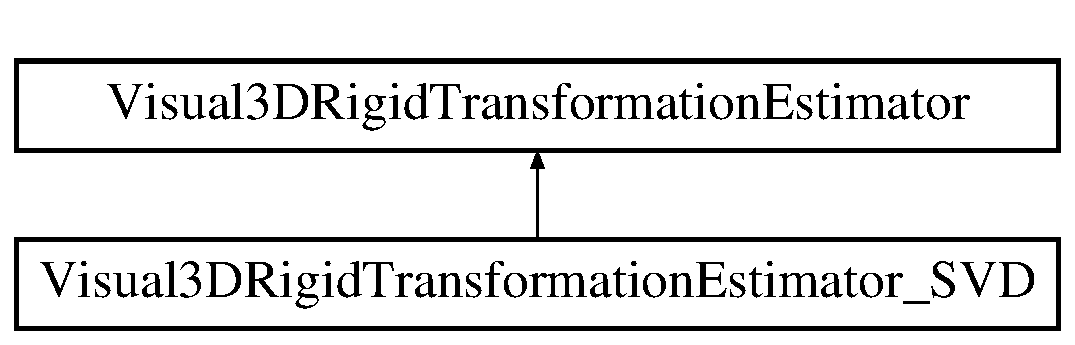
\includegraphics[height=2.000000cm]{class_visual3_d_rigid_transformation_estimator___s_v_d}
\end{center}
\end{figure}
\subsection*{Public Member Functions}
\begin{DoxyCompactItemize}
\item 
\hyperlink{class_visual3_d_rigid_transformation_estimator___s_v_d_ac5a8b46d9f825bd77a68ae9218e480bb}{Visual3DRigidTransformationEstimator\_\-SVD} (const double=0.05, const double=10.0)
\item 
void \hyperlink{class_visual3_d_rigid_transformation_estimator___s_v_d_a14b1d5d2222d41ac059f4f567fb41339}{setMinDepthValue} (const double)
\item 
void \hyperlink{class_visual3_d_rigid_transformation_estimator___s_v_d_a5d94cd8297bc8ea6eefe4cf996153294}{setMaxDepthValue} (const double)
\item 
int \hyperlink{class_visual3_d_rigid_transformation_estimator___s_v_d_a6033ab7c16772b318d7c951474f42047}{estimateVisual3DRigidTransformation} (const std::vector$<$ cv::Point2f $>$ \&points1, const std::vector$<$ cv::Point2f $>$ \&points2, const pcl::PointCloud$<$ pcl::PointXYZRGB $>$::Ptr \&pointCloudPtr1, const pcl::PointCloud$<$ pcl::PointXYZRGB $>$::Ptr \&pointCloudPtr2, Eigen::Matrix4f \&rigidTransformation)
\end{DoxyCompactItemize}
\subsection*{Private Member Functions}
\begin{DoxyCompactItemize}
\item 
\hypertarget{class_visual3_d_rigid_transformation_estimator___s_v_d_af1fa6a350cc3c2474eba5b1378408456}{
void {\bfseries matchesWith3DValidData} (const std::vector$<$ cv::Point2f $>$ \&, const std::vector$<$ cv::Point2f $>$ \&, const pcl::PointCloud$<$ pcl::PointXYZRGB $>$::Ptr \&, const pcl::PointCloud$<$ pcl::PointXYZRGB $>$::Ptr \&)}
\label{class_visual3_d_rigid_transformation_estimator___s_v_d_af1fa6a350cc3c2474eba5b1378408456}

\end{DoxyCompactItemize}
\subsection*{Private Attributes}
\begin{DoxyCompactItemize}
\item 
\hypertarget{class_visual3_d_rigid_transformation_estimator___s_v_d_a24d05019fb93f19d200eb4cc8cfafc26}{
pcl::registration::TransformationEstimationSVD$<$ pcl::PointXYZRGB, pcl::PointXYZRGB $>$ {\bfseries transformationEstimator}}
\label{class_visual3_d_rigid_transformation_estimator___s_v_d_a24d05019fb93f19d200eb4cc8cfafc26}

\item 
\hypertarget{class_visual3_d_rigid_transformation_estimator___s_v_d_ae299454fce2ae52c5ea0a9f81e8a55a5}{
pcl::Correspondences {\bfseries correspondences}}
\label{class_visual3_d_rigid_transformation_estimator___s_v_d_ae299454fce2ae52c5ea0a9f81e8a55a5}

\item 
\hypertarget{class_visual3_d_rigid_transformation_estimator___s_v_d_a90621e4cc84c2d8251db3922f1c44582}{
double {\bfseries minDepthValue}}
\label{class_visual3_d_rigid_transformation_estimator___s_v_d_a90621e4cc84c2d8251db3922f1c44582}

\item 
\hypertarget{class_visual3_d_rigid_transformation_estimator___s_v_d_a08f88e98013c9eaad11c289fe45ceaa8}{
double {\bfseries maxDepthValue}}
\label{class_visual3_d_rigid_transformation_estimator___s_v_d_a08f88e98013c9eaad11c289fe45ceaa8}

\end{DoxyCompactItemize}


\subsection{Detailed Description}
This class encapsulates the functionality of a 3D rigid transformation estimator to compute a rigid transformation using the SVD algorithm. This implementation considers that there isn't incorrect correspondences and could produce incorrect rigid transformations in presence of outliers. 

\subsection{Constructor \& Destructor Documentation}
\hypertarget{class_visual3_d_rigid_transformation_estimator___s_v_d_ac5a8b46d9f825bd77a68ae9218e480bb}{
\index{Visual3DRigidTransformationEstimator\_\-SVD@{Visual3DRigidTransformationEstimator\_\-SVD}!Visual3DRigidTransformationEstimator\_\-SVD@{Visual3DRigidTransformationEstimator\_\-SVD}}
\index{Visual3DRigidTransformationEstimator\_\-SVD@{Visual3DRigidTransformationEstimator\_\-SVD}!Visual3DRigidTransformationEstimator_SVD@{Visual3DRigidTransformationEstimator\_\-SVD}}
\subsubsection[{Visual3DRigidTransformationEstimator\_\-SVD}]{\setlength{\rightskip}{0pt plus 5cm}Visual3DRigidTransformationEstimator\_\-SVD::Visual3DRigidTransformationEstimator\_\-SVD (
\begin{DoxyParamCaption}
\item[{const double}]{ = {\ttfamily 0.05}, }
\item[{const double}]{ = {\ttfamily 10.0}}
\end{DoxyParamCaption}
)}}
\label{class_visual3_d_rigid_transformation_estimator___s_v_d_ac5a8b46d9f825bd77a68ae9218e480bb}
Constructor of an instance of \hyperlink{class_visual3_d_rigid_transformation_estimator___s_v_d}{Visual3DRigidTransformationEstimator\_\-SVD} with a given minDepthValue and maxDepthValue that specifies a valid range of 3D points (in meters). 

\subsection{Member Function Documentation}
\hypertarget{class_visual3_d_rigid_transformation_estimator___s_v_d_a6033ab7c16772b318d7c951474f42047}{
\index{Visual3DRigidTransformationEstimator\_\-SVD@{Visual3DRigidTransformationEstimator\_\-SVD}!estimateVisual3DRigidTransformation@{estimateVisual3DRigidTransformation}}
\index{estimateVisual3DRigidTransformation@{estimateVisual3DRigidTransformation}!Visual3DRigidTransformationEstimator_SVD@{Visual3DRigidTransformationEstimator\_\-SVD}}
\subsubsection[{estimateVisual3DRigidTransformation}]{\setlength{\rightskip}{0pt plus 5cm}int Visual3DRigidTransformationEstimator\_\-SVD::estimateVisual3DRigidTransformation (
\begin{DoxyParamCaption}
\item[{const std::vector$<$ cv::Point2f $>$ \&}]{points1, }
\item[{const std::vector$<$ cv::Point2f $>$ \&}]{points2, }
\item[{const pcl::PointCloud$<$ pcl::PointXYZRGB $>$::Ptr \&}]{pointCloudPtr1, }
\item[{const pcl::PointCloud$<$ pcl::PointXYZRGB $>$::Ptr \&}]{pointCloudPtr2, }
\item[{Eigen::Matrix4f \&}]{rigidTransformation}
\end{DoxyParamCaption}
)\hspace{0.3cm}{\ttfamily  \mbox{[}virtual\mbox{]}}}}
\label{class_visual3_d_rigid_transformation_estimator___s_v_d_a6033ab7c16772b318d7c951474f42047}
Estimates the 3D rigid transformation that best align a pair of 3D point correspondences of two given point clouds. The method takes two vectors of 2D points that determines the pairs of correspondences and two 3D point clouds. The algorithm then takes the 3D points corresponding to the 2D correspondences to estimate the 3D rigid transformation. This method should not be used in presence of outliers. In that case use the robustified method encapsulated in the class \hyperlink{class_visual3_d_rigid_transformation_estimator___r_a_n_s_a_c}{Visual3DRigidTransformationEstimator\_\-RANSAC}. 

Implements \hyperlink{class_visual3_d_rigid_transformation_estimator_a2f431dce774df16f4950840ec1d1f37c}{Visual3DRigidTransformationEstimator}.

\hypertarget{class_visual3_d_rigid_transformation_estimator___s_v_d_a5d94cd8297bc8ea6eefe4cf996153294}{
\index{Visual3DRigidTransformationEstimator\_\-SVD@{Visual3DRigidTransformationEstimator\_\-SVD}!setMaxDepthValue@{setMaxDepthValue}}
\index{setMaxDepthValue@{setMaxDepthValue}!Visual3DRigidTransformationEstimator_SVD@{Visual3DRigidTransformationEstimator\_\-SVD}}
\subsubsection[{setMaxDepthValue}]{\setlength{\rightskip}{0pt plus 5cm}void Visual3DRigidTransformationEstimator\_\-SVD::setMaxDepthValue (
\begin{DoxyParamCaption}
\item[{const double}]{}
\end{DoxyParamCaption}
)}}
\label{class_visual3_d_rigid_transformation_estimator___s_v_d_a5d94cd8297bc8ea6eefe4cf996153294}
Sets the maxDepthValue to the specified value (in meters) \hypertarget{class_visual3_d_rigid_transformation_estimator___s_v_d_a14b1d5d2222d41ac059f4f567fb41339}{
\index{Visual3DRigidTransformationEstimator\_\-SVD@{Visual3DRigidTransformationEstimator\_\-SVD}!setMinDepthValue@{setMinDepthValue}}
\index{setMinDepthValue@{setMinDepthValue}!Visual3DRigidTransformationEstimator_SVD@{Visual3DRigidTransformationEstimator\_\-SVD}}
\subsubsection[{setMinDepthValue}]{\setlength{\rightskip}{0pt plus 5cm}void Visual3DRigidTransformationEstimator\_\-SVD::setMinDepthValue (
\begin{DoxyParamCaption}
\item[{const double}]{}
\end{DoxyParamCaption}
)}}
\label{class_visual3_d_rigid_transformation_estimator___s_v_d_a14b1d5d2222d41ac059f4f567fb41339}
Sets the minDepthValue to the specified value (in meters) 

The documentation for this class was generated from the following file:\begin{DoxyCompactItemize}
\item 
Visual3DRigidTransformationEstimator\_\-SVD.h\end{DoxyCompactItemize}

\hypertarget{class_visual_feature_descriptor_extractor}{
\section{VisualFeatureDescriptorExtractor Class Reference}
\label{class_visual_feature_descriptor_extractor}\index{VisualFeatureDescriptorExtractor@{VisualFeatureDescriptorExtractor}}
}


{\ttfamily \#include $<$VisualFeatureDescriptorExtractor.h$>$}

Inheritance diagram for VisualFeatureDescriptorExtractor:\begin{figure}[H]
\begin{center}
\leavevmode
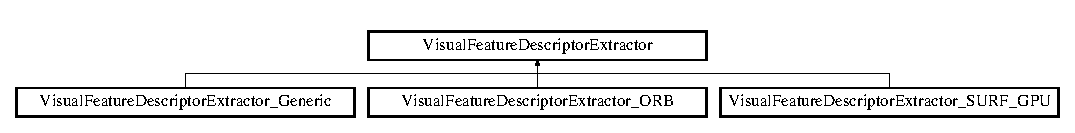
\includegraphics[height=1.333333cm]{class_visual_feature_descriptor_extractor}
\end{center}
\end{figure}
\subsection*{Public Member Functions}
\begin{DoxyCompactItemize}
\item 
virtual void \hyperlink{class_visual_feature_descriptor_extractor_a7852b85032fb28acdc73295dbda973ff}{setInputImage} (const cv::Mat \&image)
\item 
virtual void \hyperlink{class_visual_feature_descriptor_extractor_aac4d313540ff83e03fb5b0a0952fc0f4}{detectKeypointsAndComputeDescriptors} (std::vector$<$ cv::KeyPoint $>$ \&keypoints, cv::Mat \&descriptors, std::vector$<$ float $>$ \&descriptors\_\-aux)=0
\end{DoxyCompactItemize}
\subsection*{Protected Attributes}
\begin{DoxyCompactItemize}
\item 
\hypertarget{class_visual_feature_descriptor_extractor_a1238e32b54e5a0dcbd19f89f2d4becf7}{
cv::Mat {\bfseries inputImage}}
\label{class_visual_feature_descriptor_extractor_a1238e32b54e5a0dcbd19f89f2d4becf7}

\end{DoxyCompactItemize}


\subsection{Detailed Description}
Abstract class \hyperlink{class_visual_feature_descriptor_extractor}{VisualFeatureDescriptorExtractor} that especifies the functionality of a generic visual 2D feature detector and descriptor extractor. 

\subsection{Member Function Documentation}
\hypertarget{class_visual_feature_descriptor_extractor_aac4d313540ff83e03fb5b0a0952fc0f4}{
\index{VisualFeatureDescriptorExtractor@{VisualFeatureDescriptorExtractor}!detectKeypointsAndComputeDescriptors@{detectKeypointsAndComputeDescriptors}}
\index{detectKeypointsAndComputeDescriptors@{detectKeypointsAndComputeDescriptors}!VisualFeatureDescriptorExtractor@{VisualFeatureDescriptorExtractor}}
\subsubsection[{detectKeypointsAndComputeDescriptors}]{\setlength{\rightskip}{0pt plus 5cm}virtual void VisualFeatureDescriptorExtractor::detectKeypointsAndComputeDescriptors (
\begin{DoxyParamCaption}
\item[{std::vector$<$ cv::KeyPoint $>$ \&}]{keypoints, }
\item[{cv::Mat \&}]{descriptors, }
\item[{std::vector$<$ float $>$ \&}]{descriptors\_\-aux}
\end{DoxyParamCaption}
)\hspace{0.3cm}{\ttfamily  \mbox{[}pure virtual\mbox{]}}}}
\label{class_visual_feature_descriptor_extractor_aac4d313540ff83e03fb5b0a0952fc0f4}
Performs feature detection and descriptor extraction over the image provided by the method setInputImage. 

Implemented in \hyperlink{class_visual_feature_descriptor_extractor___generic_adec3d1c762c1010c2e95101822f688b7}{VisualFeatureDescriptorExtractor\_\-Generic}, \hyperlink{class_visual_feature_descriptor_extractor___o_r_b_a2cded6e20e202bb6f2db3a64edeaffcf}{VisualFeatureDescriptorExtractor\_\-ORB}, and \hyperlink{class_visual_feature_descriptor_extractor___s_u_r_f___g_p_u_aef7ddf1d1e42267ba7b5d06a0a36e58f}{VisualFeatureDescriptorExtractor\_\-SURF\_\-GPU}.

\hypertarget{class_visual_feature_descriptor_extractor_a7852b85032fb28acdc73295dbda973ff}{
\index{VisualFeatureDescriptorExtractor@{VisualFeatureDescriptorExtractor}!setInputImage@{setInputImage}}
\index{setInputImage@{setInputImage}!VisualFeatureDescriptorExtractor@{VisualFeatureDescriptorExtractor}}
\subsubsection[{setInputImage}]{\setlength{\rightskip}{0pt plus 5cm}virtual void VisualFeatureDescriptorExtractor::setInputImage (
\begin{DoxyParamCaption}
\item[{const cv::Mat \&}]{image}
\end{DoxyParamCaption}
)\hspace{0.3cm}{\ttfamily  \mbox{[}inline, virtual\mbox{]}}}}
\label{class_visual_feature_descriptor_extractor_a7852b85032fb28acdc73295dbda973ff}
Sets the input image to which the keypoints and descriptors will be computed. 

The documentation for this class was generated from the following file:\begin{DoxyCompactItemize}
\item 
VisualFeatureDescriptorExtractor.h\end{DoxyCompactItemize}

\hypertarget{class_visual_feature_descriptor_extractor___generic}{
\section{VisualFeatureDescriptorExtractor\_\-Generic Class Reference}
\label{class_visual_feature_descriptor_extractor___generic}\index{VisualFeatureDescriptorExtractor\_\-Generic@{VisualFeatureDescriptorExtractor\_\-Generic}}
}


{\ttfamily \#include $<$VisualFeatureDescriptorExtractor\_\-Generic.h$>$}

Inheritance diagram for VisualFeatureDescriptorExtractor\_\-Generic:\begin{figure}[H]
\begin{center}
\leavevmode
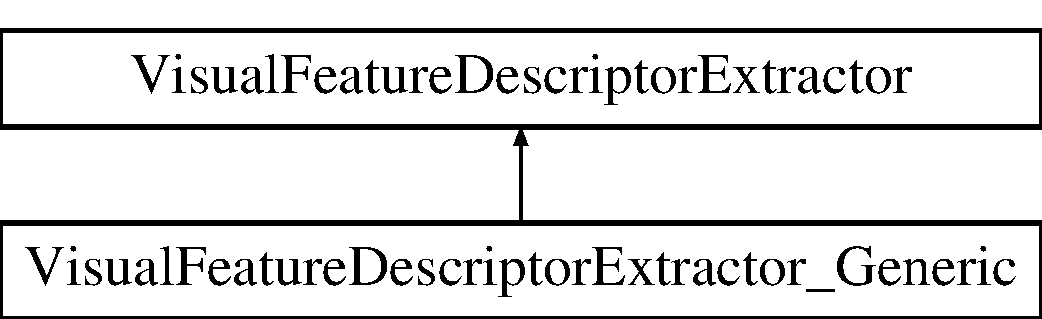
\includegraphics[height=2.000000cm]{class_visual_feature_descriptor_extractor___generic}
\end{center}
\end{figure}
\subsection*{Public Member Functions}
\begin{DoxyCompactItemize}
\item 
\hyperlink{class_visual_feature_descriptor_extractor___generic_ae3e5c7b0bc31689bb5d0eb408cd592b7}{VisualFeatureDescriptorExtractor\_\-Generic} (cv::Ptr$<$ cv::FeatureDetector $>$ featDetector, cv::Ptr$<$ cv::DescriptorExtractor $>$ descExtractor)
\item 
void \hyperlink{class_visual_feature_descriptor_extractor___generic_adec3d1c762c1010c2e95101822f688b7}{detectKeypointsAndComputeDescriptors} (std::vector$<$ cv::KeyPoint $>$ \&keypoints, cv::Mat \&descriptors, std::vector$<$ float $>$ \&descriptors\_\-aux)
\item 
void \hyperlink{class_visual_feature_descriptor_extractor___generic_a0027ad7b2b0196e31f1829c981488174}{detectKeypoints} (std::vector$<$ cv::KeyPoint $>$ \&keypoints)
\item 
void \hyperlink{class_visual_feature_descriptor_extractor___generic_ad878e967bcf2c00065fbc13af593ff46}{computeDescriptors} (std::vector$<$ cv::KeyPoint $>$ \&descriptors\_\-aux, cv::Mat \&descriptors)
\end{DoxyCompactItemize}
\subsection*{Private Attributes}
\begin{DoxyCompactItemize}
\item 
\hypertarget{class_visual_feature_descriptor_extractor___generic_a3bd14d4f99f9eea5a2b45432571aaac5}{
cv::Ptr$<$ cv::FeatureDetector $>$ {\bfseries featureDetector}}
\label{class_visual_feature_descriptor_extractor___generic_a3bd14d4f99f9eea5a2b45432571aaac5}

\item 
\hypertarget{class_visual_feature_descriptor_extractor___generic_aee24bd98238bee0e178f846c3c523c72}{
cv::Ptr$<$ cv::DescriptorExtractor $>$ {\bfseries descriptorExtractor}}
\label{class_visual_feature_descriptor_extractor___generic_aee24bd98238bee0e178f846c3c523c72}

\end{DoxyCompactItemize}


\subsection{Detailed Description}
This class encapsulates the functionality of a generic 2D visual feature detector and descriptor extractor using the OpenCV library. 

\subsection{Constructor \& Destructor Documentation}
\hypertarget{class_visual_feature_descriptor_extractor___generic_ae3e5c7b0bc31689bb5d0eb408cd592b7}{
\index{VisualFeatureDescriptorExtractor\_\-Generic@{VisualFeatureDescriptorExtractor\_\-Generic}!VisualFeatureDescriptorExtractor\_\-Generic@{VisualFeatureDescriptorExtractor\_\-Generic}}
\index{VisualFeatureDescriptorExtractor\_\-Generic@{VisualFeatureDescriptorExtractor\_\-Generic}!VisualFeatureDescriptorExtractor_Generic@{VisualFeatureDescriptorExtractor\_\-Generic}}
\subsubsection[{VisualFeatureDescriptorExtractor\_\-Generic}]{\setlength{\rightskip}{0pt plus 5cm}VisualFeatureDescriptorExtractor\_\-Generic::VisualFeatureDescriptorExtractor\_\-Generic (
\begin{DoxyParamCaption}
\item[{cv::Ptr$<$ cv::FeatureDetector $>$}]{featDetector, }
\item[{cv::Ptr$<$ cv::DescriptorExtractor $>$}]{descExtractor}
\end{DoxyParamCaption}
)}}
\label{class_visual_feature_descriptor_extractor___generic_ae3e5c7b0bc31689bb5d0eb408cd592b7}
Constructor of an instance of \hyperlink{class_visual_feature_descriptor_extractor___generic}{VisualFeatureDescriptorExtractor\_\-Generic} given a feature detector and descriptor extractor. 

\subsection{Member Function Documentation}
\hypertarget{class_visual_feature_descriptor_extractor___generic_ad878e967bcf2c00065fbc13af593ff46}{
\index{VisualFeatureDescriptorExtractor\_\-Generic@{VisualFeatureDescriptorExtractor\_\-Generic}!computeDescriptors@{computeDescriptors}}
\index{computeDescriptors@{computeDescriptors}!VisualFeatureDescriptorExtractor_Generic@{VisualFeatureDescriptorExtractor\_\-Generic}}
\subsubsection[{computeDescriptors}]{\setlength{\rightskip}{0pt plus 5cm}void VisualFeatureDescriptorExtractor\_\-Generic::computeDescriptors (
\begin{DoxyParamCaption}
\item[{std::vector$<$ cv::KeyPoint $>$ \&}]{descriptors\_\-aux, }
\item[{cv::Mat \&}]{descriptors}
\end{DoxyParamCaption}
)}}
\label{class_visual_feature_descriptor_extractor___generic_ad878e967bcf2c00065fbc13af593ff46}
Performs descriptor extraction over the image provided by the method setIntputImage. \hypertarget{class_visual_feature_descriptor_extractor___generic_a0027ad7b2b0196e31f1829c981488174}{
\index{VisualFeatureDescriptorExtractor\_\-Generic@{VisualFeatureDescriptorExtractor\_\-Generic}!detectKeypoints@{detectKeypoints}}
\index{detectKeypoints@{detectKeypoints}!VisualFeatureDescriptorExtractor_Generic@{VisualFeatureDescriptorExtractor\_\-Generic}}
\subsubsection[{detectKeypoints}]{\setlength{\rightskip}{0pt plus 5cm}void VisualFeatureDescriptorExtractor\_\-Generic::detectKeypoints (
\begin{DoxyParamCaption}
\item[{std::vector$<$ cv::KeyPoint $>$ \&}]{keypoints}
\end{DoxyParamCaption}
)}}
\label{class_visual_feature_descriptor_extractor___generic_a0027ad7b2b0196e31f1829c981488174}
Performs feature detection over the image provided by the method setInputImage. \hypertarget{class_visual_feature_descriptor_extractor___generic_adec3d1c762c1010c2e95101822f688b7}{
\index{VisualFeatureDescriptorExtractor\_\-Generic@{VisualFeatureDescriptorExtractor\_\-Generic}!detectKeypointsAndComputeDescriptors@{detectKeypointsAndComputeDescriptors}}
\index{detectKeypointsAndComputeDescriptors@{detectKeypointsAndComputeDescriptors}!VisualFeatureDescriptorExtractor_Generic@{VisualFeatureDescriptorExtractor\_\-Generic}}
\subsubsection[{detectKeypointsAndComputeDescriptors}]{\setlength{\rightskip}{0pt plus 5cm}void VisualFeatureDescriptorExtractor\_\-Generic::detectKeypointsAndComputeDescriptors (
\begin{DoxyParamCaption}
\item[{std::vector$<$ cv::KeyPoint $>$ \&}]{keypoints, }
\item[{cv::Mat \&}]{descriptors, }
\item[{std::vector$<$ float $>$ \&}]{descriptors\_\-aux}
\end{DoxyParamCaption}
)\hspace{0.3cm}{\ttfamily  \mbox{[}virtual\mbox{]}}}}
\label{class_visual_feature_descriptor_extractor___generic_adec3d1c762c1010c2e95101822f688b7}
Performs feature detection and descriptor extraction over the image provided by the method setInputImage. 

Implements \hyperlink{class_visual_feature_descriptor_extractor_aac4d313540ff83e03fb5b0a0952fc0f4}{VisualFeatureDescriptorExtractor}.



The documentation for this class was generated from the following file:\begin{DoxyCompactItemize}
\item 
VisualFeatureDescriptorExtractor\_\-Generic.h\end{DoxyCompactItemize}

\hypertarget{class_visual_feature_descriptor_extractor___o_r_b}{
\section{VisualFeatureDescriptorExtractor\_\-ORB Class Reference}
\label{class_visual_feature_descriptor_extractor___o_r_b}\index{VisualFeatureDescriptorExtractor\_\-ORB@{VisualFeatureDescriptorExtractor\_\-ORB}}
}


{\ttfamily \#include $<$VisualFeatureDescriptorExtractor\_\-ORB.h$>$}

Inheritance diagram for VisualFeatureDescriptorExtractor\_\-ORB:\begin{figure}[H]
\begin{center}
\leavevmode
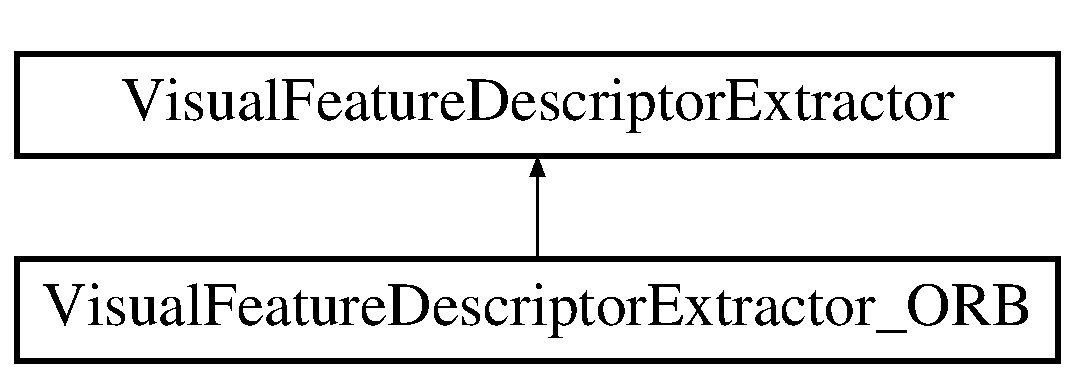
\includegraphics[height=2.000000cm]{class_visual_feature_descriptor_extractor___o_r_b}
\end{center}
\end{figure}
\subsection*{Public Member Functions}
\begin{DoxyCompactItemize}
\item 
void \hyperlink{class_visual_feature_descriptor_extractor___o_r_b_a2cded6e20e202bb6f2db3a64edeaffcf}{detectKeypointsAndComputeDescriptors} (std::vector$<$ cv::KeyPoint $>$ \&keypoints, cv::Mat \&descriptors, std::vector$<$ float $>$ \&descriptors\_\-aux)
\end{DoxyCompactItemize}
\subsection*{Private Attributes}
\begin{DoxyCompactItemize}
\item 
\hypertarget{class_visual_feature_descriptor_extractor___o_r_b_a07083d7edf26ab7fe0a12e270650517f}{
cv::ORB {\bfseries orb}}
\label{class_visual_feature_descriptor_extractor___o_r_b_a07083d7edf26ab7fe0a12e270650517f}

\end{DoxyCompactItemize}


\subsection{Detailed Description}
This class encapsulates the functionality of an ORB 2D visual feature detector and descriptor extractor using the OpenCV library. 

\subsection{Member Function Documentation}
\hypertarget{class_visual_feature_descriptor_extractor___o_r_b_a2cded6e20e202bb6f2db3a64edeaffcf}{
\index{VisualFeatureDescriptorExtractor\_\-ORB@{VisualFeatureDescriptorExtractor\_\-ORB}!detectKeypointsAndComputeDescriptors@{detectKeypointsAndComputeDescriptors}}
\index{detectKeypointsAndComputeDescriptors@{detectKeypointsAndComputeDescriptors}!VisualFeatureDescriptorExtractor_ORB@{VisualFeatureDescriptorExtractor\_\-ORB}}
\subsubsection[{detectKeypointsAndComputeDescriptors}]{\setlength{\rightskip}{0pt plus 5cm}void VisualFeatureDescriptorExtractor\_\-ORB::detectKeypointsAndComputeDescriptors (
\begin{DoxyParamCaption}
\item[{std::vector$<$ cv::KeyPoint $>$ \&}]{keypoints, }
\item[{cv::Mat \&}]{descriptors, }
\item[{std::vector$<$ float $>$ \&}]{descriptors\_\-aux}
\end{DoxyParamCaption}
)\hspace{0.3cm}{\ttfamily  \mbox{[}virtual\mbox{]}}}}
\label{class_visual_feature_descriptor_extractor___o_r_b_a2cded6e20e202bb6f2db3a64edeaffcf}
Performs ORB feature detection and descriptor extraction over the image provided by the method setInputImage. 

Implements \hyperlink{class_visual_feature_descriptor_extractor_aac4d313540ff83e03fb5b0a0952fc0f4}{VisualFeatureDescriptorExtractor}.



The documentation for this class was generated from the following file:\begin{DoxyCompactItemize}
\item 
VisualFeatureDescriptorExtractor\_\-ORB.h\end{DoxyCompactItemize}

\hypertarget{class_visual_feature_descriptor_extractor___s_u_r_f___g_p_u}{
\section{VisualFeatureDescriptorExtractor\_\-SURF\_\-GPU Class Reference}
\label{class_visual_feature_descriptor_extractor___s_u_r_f___g_p_u}\index{VisualFeatureDescriptorExtractor\_\-SURF\_\-GPU@{VisualFeatureDescriptorExtractor\_\-SURF\_\-GPU}}
}


{\ttfamily \#include $<$VisualFeatureDescriptorExtractor\_\-SURF\_\-GPU.h$>$}

Inheritance diagram for VisualFeatureDescriptorExtractor\_\-SURF\_\-GPU:\begin{figure}[H]
\begin{center}
\leavevmode
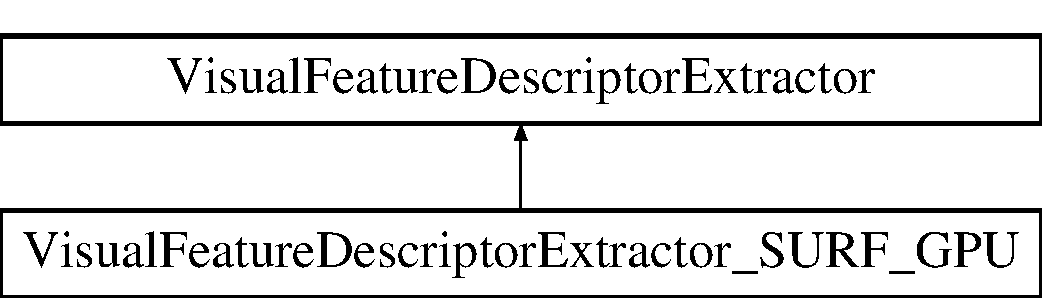
\includegraphics[height=2.000000cm]{class_visual_feature_descriptor_extractor___s_u_r_f___g_p_u}
\end{center}
\end{figure}
\subsection*{Public Member Functions}
\begin{DoxyCompactItemize}
\item 
void \hyperlink{class_visual_feature_descriptor_extractor___s_u_r_f___g_p_u_aef7ddf1d1e42267ba7b5d06a0a36e58f}{detectKeypointsAndComputeDescriptors} (std::vector$<$ cv::KeyPoint $>$ \&keypoints, cv::Mat \&descriptors, std::vector$<$ float $>$ \&descriptors\_\-aux)
\end{DoxyCompactItemize}
\subsection*{Private Attributes}
\begin{DoxyCompactItemize}
\item 
\hypertarget{class_visual_feature_descriptor_extractor___s_u_r_f___g_p_u_a6c5740d8a8de3d2010a02c524bf54bd7}{
cv::gpu::SURF\_\-GPU {\bfseries surf}}
\label{class_visual_feature_descriptor_extractor___s_u_r_f___g_p_u_a6c5740d8a8de3d2010a02c524bf54bd7}

\item 
\hypertarget{class_visual_feature_descriptor_extractor___s_u_r_f___g_p_u_a5fbe8308ae8cb7c0e2743dcbd7ac9291}{
std::vector$<$ float $>$ {\bfseries descriptors\_\-aux}}
\label{class_visual_feature_descriptor_extractor___s_u_r_f___g_p_u_a5fbe8308ae8cb7c0e2743dcbd7ac9291}

\item 
\hypertarget{class_visual_feature_descriptor_extractor___s_u_r_f___g_p_u_ab18da50bfdc5aa8a233937fcfe5eedc1}{
cv::gpu::GpuMat {\bfseries imgMatGPU}}
\label{class_visual_feature_descriptor_extractor___s_u_r_f___g_p_u_ab18da50bfdc5aa8a233937fcfe5eedc1}

\item 
\hypertarget{class_visual_feature_descriptor_extractor___s_u_r_f___g_p_u_a550538d586f31def7935183111acb19b}{
cv::gpu::GpuMat {\bfseries keypointsGPU}}
\label{class_visual_feature_descriptor_extractor___s_u_r_f___g_p_u_a550538d586f31def7935183111acb19b}

\item 
\hypertarget{class_visual_feature_descriptor_extractor___s_u_r_f___g_p_u_a2410bf2aa3e2330e4ae7d141ff8179d6}{
cv::gpu::GpuMat {\bfseries descriptorsGPU}}
\label{class_visual_feature_descriptor_extractor___s_u_r_f___g_p_u_a2410bf2aa3e2330e4ae7d141ff8179d6}

\end{DoxyCompactItemize}


\subsection{Detailed Description}
This class encapsulates the functionality of a SURF 2D visual feature detector and descriptor extractor using the OpenCV library and CUDA. This class integrates a GPU accelerated implementation of SURF. 

\subsection{Member Function Documentation}
\hypertarget{class_visual_feature_descriptor_extractor___s_u_r_f___g_p_u_aef7ddf1d1e42267ba7b5d06a0a36e58f}{
\index{VisualFeatureDescriptorExtractor\_\-SURF\_\-GPU@{VisualFeatureDescriptorExtractor\_\-SURF\_\-GPU}!detectKeypointsAndComputeDescriptors@{detectKeypointsAndComputeDescriptors}}
\index{detectKeypointsAndComputeDescriptors@{detectKeypointsAndComputeDescriptors}!VisualFeatureDescriptorExtractor_SURF_GPU@{VisualFeatureDescriptorExtractor\_\-SURF\_\-GPU}}
\subsubsection[{detectKeypointsAndComputeDescriptors}]{\setlength{\rightskip}{0pt plus 5cm}void VisualFeatureDescriptorExtractor\_\-SURF\_\-GPU::detectKeypointsAndComputeDescriptors (
\begin{DoxyParamCaption}
\item[{std::vector$<$ cv::KeyPoint $>$ \&}]{keypoints, }
\item[{cv::Mat \&}]{descriptors, }
\item[{std::vector$<$ float $>$ \&}]{descriptors\_\-aux}
\end{DoxyParamCaption}
)\hspace{0.3cm}{\ttfamily  \mbox{[}virtual\mbox{]}}}}
\label{class_visual_feature_descriptor_extractor___s_u_r_f___g_p_u_aef7ddf1d1e42267ba7b5d06a0a36e58f}
Performs SURF feature detection and descriptor extraction over the image provided by the method setInputImage. 

Implements \hyperlink{class_visual_feature_descriptor_extractor_aac4d313540ff83e03fb5b0a0952fc0f4}{VisualFeatureDescriptorExtractor}.



The documentation for this class was generated from the following file:\begin{DoxyCompactItemize}
\item 
VisualFeatureDescriptorExtractor\_\-SURF\_\-GPU.h\end{DoxyCompactItemize}

\hypertarget{class_visual_feature_matcher}{
\section{VisualFeatureMatcher Class Reference}
\label{class_visual_feature_matcher}\index{VisualFeatureMatcher@{VisualFeatureMatcher}}
}


{\ttfamily \#include $<$VisualFeatureMatcher.h$>$}

Inheritance diagram for VisualFeatureMatcher:\begin{figure}[H]
\begin{center}
\leavevmode
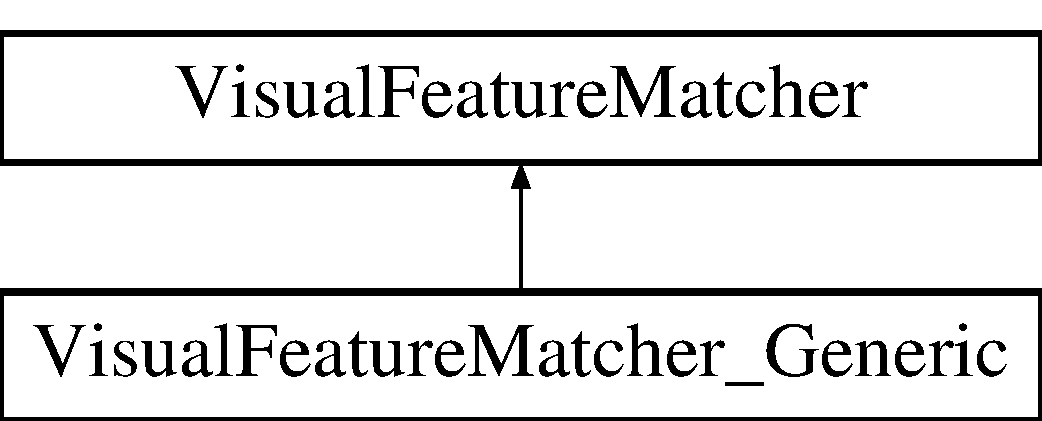
\includegraphics[height=2.000000cm]{class_visual_feature_matcher}
\end{center}
\end{figure}
\subsection*{Public Member Functions}
\begin{DoxyCompactItemize}
\item 
virtual void \hyperlink{class_visual_feature_matcher_a4e70d34d256b19bf4a1dbc1ee14c0e91}{match} (const cv::Mat \&descriptors1, const cv::Mat \&descriptors2, std::vector$<$ cv::DMatch $>$ \&matches)=0
\end{DoxyCompactItemize}


\subsection{Detailed Description}
Abstract class that specifies a method to perform 2D visual feature matching. 

\subsection{Member Function Documentation}
\hypertarget{class_visual_feature_matcher_a4e70d34d256b19bf4a1dbc1ee14c0e91}{
\index{VisualFeatureMatcher@{VisualFeatureMatcher}!match@{match}}
\index{match@{match}!VisualFeatureMatcher@{VisualFeatureMatcher}}
\subsubsection[{match}]{\setlength{\rightskip}{0pt plus 5cm}virtual void VisualFeatureMatcher::match (
\begin{DoxyParamCaption}
\item[{const cv::Mat \&}]{descriptors1, }
\item[{const cv::Mat \&}]{descriptors2, }
\item[{std::vector$<$ cv::DMatch $>$ \&}]{matches}
\end{DoxyParamCaption}
)\hspace{0.3cm}{\ttfamily  \mbox{[}pure virtual\mbox{]}}}}
\label{class_visual_feature_matcher_a4e70d34d256b19bf4a1dbc1ee14c0e91}
Performs descriptors matching and returns a vector of 2D matches. For every descriptor in descriptors1, the method computes the nearest descriptor in descriptors2. 

Implemented in \hyperlink{class_visual_feature_matcher___generic_a8c45652a033f333938f5440486cd6fa9}{VisualFeatureMatcher\_\-Generic}.



The documentation for this class was generated from the following file:\begin{DoxyCompactItemize}
\item 
VisualFeatureMatcher.h\end{DoxyCompactItemize}

\hypertarget{class_visual_feature_matcher___generic}{
\section{VisualFeatureMatcher\_\-Generic Class Reference}
\label{class_visual_feature_matcher___generic}\index{VisualFeatureMatcher\_\-Generic@{VisualFeatureMatcher\_\-Generic}}
}


{\ttfamily \#include $<$VisualFeatureMatcher\_\-Generic.h$>$}

Inheritance diagram for VisualFeatureMatcher\_\-Generic:\begin{figure}[H]
\begin{center}
\leavevmode
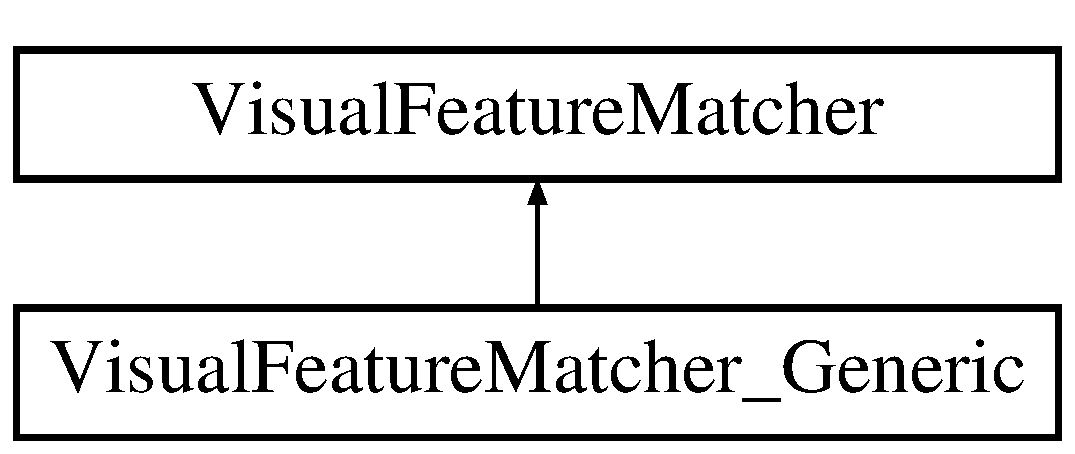
\includegraphics[height=2.000000cm]{class_visual_feature_matcher___generic}
\end{center}
\end{figure}
\subsection*{Public Member Functions}
\begin{DoxyCompactItemize}
\item 
\hyperlink{class_visual_feature_matcher___generic_afb3206845d3f219b2da647b4224e5785}{VisualFeatureMatcher\_\-Generic} (cv::Ptr$<$ cv::DescriptorMatcher $>$ matcher, const std::string \&matchingAlgorithm)
\item 
void \hyperlink{class_visual_feature_matcher___generic_a4dd886147652cc05b8ae1b77f41c50dd}{crossCheckMatching} (const cv::Mat \&descriptors1, const cv::Mat \&descriptors2, std::vector$<$ cv::DMatch $>$ \&matches)
\item 
void \hyperlink{class_visual_feature_matcher___generic_a78cfb12bdfc7c9c3e8e1191630713a4f}{simpleMatching} (const cv::Mat \&descriptors1, const cv::Mat \&descriptors2, std::vector$<$ cv::DMatch $>$ \&matches)
\item 
void \hyperlink{class_visual_feature_matcher___generic_a8c45652a033f333938f5440486cd6fa9}{match} (const cv::Mat \&descriptors1, const cv::Mat \&descriptors2, std::vector$<$ cv::DMatch $>$ \&matches)
\item 
int \hyperlink{class_visual_feature_matcher___generic_a6f1654953bbd83f954bdbe1ed711fced}{outlierRemovalHomography} (const std::vector$<$ cv::KeyPoint $>$ \&keypoints1, const std::vector$<$ cv::KeyPoint $>$ \&keypoints2, const std::vector$<$ cv::DMatch $>$ \&matches, std::vector$<$ char $>$ \&matchesMask, const double ransacInlierDistance=3.0)
\item 
int \hyperlink{class_visual_feature_matcher___generic_a5fe8fbffca8ad33423eea2af12d34273}{outlierRemovalFundamentalMat} (const std::vector$<$ cv::KeyPoint $>$ \&keypoints1, const std::vector$<$ cv::KeyPoint $>$ \&keypoints2, const std::vector$<$ cv::DMatch $>$ \&matches, std::vector$<$ char $>$ \&matchesMask, const double ransacInlierDistance=3.0)
\item 
void \hyperlink{class_visual_feature_matcher___generic_a0adf4907dc8492986a013e2f7ba0931d}{get2DMatchedPoints} (const std::vector$<$ cv::KeyPoint $>$ \&keypoints1, const std::vector$<$ cv::KeyPoint $>$ \&keypoints2, const std::vector$<$ cv::DMatch $>$ \&matches, std::vector$<$ cv::Point2f $>$ \&points1, std::vector$<$ cv::Point2f $>$ \&points2, const int numberInliers, const std::vector$<$ char $>$ \&matchesMask)
\item 
void \hyperlink{class_visual_feature_matcher___generic_af473e2359dece0aaf1a5a31c357cfaac}{get2DMatchedPoints} (const std::vector$<$ cv::KeyPoint $>$ \&keypoints1, const std::vector$<$ cv::KeyPoint $>$ \&keypoints2, const std::vector$<$ cv::DMatch $>$ \&matches, std::vector$<$ cv::Point2f $>$ \&points1, std::vector$<$ cv::Point2f $>$ \&points2)
\end{DoxyCompactItemize}
\subsection*{Protected Types}
\begin{DoxyCompactItemize}
\item 
enum \{ {\bfseries NONE\_\-FILTER} =  0, 
{\bfseries CROSS\_\-CHECK\_\-FILTER} =  1
 \}
\end{DoxyCompactItemize}
\subsection*{Protected Attributes}
\begin{DoxyCompactItemize}
\item 
\hypertarget{class_visual_feature_matcher___generic_af342f1e9d8e90dfcb7ad3f3fea7133cf}{
cv::Ptr$<$ cv::DescriptorMatcher $>$ {\bfseries descriptorMatcher}}
\label{class_visual_feature_matcher___generic_af342f1e9d8e90dfcb7ad3f3fea7133cf}

\item 
\hypertarget{class_visual_feature_matcher___generic_a00f0156439c360533af21f05226f4fd4}{
int {\bfseries matcherFilterType}}
\label{class_visual_feature_matcher___generic_a00f0156439c360533af21f05226f4fd4}

\end{DoxyCompactItemize}


\subsection{Detailed Description}
This class encapsulates the functionality of a generic 2D feature descriptor matcher using the OpenCV library. 

\subsection{Constructor \& Destructor Documentation}
\hypertarget{class_visual_feature_matcher___generic_afb3206845d3f219b2da647b4224e5785}{
\index{VisualFeatureMatcher\_\-Generic@{VisualFeatureMatcher\_\-Generic}!VisualFeatureMatcher\_\-Generic@{VisualFeatureMatcher\_\-Generic}}
\index{VisualFeatureMatcher\_\-Generic@{VisualFeatureMatcher\_\-Generic}!VisualFeatureMatcher_Generic@{VisualFeatureMatcher\_\-Generic}}
\subsubsection[{VisualFeatureMatcher\_\-Generic}]{\setlength{\rightskip}{0pt plus 5cm}VisualFeatureMatcher\_\-Generic::VisualFeatureMatcher\_\-Generic (
\begin{DoxyParamCaption}
\item[{cv::Ptr$<$ cv::DescriptorMatcher $>$}]{matcher, }
\item[{const std::string \&}]{matchingAlgorithm}
\end{DoxyParamCaption}
)}}
\label{class_visual_feature_matcher___generic_afb3206845d3f219b2da647b4224e5785}
Creates an instance of \hyperlink{class_visual_feature_matcher___generic}{VisualFeatureMatcher\_\-Generic} given a descriptor matcher a std::string that specifies the matching algorithm.
\begin{DoxyItemize}
\item \char`\"{}NoneFilter\char`\"{}: Computes the nearest descriptors of descriptors1 in descriptors2 and returns the vector of matches.
\item \char`\"{}CrossCheckFilter\char`\"{}: Computes the nearest descriptors of descriptors1 in descriptors2 (forward matching). Then it computes the nearest descriptors of descriptors2 in descriptors1 (backward matching). It then retains the matches that appears in both forward and backward matching. 
\end{DoxyItemize}

\subsection{Member Function Documentation}
\hypertarget{class_visual_feature_matcher___generic_a4dd886147652cc05b8ae1b77f41c50dd}{
\index{VisualFeatureMatcher\_\-Generic@{VisualFeatureMatcher\_\-Generic}!crossCheckMatching@{crossCheckMatching}}
\index{crossCheckMatching@{crossCheckMatching}!VisualFeatureMatcher_Generic@{VisualFeatureMatcher\_\-Generic}}
\subsubsection[{crossCheckMatching}]{\setlength{\rightskip}{0pt plus 5cm}void VisualFeatureMatcher\_\-Generic::crossCheckMatching (
\begin{DoxyParamCaption}
\item[{const cv::Mat \&}]{descriptors1, }
\item[{const cv::Mat \&}]{descriptors2, }
\item[{std::vector$<$ cv::DMatch $>$ \&}]{matches}
\end{DoxyParamCaption}
)}}
\label{class_visual_feature_matcher___generic_a4dd886147652cc05b8ae1b77f41c50dd}
Performs descriptor matching using the Cross Check Filter algorithm. Computes the nearest descriptors of descriptors1 in descriptors2 (forward matching). Then it computes the nearest descriptors of descriptors2 in descriptors1 (backward matching). It then retains the matches that appears in both forward and backward matching. \hypertarget{class_visual_feature_matcher___generic_af473e2359dece0aaf1a5a31c357cfaac}{
\index{VisualFeatureMatcher\_\-Generic@{VisualFeatureMatcher\_\-Generic}!get2DMatchedPoints@{get2DMatchedPoints}}
\index{get2DMatchedPoints@{get2DMatchedPoints}!VisualFeatureMatcher_Generic@{VisualFeatureMatcher\_\-Generic}}
\subsubsection[{get2DMatchedPoints}]{\setlength{\rightskip}{0pt plus 5cm}void VisualFeatureMatcher\_\-Generic::get2DMatchedPoints (
\begin{DoxyParamCaption}
\item[{const std::vector$<$ cv::KeyPoint $>$ \&}]{keypoints1, }
\item[{const std::vector$<$ cv::KeyPoint $>$ \&}]{keypoints2, }
\item[{const std::vector$<$ cv::DMatch $>$ \&}]{matches, }
\item[{std::vector$<$ cv::Point2f $>$ \&}]{points1, }
\item[{std::vector$<$ cv::Point2f $>$ \&}]{points2}
\end{DoxyParamCaption}
)}}
\label{class_visual_feature_matcher___generic_af473e2359dece0aaf1a5a31c357cfaac}
This method takes the keypoints and matches to obtain two vectors of 2D points with the pairs of 2D correspondences of each match. \hypertarget{class_visual_feature_matcher___generic_a0adf4907dc8492986a013e2f7ba0931d}{
\index{VisualFeatureMatcher\_\-Generic@{VisualFeatureMatcher\_\-Generic}!get2DMatchedPoints@{get2DMatchedPoints}}
\index{get2DMatchedPoints@{get2DMatchedPoints}!VisualFeatureMatcher_Generic@{VisualFeatureMatcher\_\-Generic}}
\subsubsection[{get2DMatchedPoints}]{\setlength{\rightskip}{0pt plus 5cm}void VisualFeatureMatcher\_\-Generic::get2DMatchedPoints (
\begin{DoxyParamCaption}
\item[{const std::vector$<$ cv::KeyPoint $>$ \&}]{keypoints1, }
\item[{const std::vector$<$ cv::KeyPoint $>$ \&}]{keypoints2, }
\item[{const std::vector$<$ cv::DMatch $>$ \&}]{matches, }
\item[{std::vector$<$ cv::Point2f $>$ \&}]{points1, }
\item[{std::vector$<$ cv::Point2f $>$ \&}]{points2, }
\item[{const int}]{numberInliers, }
\item[{const std::vector$<$ char $>$ \&}]{matchesMask}
\end{DoxyParamCaption}
)}}
\label{class_visual_feature_matcher___generic_a0adf4907dc8492986a013e2f7ba0931d}
This method takes the keypoints, matches and matchesMask to obtain two vectors of 2D points with the pairs of 2D correspondences of each match. \hypertarget{class_visual_feature_matcher___generic_a8c45652a033f333938f5440486cd6fa9}{
\index{VisualFeatureMatcher\_\-Generic@{VisualFeatureMatcher\_\-Generic}!match@{match}}
\index{match@{match}!VisualFeatureMatcher_Generic@{VisualFeatureMatcher\_\-Generic}}
\subsubsection[{match}]{\setlength{\rightskip}{0pt plus 5cm}void VisualFeatureMatcher\_\-Generic::match (
\begin{DoxyParamCaption}
\item[{const cv::Mat \&}]{descriptors1, }
\item[{const cv::Mat \&}]{descriptors2, }
\item[{std::vector$<$ cv::DMatch $>$ \&}]{matches}
\end{DoxyParamCaption}
)\hspace{0.3cm}{\ttfamily  \mbox{[}virtual\mbox{]}}}}
\label{class_visual_feature_matcher___generic_a8c45652a033f333938f5440486cd6fa9}
Performs descriptor matching. Computes simpleMatching or crossCheckMatching depending on the name of the algorithm specified when creating the instance of \hyperlink{class_visual_feature_matcher___generic}{VisualFeatureMatcher\_\-Generic}. 

Implements \hyperlink{class_visual_feature_matcher_a4e70d34d256b19bf4a1dbc1ee14c0e91}{VisualFeatureMatcher}.

\hypertarget{class_visual_feature_matcher___generic_a5fe8fbffca8ad33423eea2af12d34273}{
\index{VisualFeatureMatcher\_\-Generic@{VisualFeatureMatcher\_\-Generic}!outlierRemovalFundamentalMat@{outlierRemovalFundamentalMat}}
\index{outlierRemovalFundamentalMat@{outlierRemovalFundamentalMat}!VisualFeatureMatcher_Generic@{VisualFeatureMatcher\_\-Generic}}
\subsubsection[{outlierRemovalFundamentalMat}]{\setlength{\rightskip}{0pt plus 5cm}int VisualFeatureMatcher\_\-Generic::outlierRemovalFundamentalMat (
\begin{DoxyParamCaption}
\item[{const std::vector$<$ cv::KeyPoint $>$ \&}]{keypoints1, }
\item[{const std::vector$<$ cv::KeyPoint $>$ \&}]{keypoints2, }
\item[{const std::vector$<$ cv::DMatch $>$ \&}]{matches, }
\item[{std::vector$<$ char $>$ \&}]{matchesMask, }
\item[{const double}]{ransacInlierDistance = {\ttfamily 3.0}}
\end{DoxyParamCaption}
)}}
\label{class_visual_feature_matcher___generic_a5fe8fbffca8ad33423eea2af12d34273}
Performs outlier rejection with the fundamental matrix. This method computes the fundamental matrix that best fits the 2D matches using RANSAC and then rejects the 2D correspondences that doesn't fit the model to get robust 2D correspondences. This method returns the resulting number of inliers. \hypertarget{class_visual_feature_matcher___generic_a6f1654953bbd83f954bdbe1ed711fced}{
\index{VisualFeatureMatcher\_\-Generic@{VisualFeatureMatcher\_\-Generic}!outlierRemovalHomography@{outlierRemovalHomography}}
\index{outlierRemovalHomography@{outlierRemovalHomography}!VisualFeatureMatcher_Generic@{VisualFeatureMatcher\_\-Generic}}
\subsubsection[{outlierRemovalHomography}]{\setlength{\rightskip}{0pt plus 5cm}int VisualFeatureMatcher\_\-Generic::outlierRemovalHomography (
\begin{DoxyParamCaption}
\item[{const std::vector$<$ cv::KeyPoint $>$ \&}]{keypoints1, }
\item[{const std::vector$<$ cv::KeyPoint $>$ \&}]{keypoints2, }
\item[{const std::vector$<$ cv::DMatch $>$ \&}]{matches, }
\item[{std::vector$<$ char $>$ \&}]{matchesMask, }
\item[{const double}]{ransacInlierDistance = {\ttfamily 3.0}}
\end{DoxyParamCaption}
)}}
\label{class_visual_feature_matcher___generic_a6f1654953bbd83f954bdbe1ed711fced}
Performs outlier rejection with the homography matrix. This method computes the homography matrix that best fits the 2D matches using RANSAC and then rejects the 2D correspondences that doesn't fit the model to get robust 2D correspondences. This method returns the resulting number of inliers. \hypertarget{class_visual_feature_matcher___generic_a78cfb12bdfc7c9c3e8e1191630713a4f}{
\index{VisualFeatureMatcher\_\-Generic@{VisualFeatureMatcher\_\-Generic}!simpleMatching@{simpleMatching}}
\index{simpleMatching@{simpleMatching}!VisualFeatureMatcher_Generic@{VisualFeatureMatcher\_\-Generic}}
\subsubsection[{simpleMatching}]{\setlength{\rightskip}{0pt plus 5cm}void VisualFeatureMatcher\_\-Generic::simpleMatching (
\begin{DoxyParamCaption}
\item[{const cv::Mat \&}]{descriptors1, }
\item[{const cv::Mat \&}]{descriptors2, }
\item[{std::vector$<$ cv::DMatch $>$ \&}]{matches}
\end{DoxyParamCaption}
)}}
\label{class_visual_feature_matcher___generic_a78cfb12bdfc7c9c3e8e1191630713a4f}
Performs descriptor matching. Computes the nearest descriptors of descriptors1 in descriptors2 and returns a vector of matches. 

The documentation for this class was generated from the following file:\begin{DoxyCompactItemize}
\item 
VisualFeatureMatcher\_\-Generic.h\end{DoxyCompactItemize}

\printindex
\end{document}
